\section{Menù principale}
\subsection{Main activity}
Una volta effettuata la registrazione o login l'applicazione mostra la schermata principale.
\begin{figure}[H] 
	\centering 
	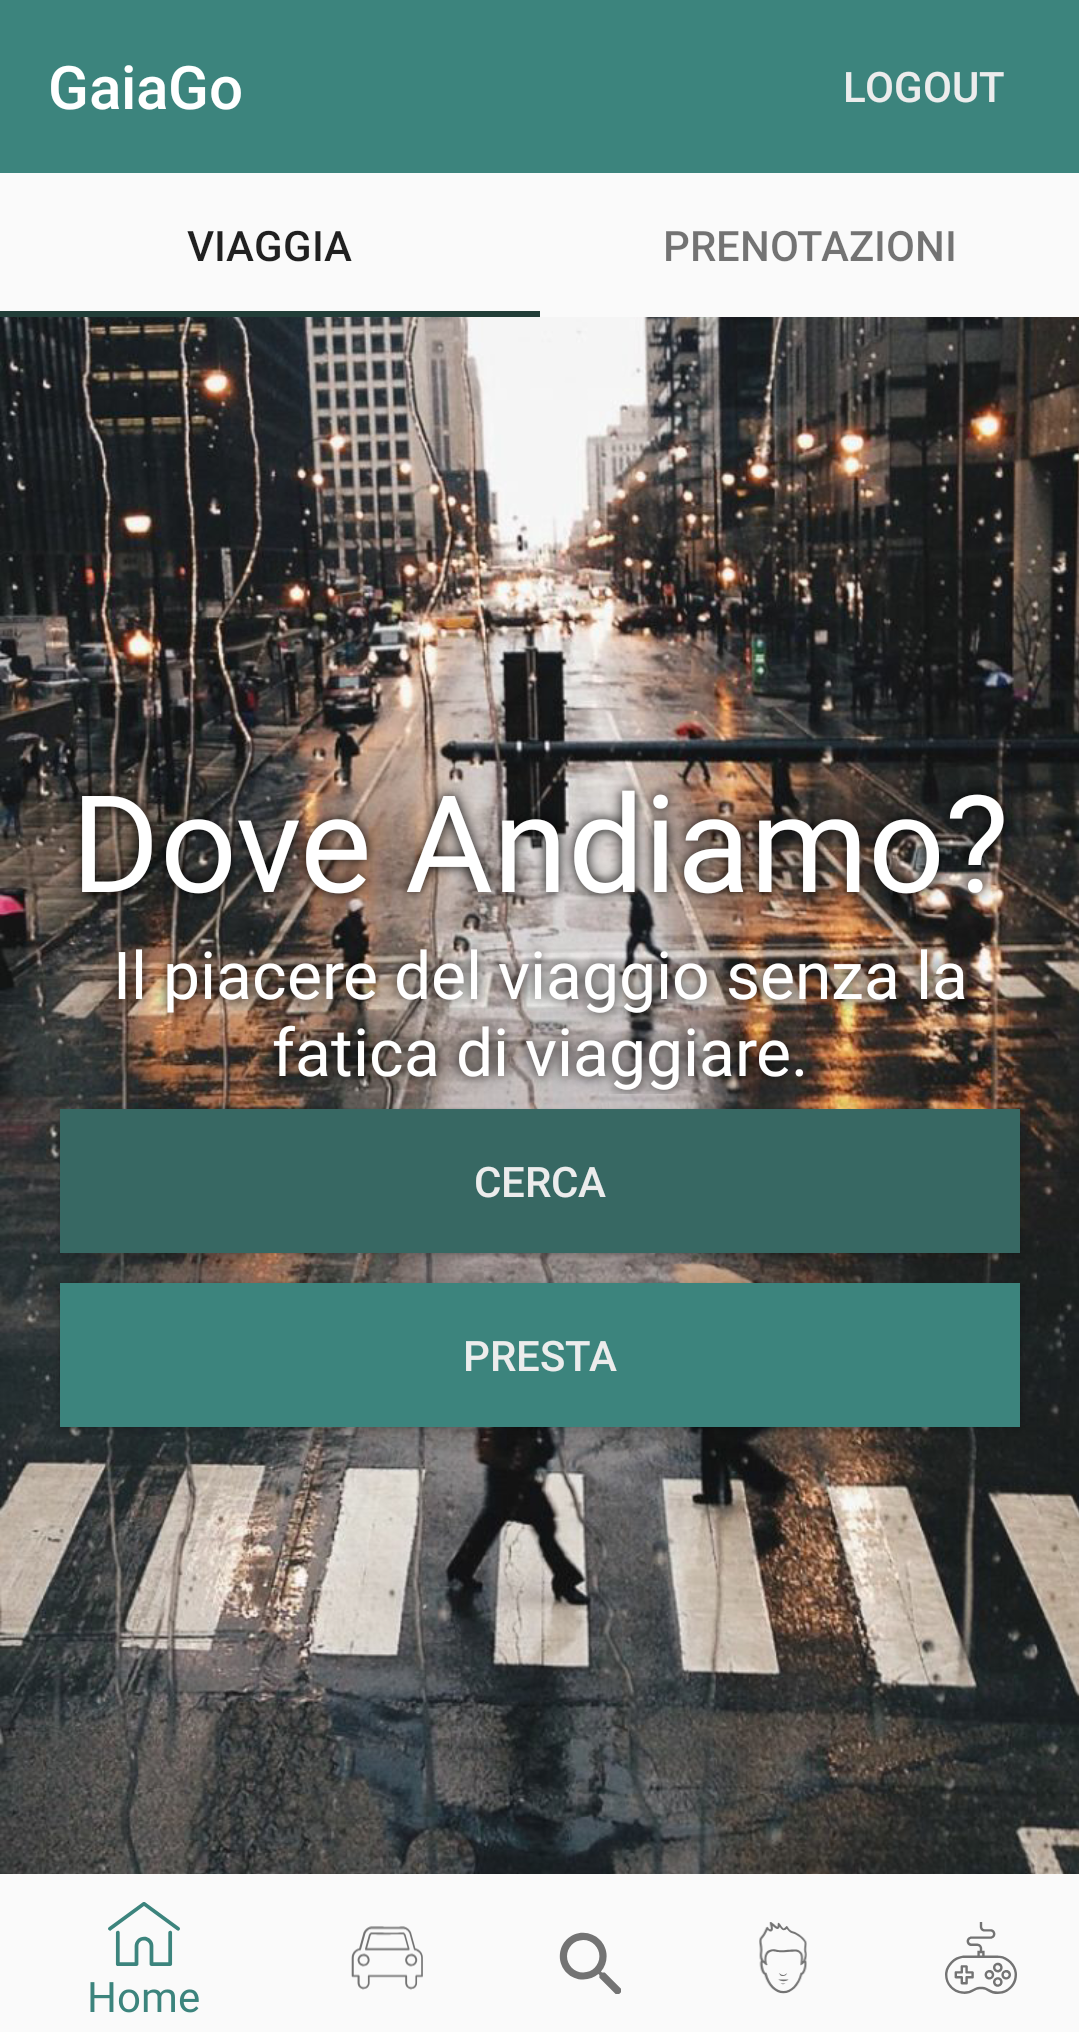
\includegraphics[width=0.5\textwidth]{res/images/home.png}\\
	\caption{Main activity}
	\label{Login}
\end{figure}
\pagebreak 
Da questa sezione è possibile accedere alle seguenti funzionalità:
\begin{itemize}
	\item \textbf{Viaggia}: in questa sezione sono presenti due pulsanti "CERCA" che riporta all'attività descritta nella sezione \ref{ricerca0} e il pulsante "PRESTA" che riporta, invece, alla sezione \ref{veicolo} dove viene descritta la relativa funzione;
	\item \textbf{Prenotazioni}: questa sezione comprende le funzionalità di gestione della prenotazione di un veicolo che viene descritta nel dettaglio nella sezione \ref{gestione}.
\end{itemize}
\begin{figure}[H] 
	\centering 
	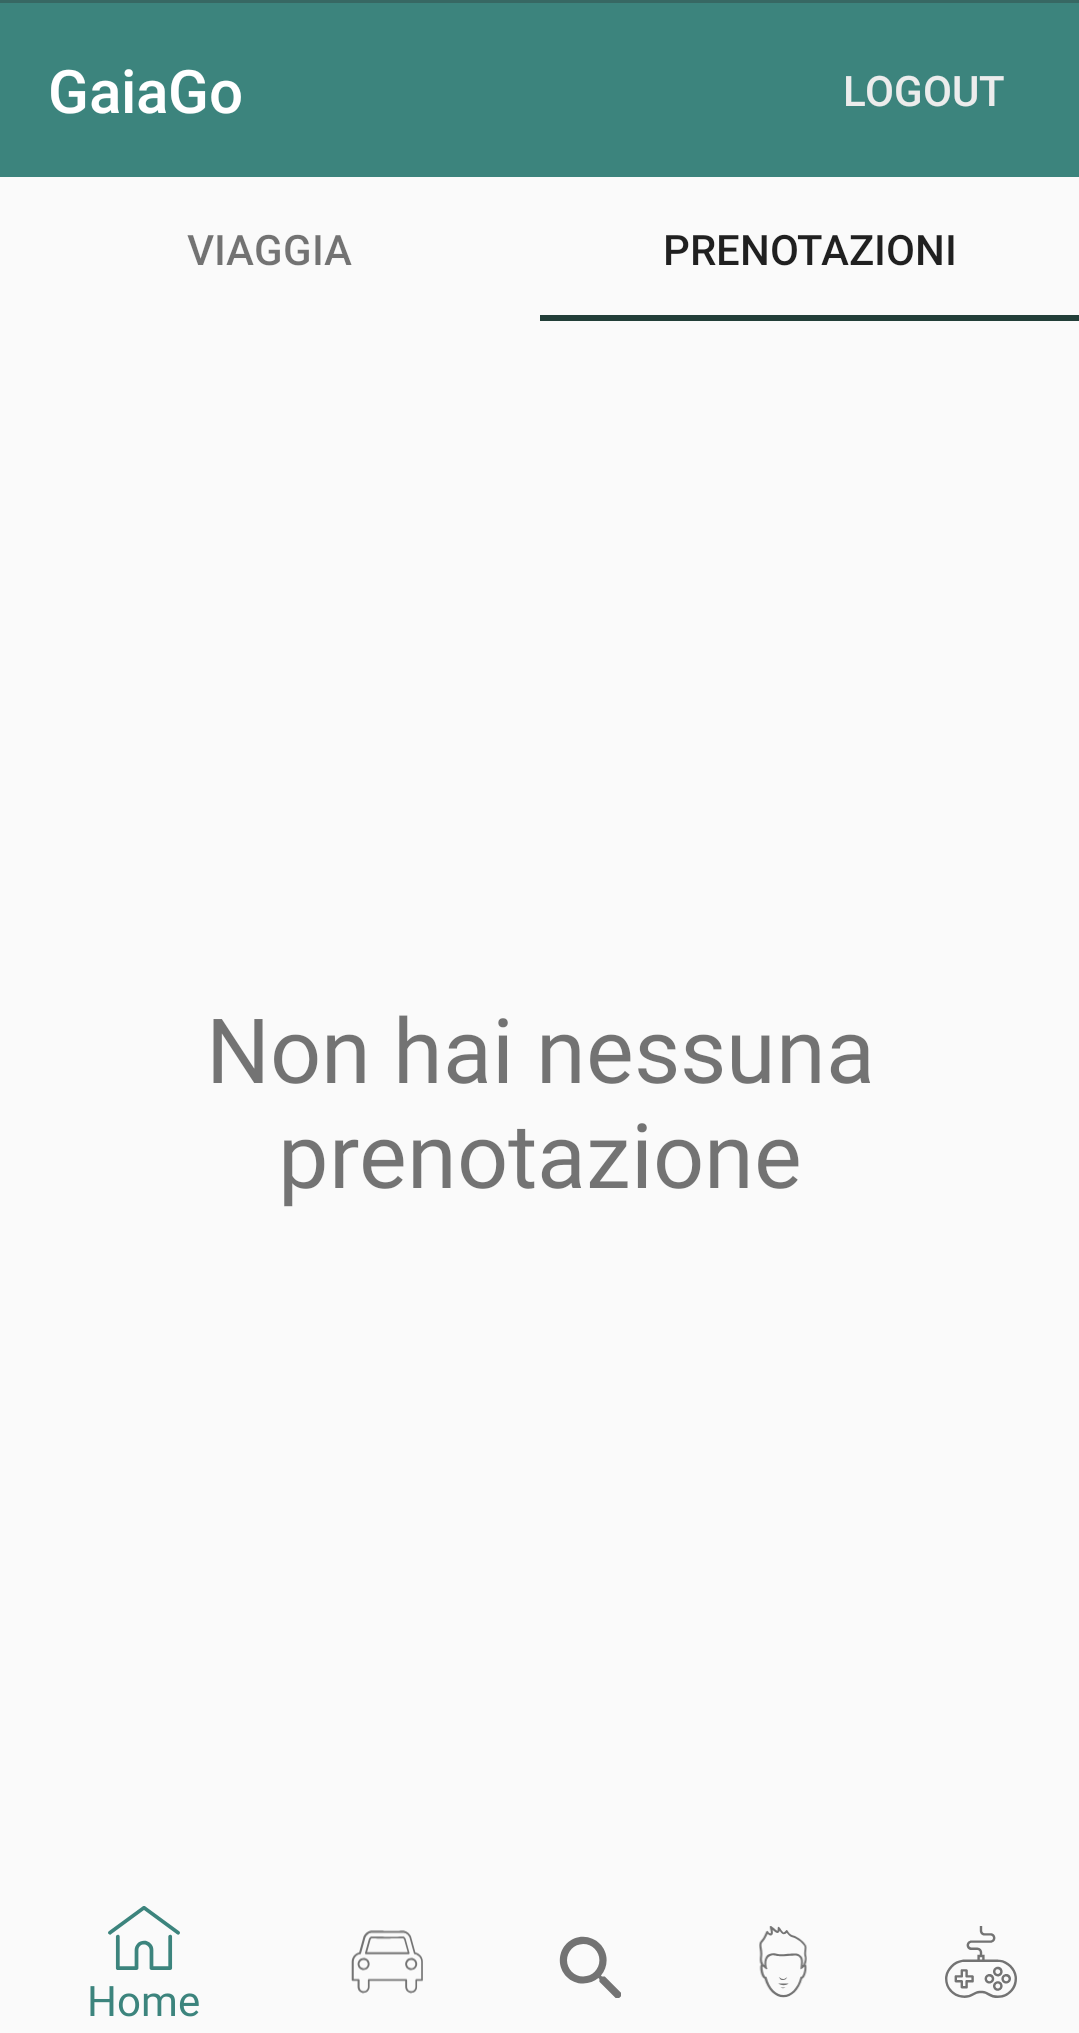
\includegraphics[width=0.5\textwidth]{res/images/prenotazioni.png}\\
	\caption{Main activity}
	\label{Login1}
\end{figure}
\pagebreak
\subsection{Logout e barra di navigazione}
Andiamo ora ad analizzare due parti fondamentali presenti in tutte e cinque le activity\glosp principali:
\begin{itemize}
	\item \textbf{Logout}: presente in alto a destra, permette all'utente di scollegare l'account in uso da \textit{Gaiago} e riporta alla schermata di login;
	\\\\
	  \begin{figure}[H] 
	 	\centering 
	 	
\includegraphics[width=0.5\textwidth]{res/images/logout.png}\\
	 	\caption{Bottone di logout}
	 	\label{Login button}
	 \end{figure}
 Una volta premuto compare il seguente dialog\glosp per chiedere la conferma.
 \\\\
 \begin{figure}[H] 
 	\centering 
 	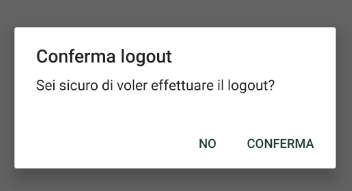
\includegraphics[width=0.5\textwidth]{res/images/logout_press.png}\\
 	\caption{Dialog logout}
 	\label{Logout_press}
 \end{figure}
 	\item  \textbf{Barra di navigazione}: presente in basso, permette all'utente di muoversi tra le varie funzionalità principali di \textit{GaiaGo}.
 	\\\\
 	  \begin{figure}[H] 
 	  	\centering 
 	  	
\includegraphics[width=0.5\textwidth]{res/images/barra_navigazione.png}\\
 	  	\caption{Barra di navigazione}
 	  	\label{Barra di navigazione}
 	  \end{figure}
\end{itemize}
\pagebreak
\subsection{Gestione veicoli}
\label{veicolo}
La gestione dei veicoli si trova nell'attività principale, più precisamente nella barra di navigazione dove è rappresentata da un automobile stilizzata e con la scritta "Auto" se ci si trova al suo interno.
 \begin{figure}[H] 
	\centering 
	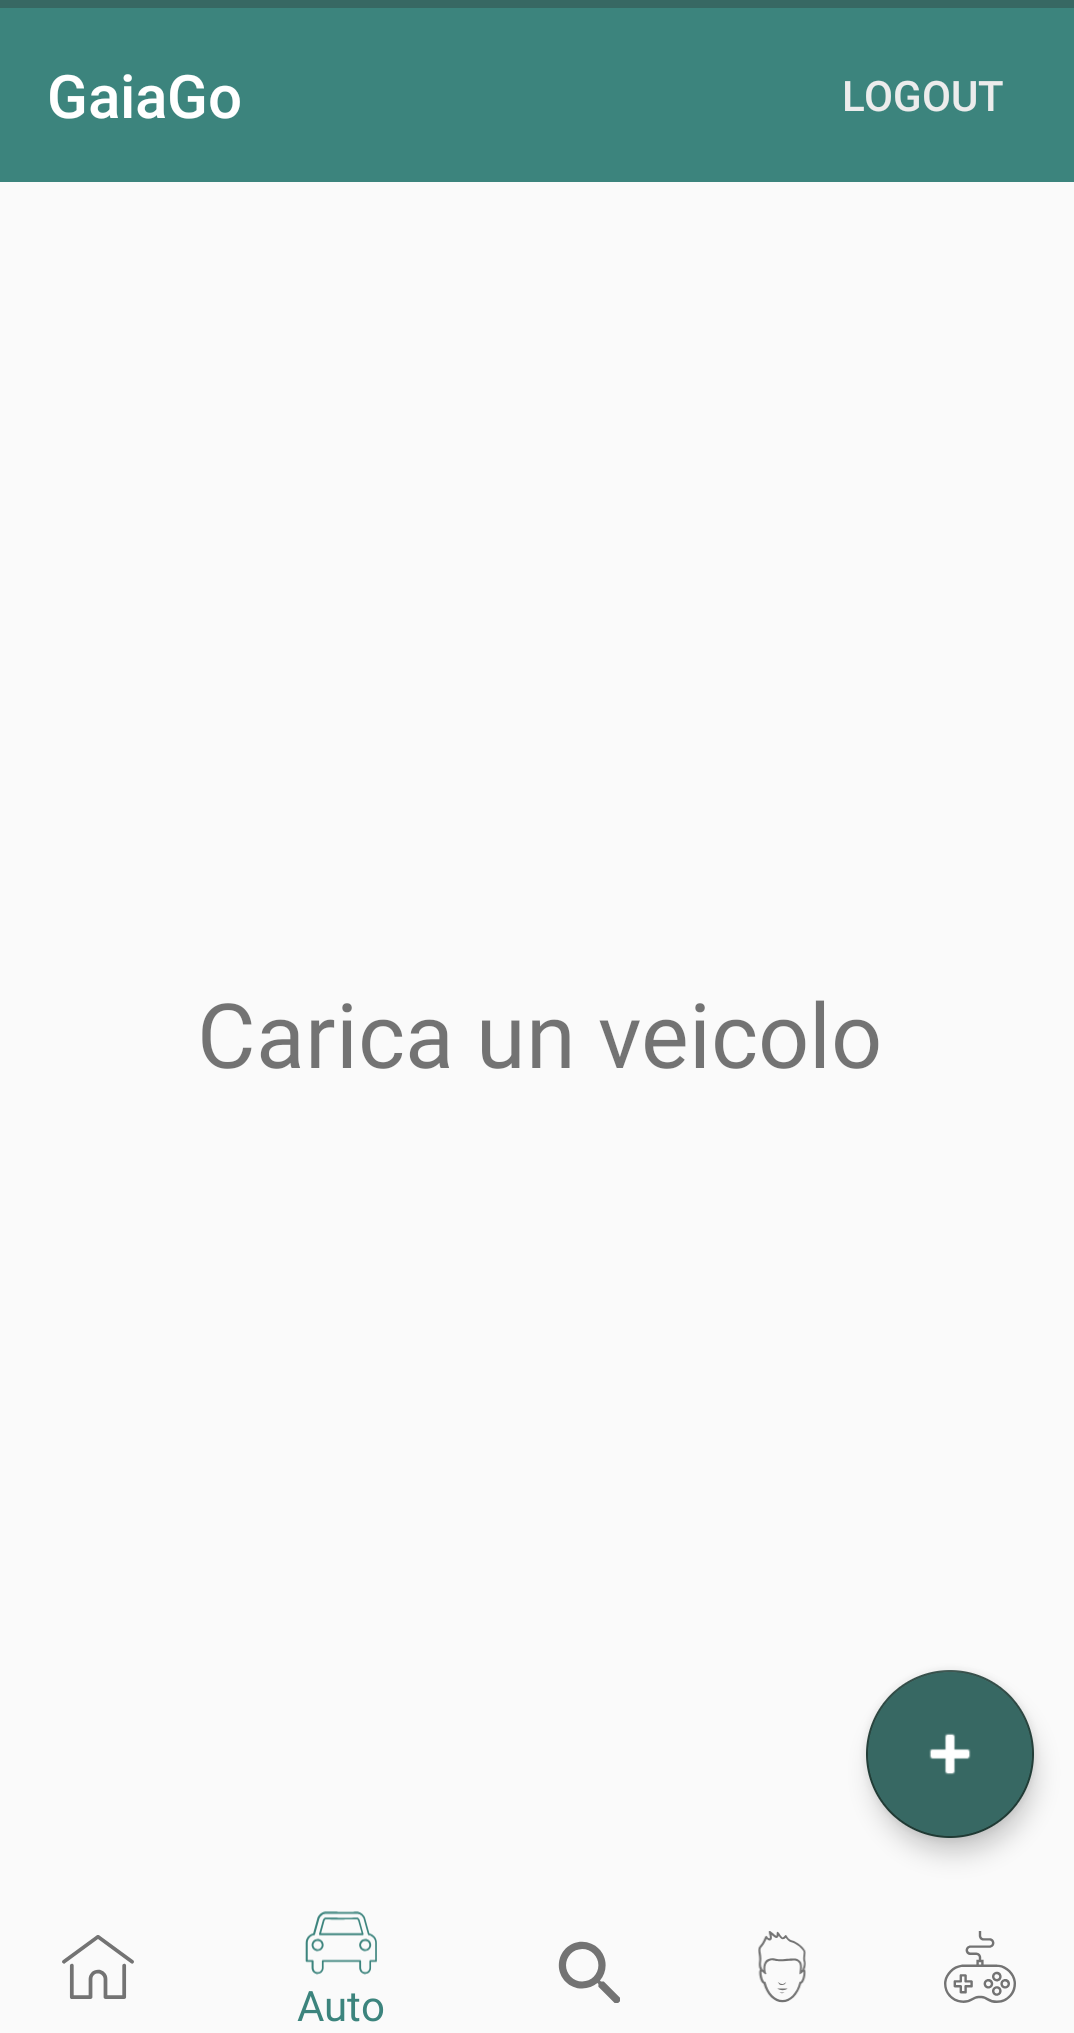
\includegraphics[width=0.5\textwidth]{res/images/gestione_veicolo.png}\\
	\caption{Gestione veicoli}
	\label{main}
\end{figure}
\pagebreak
\subsubsection{Inserimento veicolo}
All'utente è consentito di caricare i propri veicoli all'interno di \textit{GaiaGo}, per fare ciò, dalla schermata in cui sono presenti i propri veicoli (o non ve ne sono perché ancora da caricare), si preme il bottone verde contrassegnato da una "+" bianca.
Si viene portati ad una attività secondaria la quale permette l'inserimento dei dati del veicolo seguenti:
\begin{itemize}
	\item \textbf{foto}: è necessario inserire una foto del proprio veicolo per renderlo riconoscibile agli altri utenti, per fare ciò si preme il bottone verde contrassegnato da una "+" bianca.
	 \begin{figure}[H] 
		\centering 
		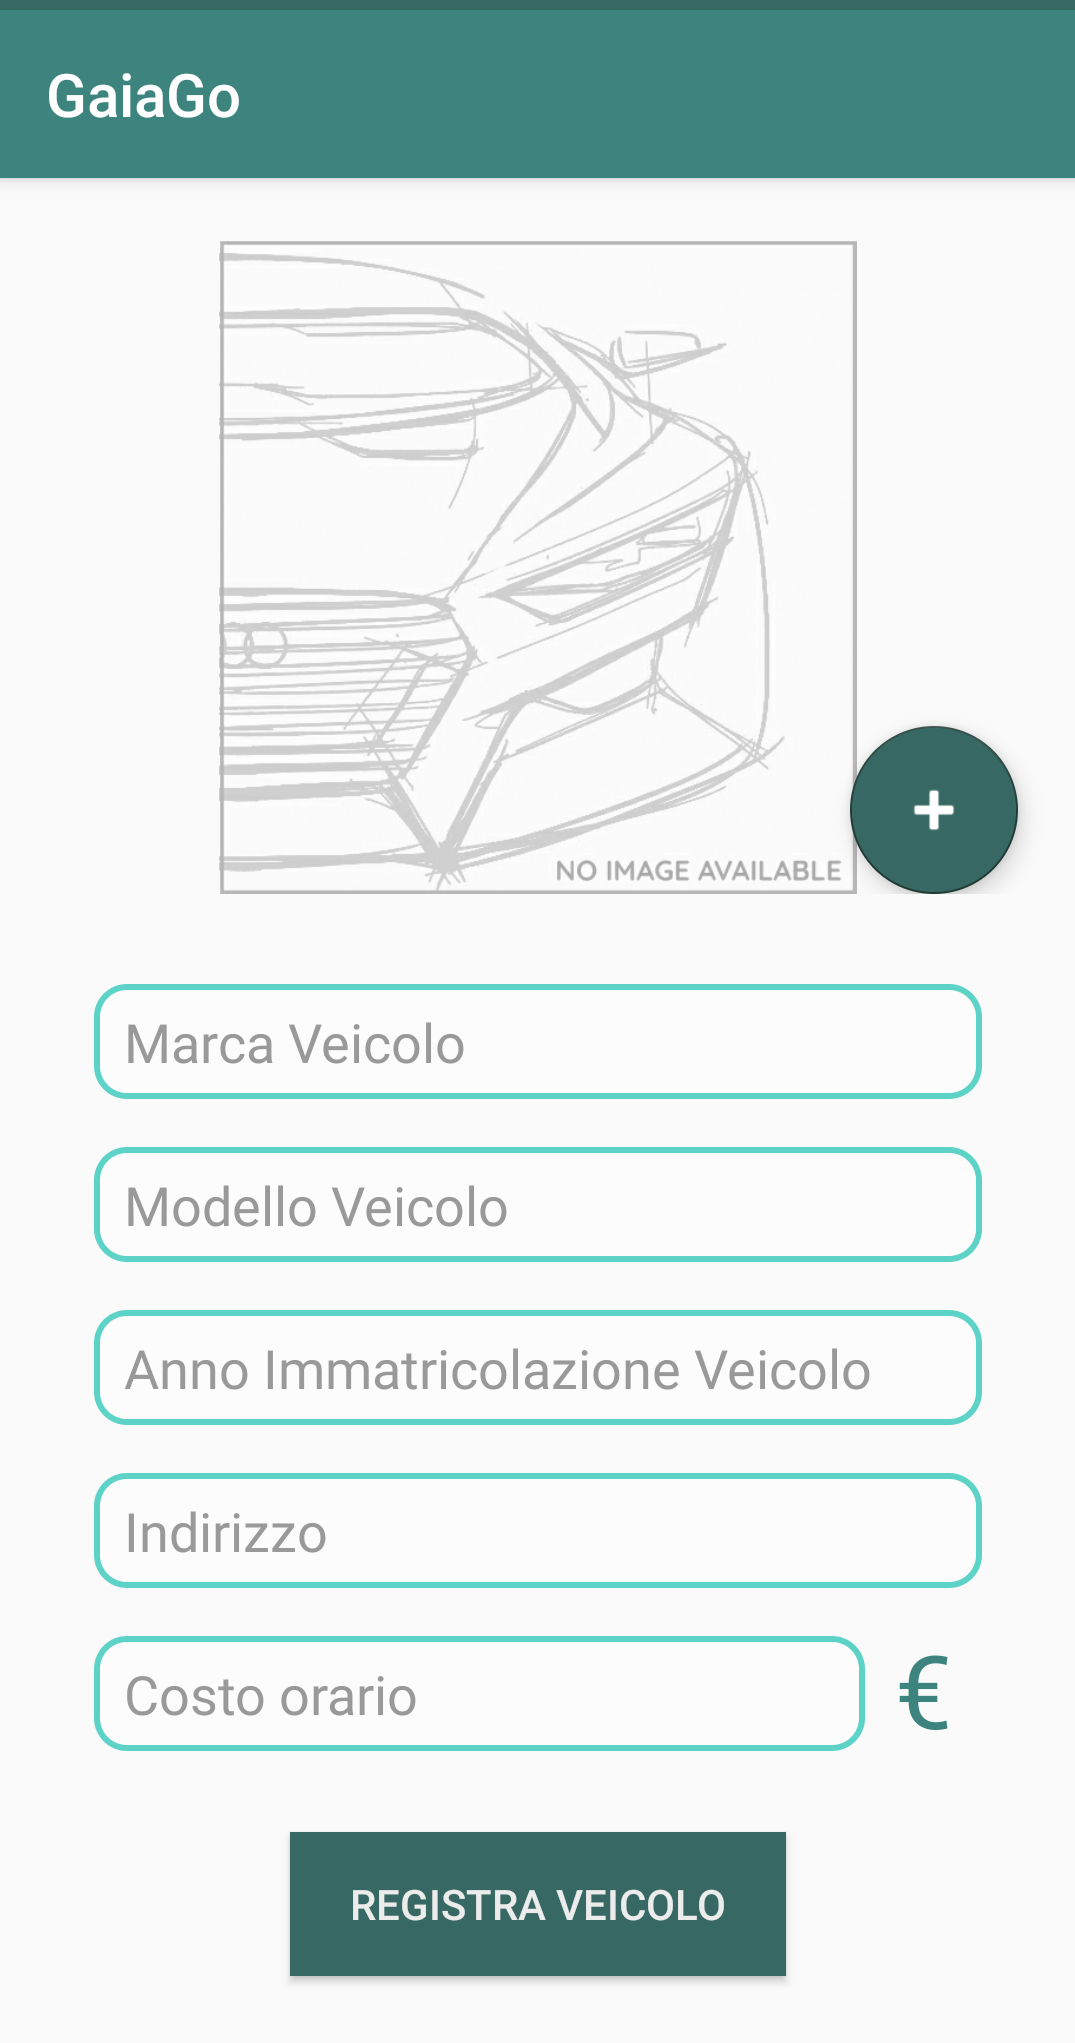
\includegraphics[width=0.5\textwidth]{res/images/caricamento_veicolo.png}\\
		\caption{Inserimento veicolo}
		\label{ins}
	\end{figure}
\pagebreak
Una volta premuto il pulsante si deve scegliere da dove caricare l'immagine e successivamente si preme sull'immagine da inserire;
 \begin{figure}[H] 
	\centering 
	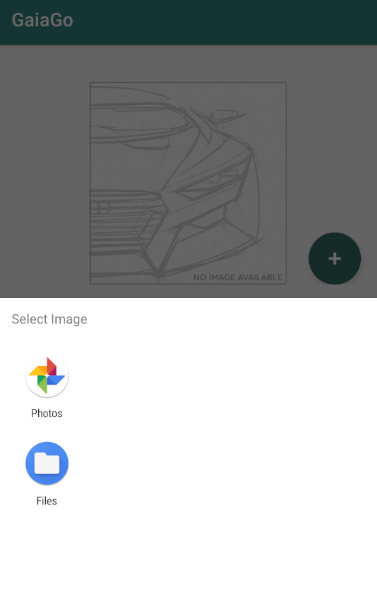
\includegraphics[width=0.5\textwidth]{res/images/caricamento_veicolo_bottone_premuto.png}\\
	\caption{Scelta immagine}
	\label{img}
\end{figure}
\pagebreak
\item \textbf{marca}: in questa sezione si sceglie la marca del proprio veicolo, per velocizzare ciò è reso disponibile un algoritmo di ricerca dinamico per l'auto-completamento;
 \begin{figure}[H] 
	\centering 
	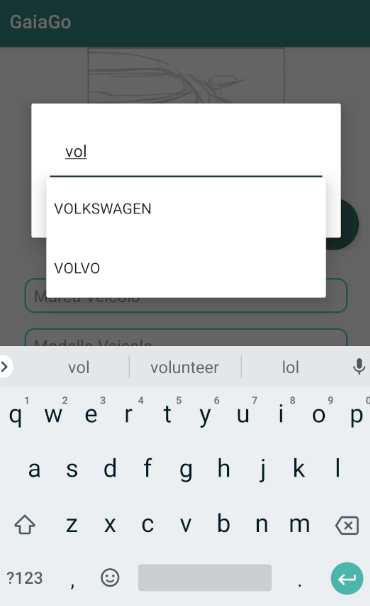
\includegraphics[width=0.5\textwidth]{res/images/marca_auto.png}\\
	\caption{Scelta marca}
	\label{marca}
\end{figure}
\pagebreak
\item \textbf{modello}: in questa sezione si sceglie il modello del proprio veicolo, per velocizzare ciò è reso disponibile un algoritmo di ricerca dinamico per l'auto-completamento;
 \begin{figure}[H] 
	\centering 
	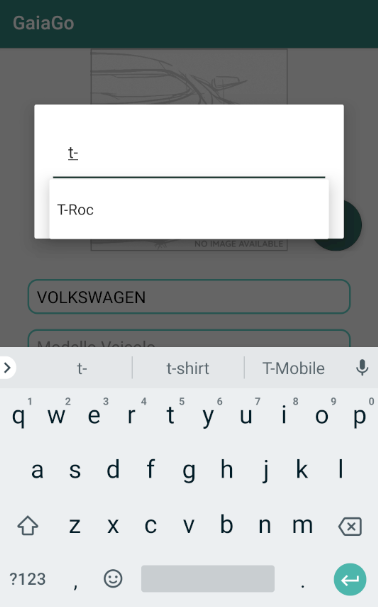
\includegraphics[width=0.5\textwidth]{res/images/modello_auto.png}\\
	\caption{Scelta modello}
	\label{modello}
\end{figure}
\item \textbf{anno d'immatricolazione}: in questa sezione si sceglie l'anno d'immatricolazione del proprio veicolo tramite un semplice editor di testo che non viene riportato in figura;
\pagebreak
\item \textbf{Indirizzo}: in questa sezione si inserisce l'indirizzo dove si trova il proprio veicolo, l'indirizzo è geo-localizzato grazie all'uso di un tool\glosp offerto da \textit{Google} il quale ci permette in seguito di ricercare i veicoli in base alla loro posizione sulla mappa. Anche qui è presente l'auto-completamento quindi possono essere inseriti solo indirizzi validi altrimenti non sarà possibile localizzare la reale posizione del veicolo;
 \begin{figure}[H] 
	\centering 
	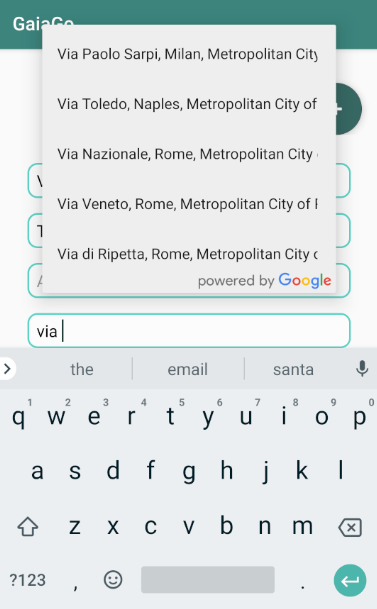
\includegraphics[width=0.5\textwidth]{res/images/indirizzo_auto.png}\\
	\caption{Scelta indirizzo}
	\label{indirizzo}
\end{figure}
\item \textbf{Costo orario}: in questa sezione si inserisce il costo orario fisso che si vuole mettere al veicolo avendo solamente la possibilità di inserire solo numeri. 
\end{itemize}
Per completare l'inserimento è necessario aver compilato tutti i campi richiesti quindi si preme il bottone verde "REGISTRA VEICOLO".
\pagebreak

\subsection{Inserimento disponibilità}
Nella schermata principale di visualizzazione dei veicoli è possibile, premendo su uno di essi, vedere i dettagli di quest'ultimo e si ha la possibilità di rimuoverlo dall'applicazione, visualizzarne le statistiche oppure di visualizzare le disponibilità aggiunte al veicolo. Una volta presenti nella schermata del veicolo si preme sul pulsante "VISUALIZZA DISPONIBILITà".
\begin{figure}[H] 
	\centering 
	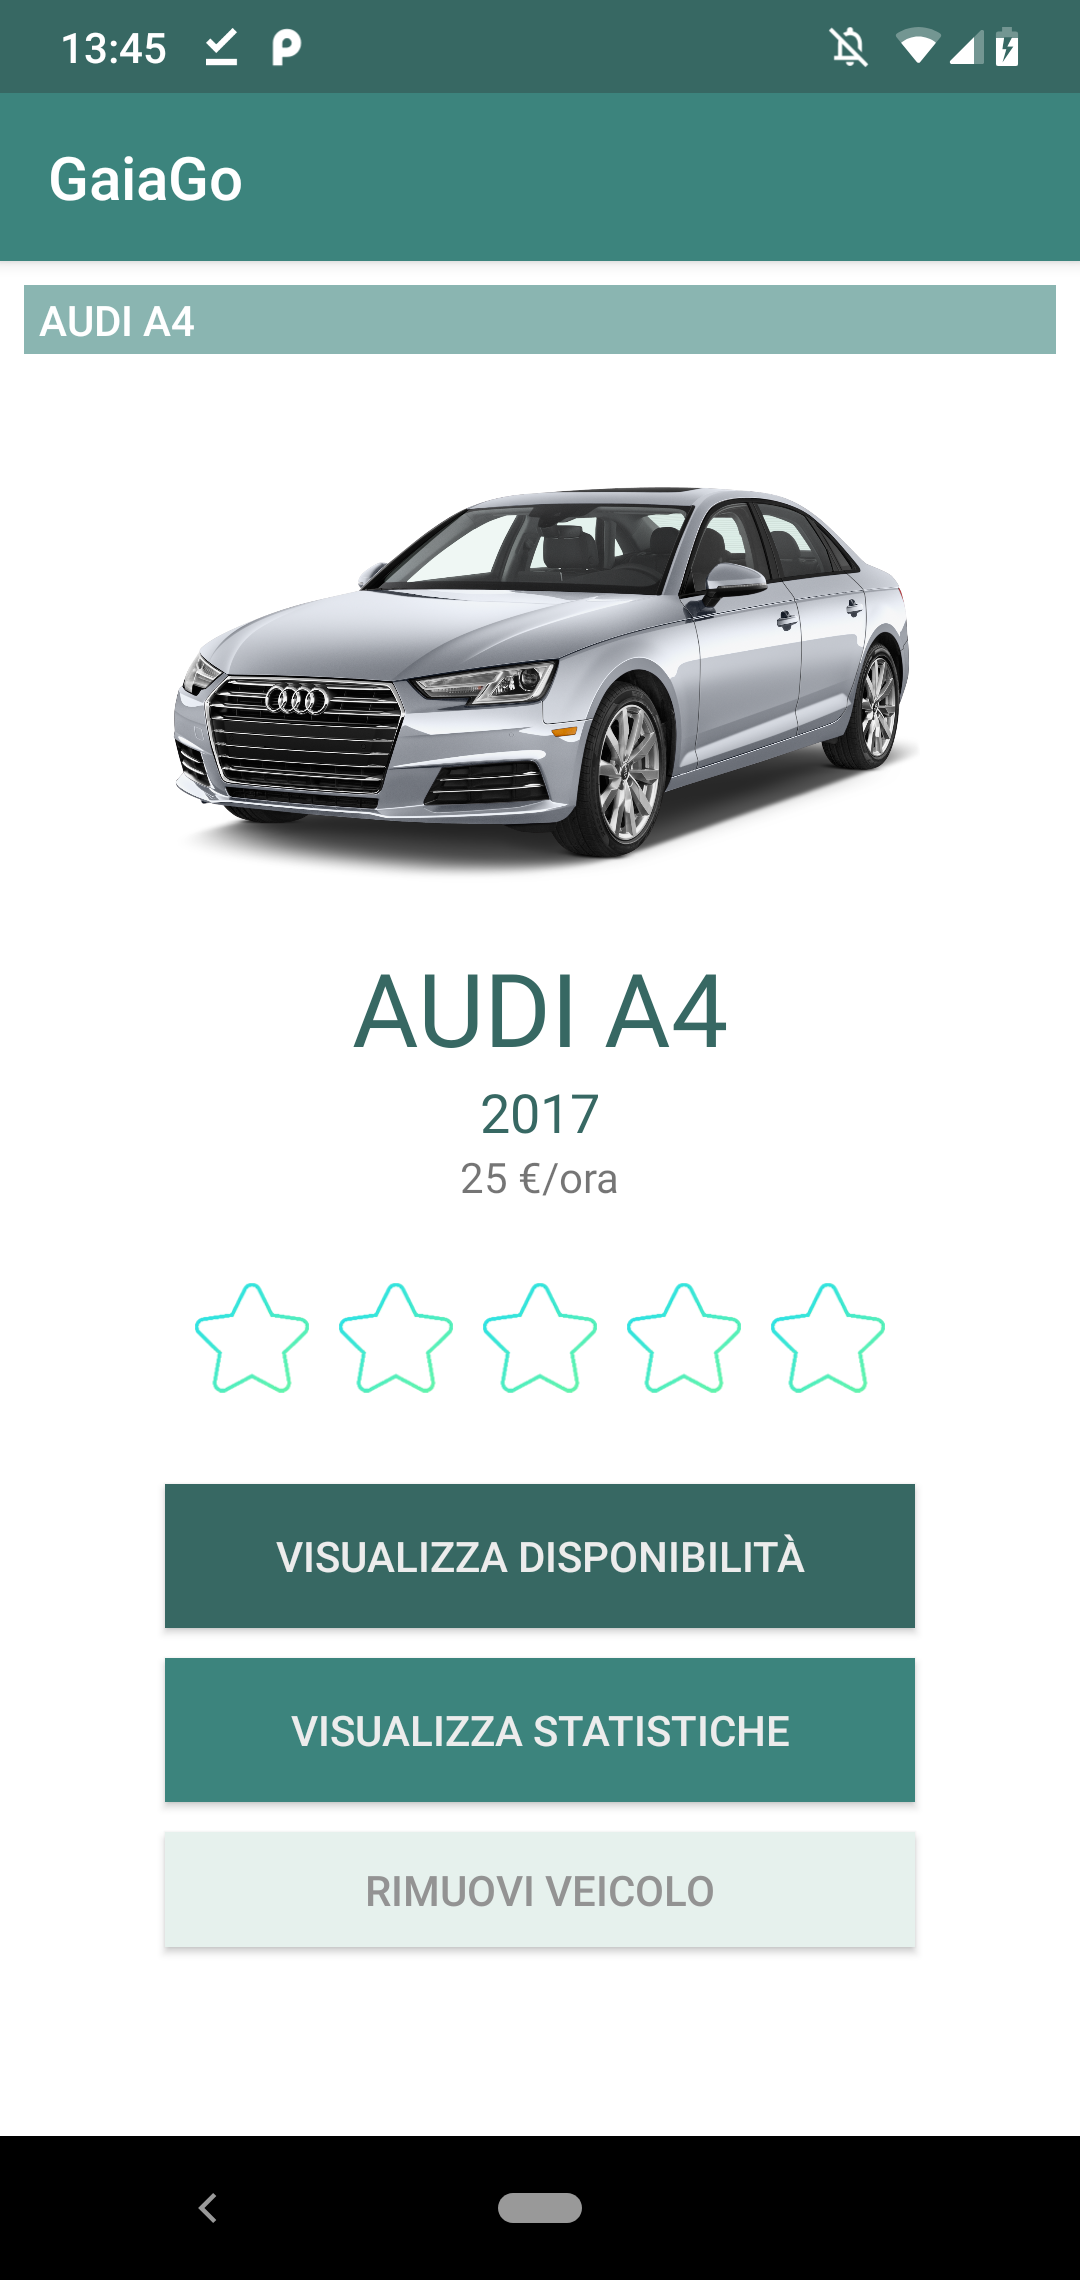
\includegraphics[width=0.5\textwidth]{res/images/visualizza_dettagli.png}\\
	\caption{Visualizza dettagli veicolo}
	\label{disponibilità}
\end{figure}
\pagebreak
Una volta premuto il pulsante si passa alla visualizzazione delle disponibilità fino ad ora inserite dall'utente proprietario del veicolo. A questo punto l'utente attraverso il pulsante "+" potrà aggiungere ulteriori disponibilità al veicolo.
\begin{figure}[H] 
	\centering 
	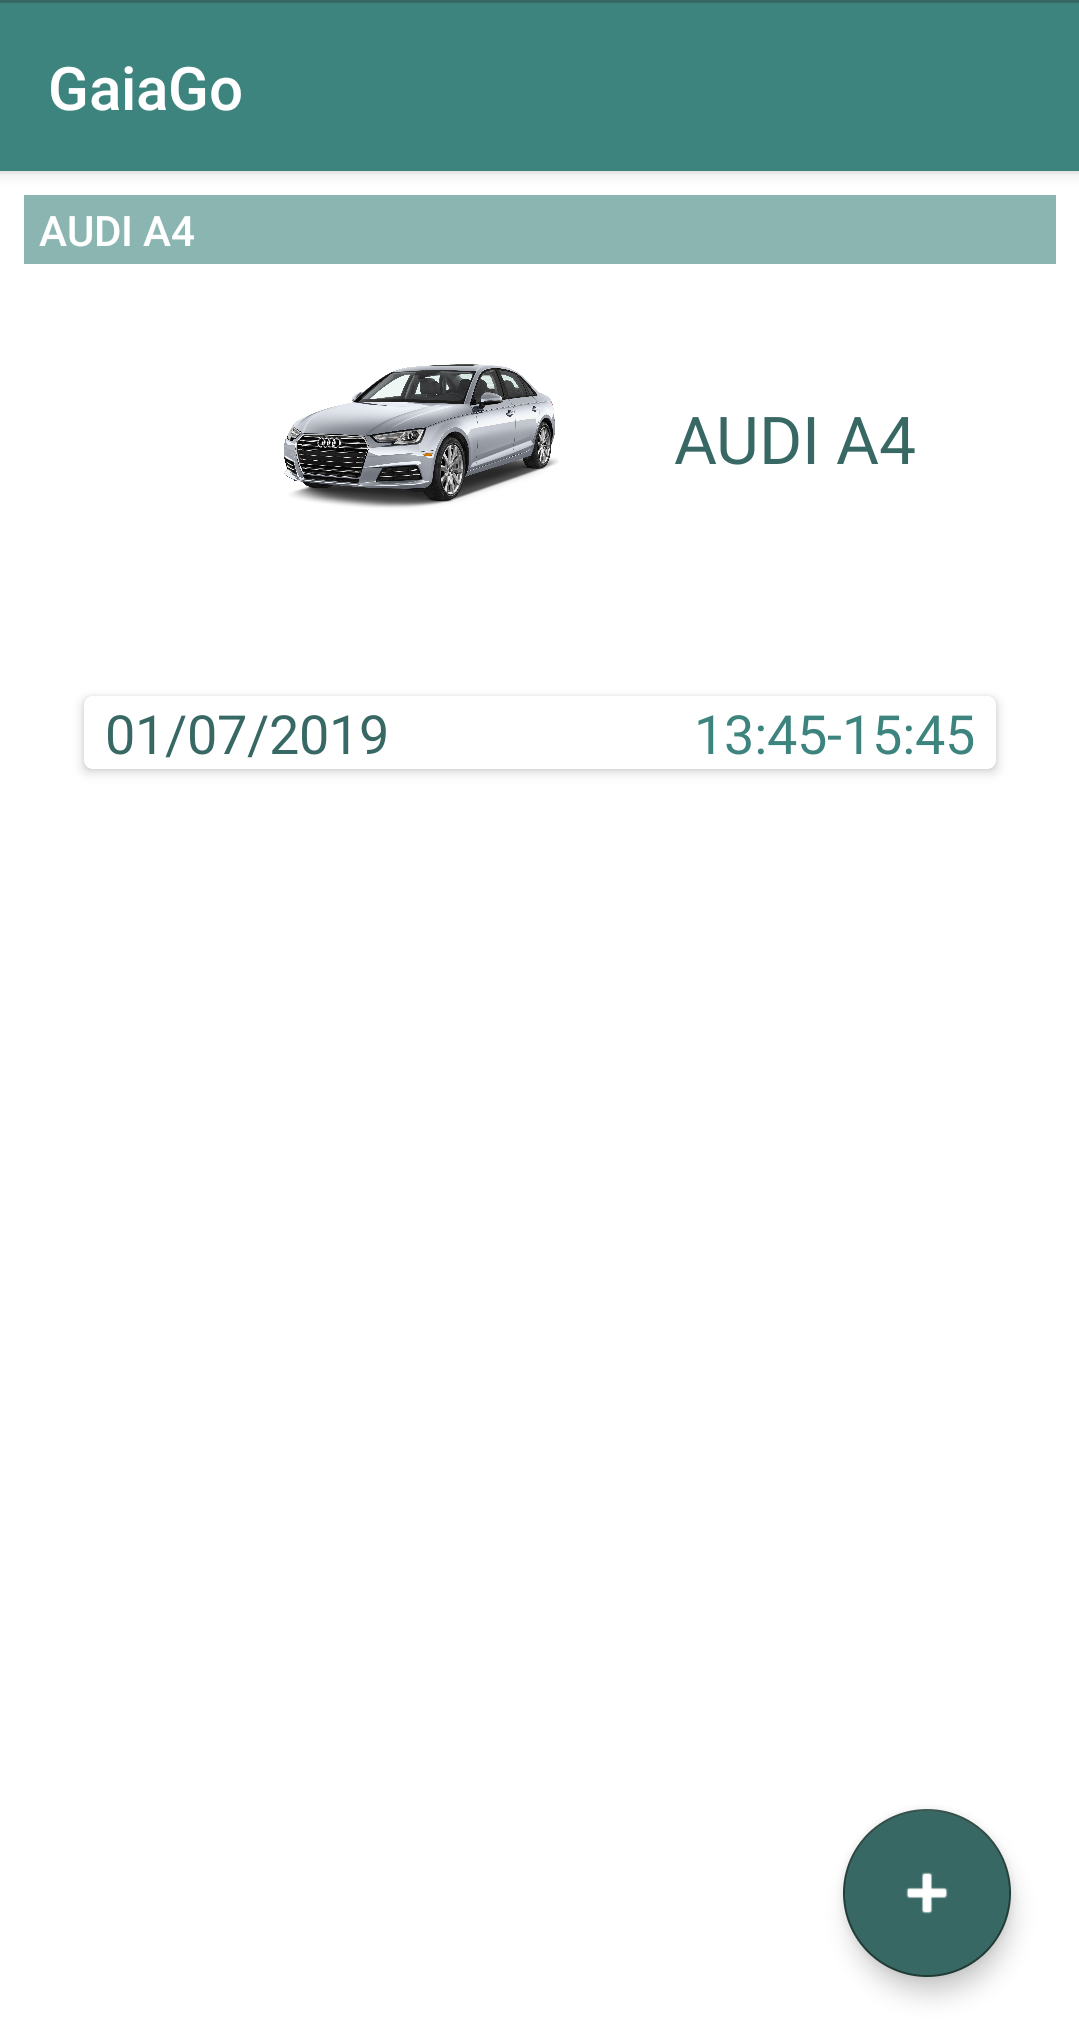
\includegraphics[width=0.5\textwidth]{res/images/disponibilita.png}\\
	\caption{Visualizza disponibilità}
	\label{disponibilità1}
\end{figure}
\pagebreak
Una volta premuto il pulsante si passa all'attività di inserimento dei dati per definire i giorni e la fascia oraria in cui sarà possibile richiedere una prenotazione del veicolo. 
Da questa sezione è possibile accedere alle seguenti funzionalità:
\begin{itemize}
	\item \textbf{Singola}: premendo sul campo "data prenotazione" si avrà accesso ad un calendario per indicare il giorno in cui rendere disponibile il mezzo, "ora di inizio" e "ora di fine" richiedono l'inserimento di una fascia oraria con uno scarto di 15 minuti.
	Le azioni sopracitate sono analoghe alla ricerca di una prenotazione, si rimanda alla sezione \textit{\hyperref[sec:hello]{Ricerca veicolo}} per la spiegazione con annesse figure.
	\begin{figure}[H] 
		\centering 
		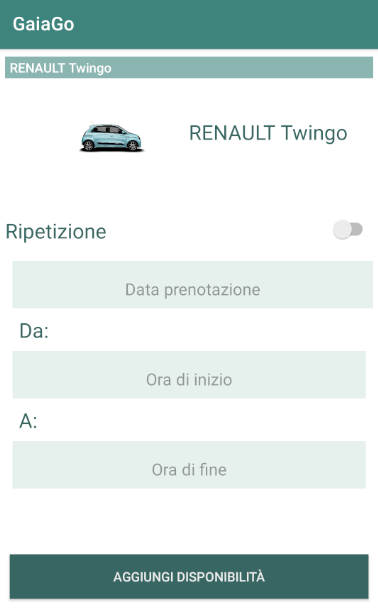
\includegraphics[width=0.5\textwidth]{res/images/aggiungi_disponibilita2.png}\\
		\caption{Inserimento campi singola disponibilità}
		\label{campi disponibilità}
	\end{figure}
	\pagebreak
	\item \textbf{Ripetuta}: da accesso ad un nuovo insieme di campi per poter rendere disponibile il veicolo più volte senza dover inserire manualmente tutti i dati. 
	\begin{figure}[H] 
		\centering 
		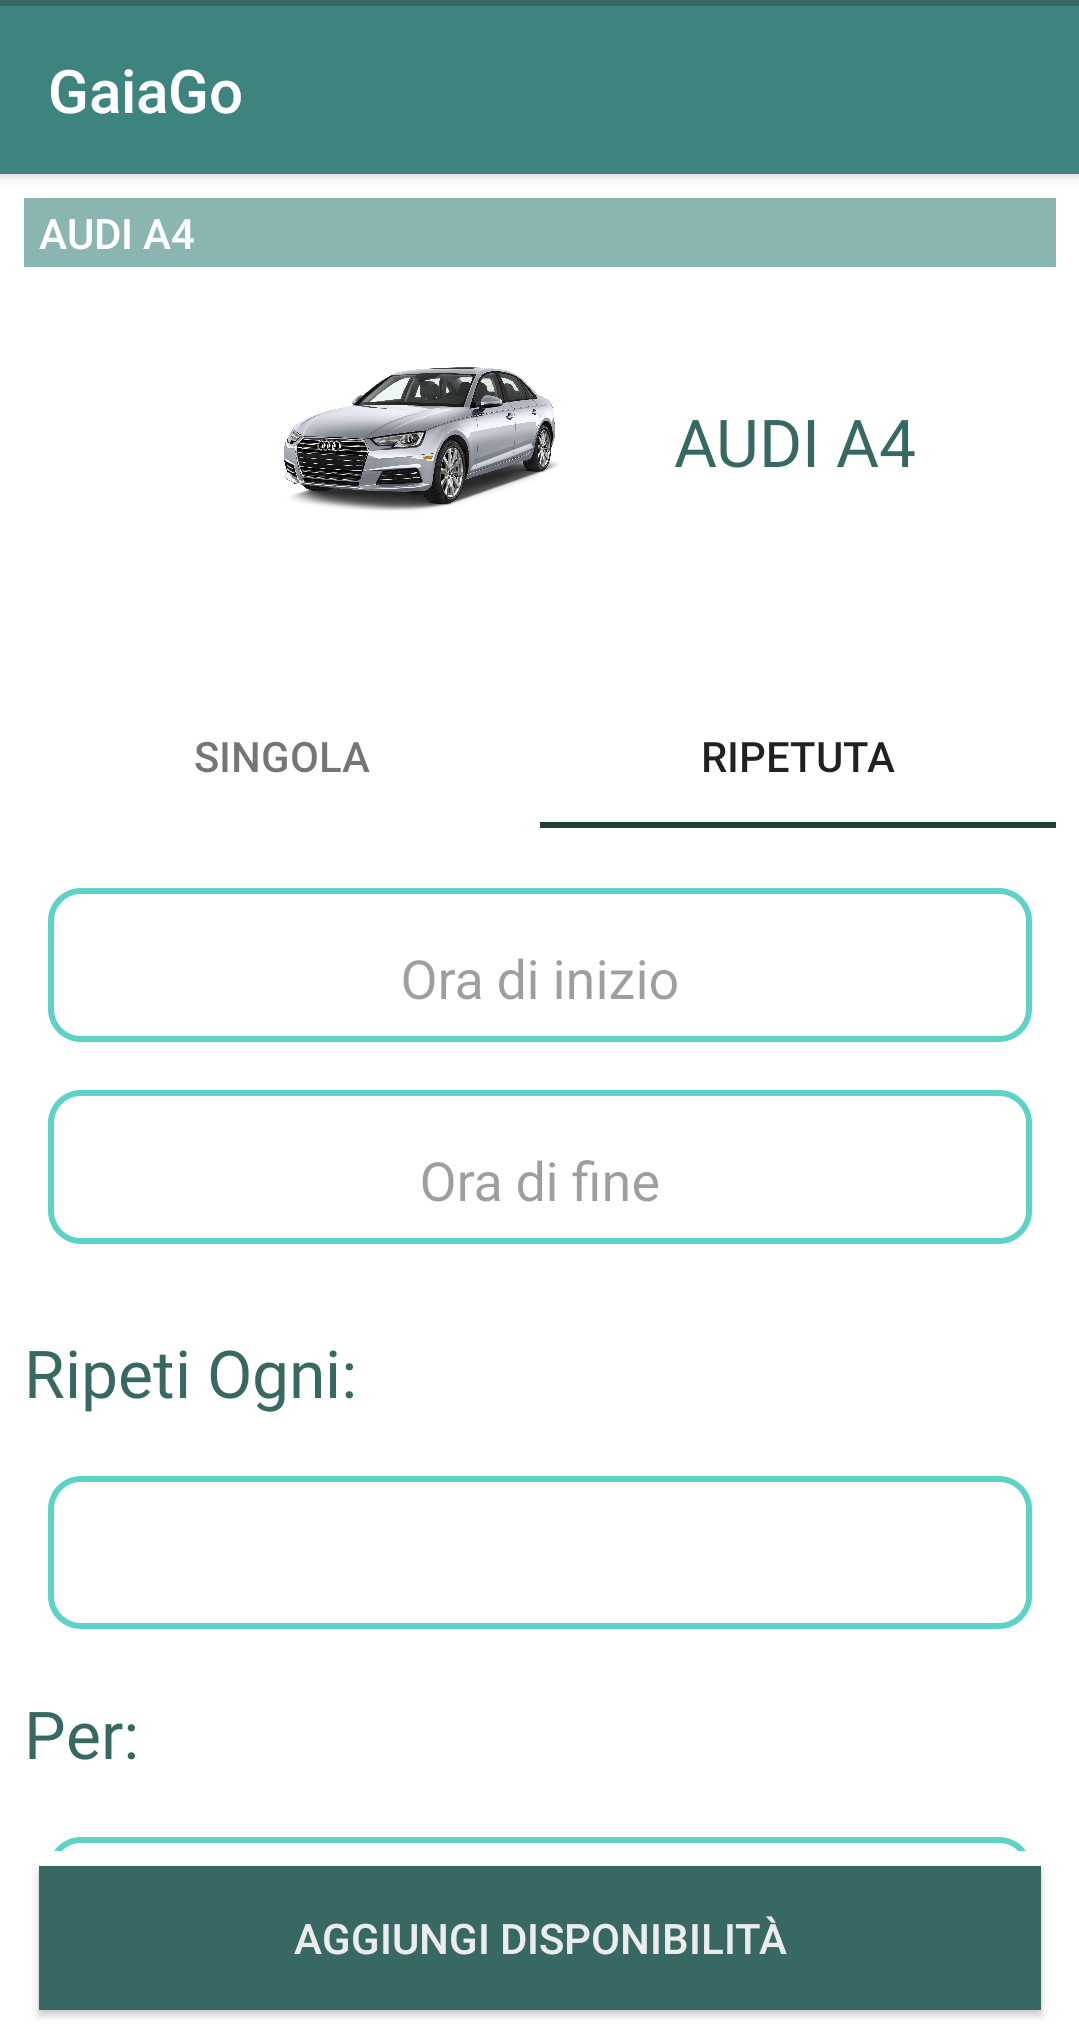
\includegraphics[width=0.5\textwidth]{res/images/aggiungi_disponibilita3.png}\\
		\caption{Inserimento campi ripetuta disponibilità}
		\label{campi disponibilità2}
	\end{figure}
	\pagebreak
	Si presuma che l'utente proprietario voglia rendere prenotabile il proprio mezzo tutti i martedì dalle 10:00 alle 13:00 con questa schermata può farlo una sola volta per più tempo anziché dover inserire la disponibilità singolarmente per ogni volta.
	\begin{figure}[H] 
		\centering 
		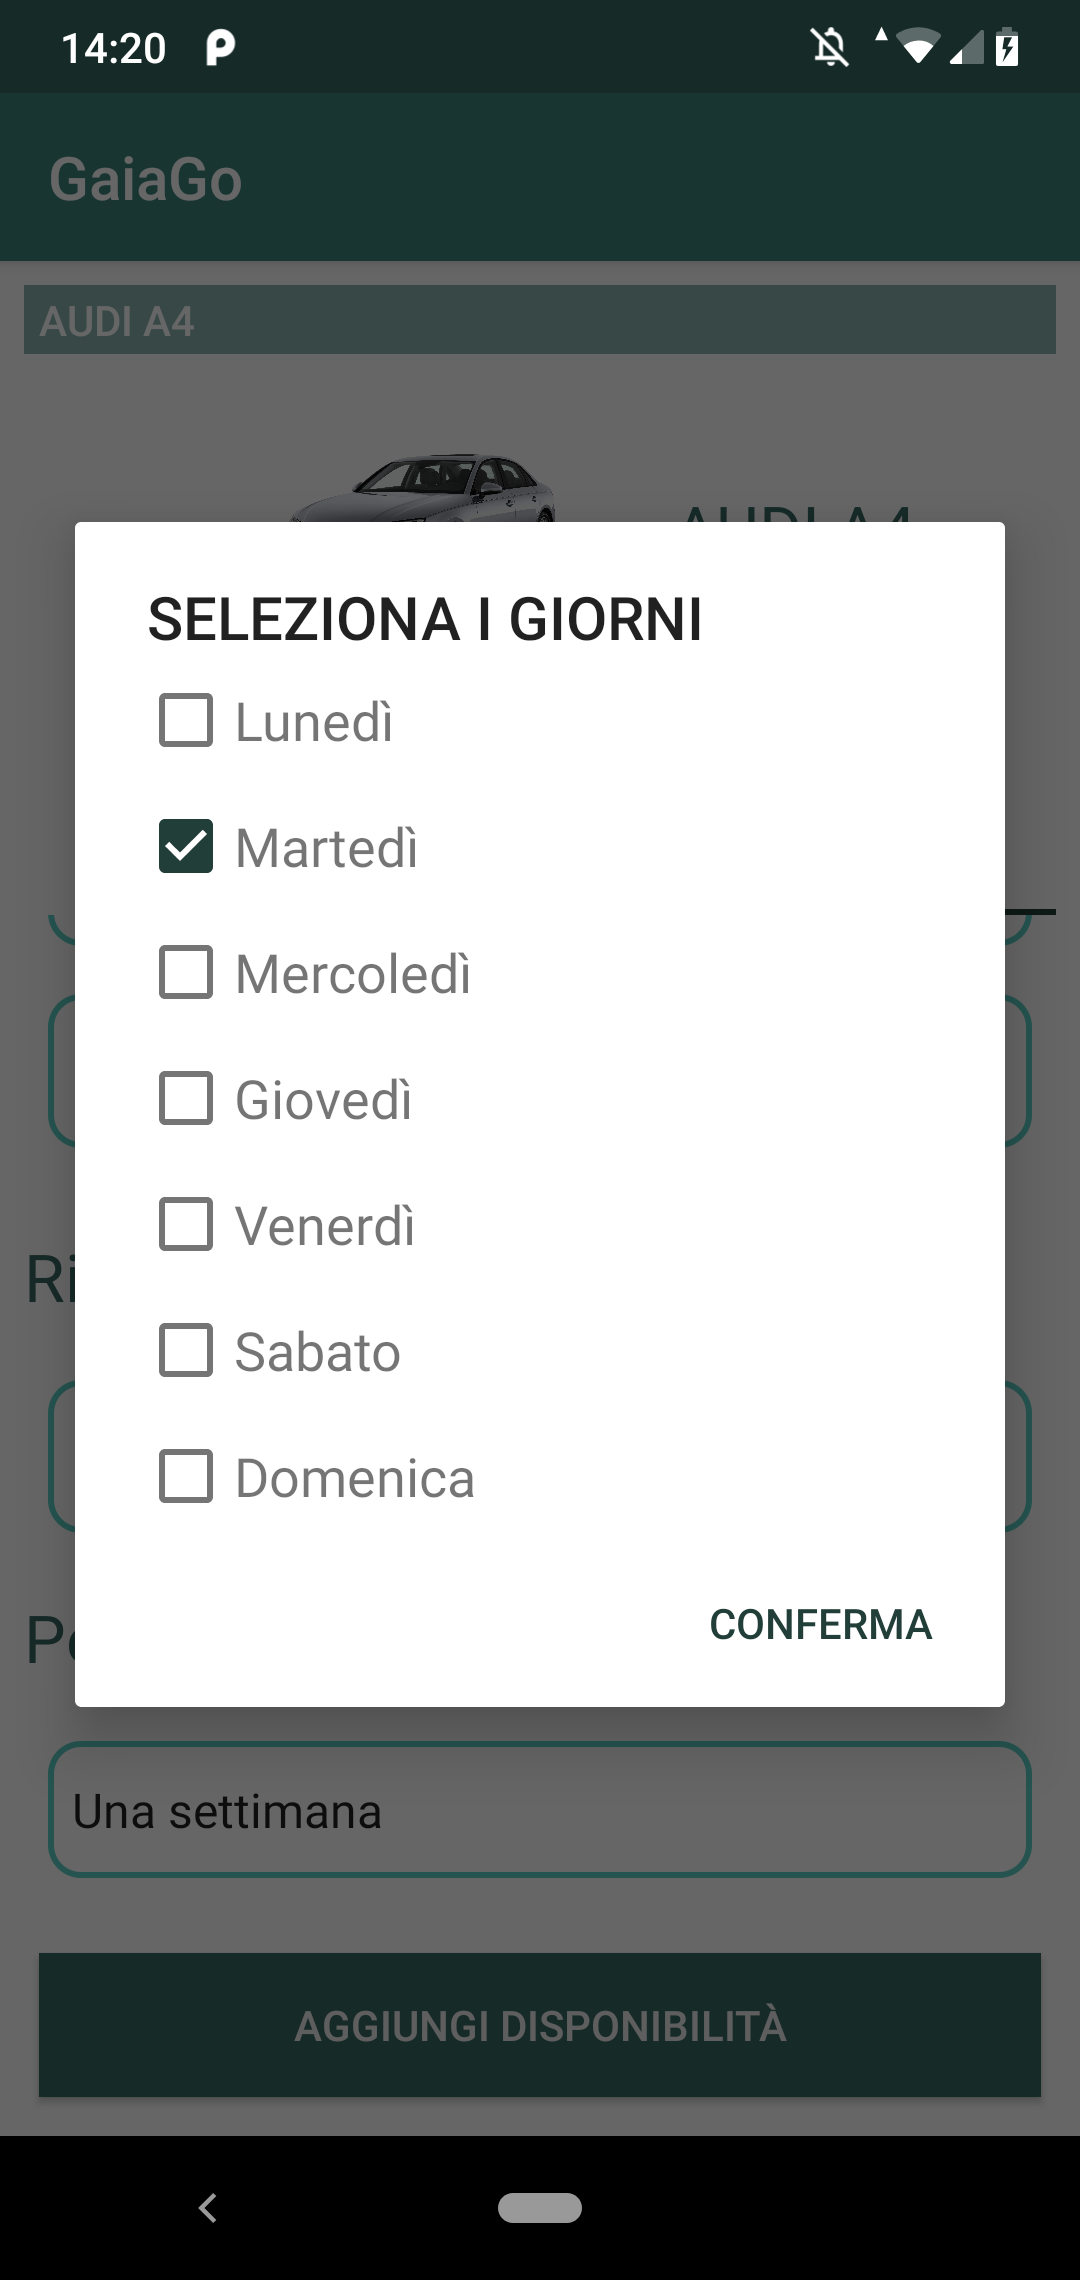
\includegraphics[width=0.5\textwidth]{res/images/aggiungi_disponibilita4.png}\\
		\caption{Inserimento ripetizione giorni settimana}
		\label{disponibilità2}
	\end{figure}
	\begin{figure}[H] 
		\centering 
		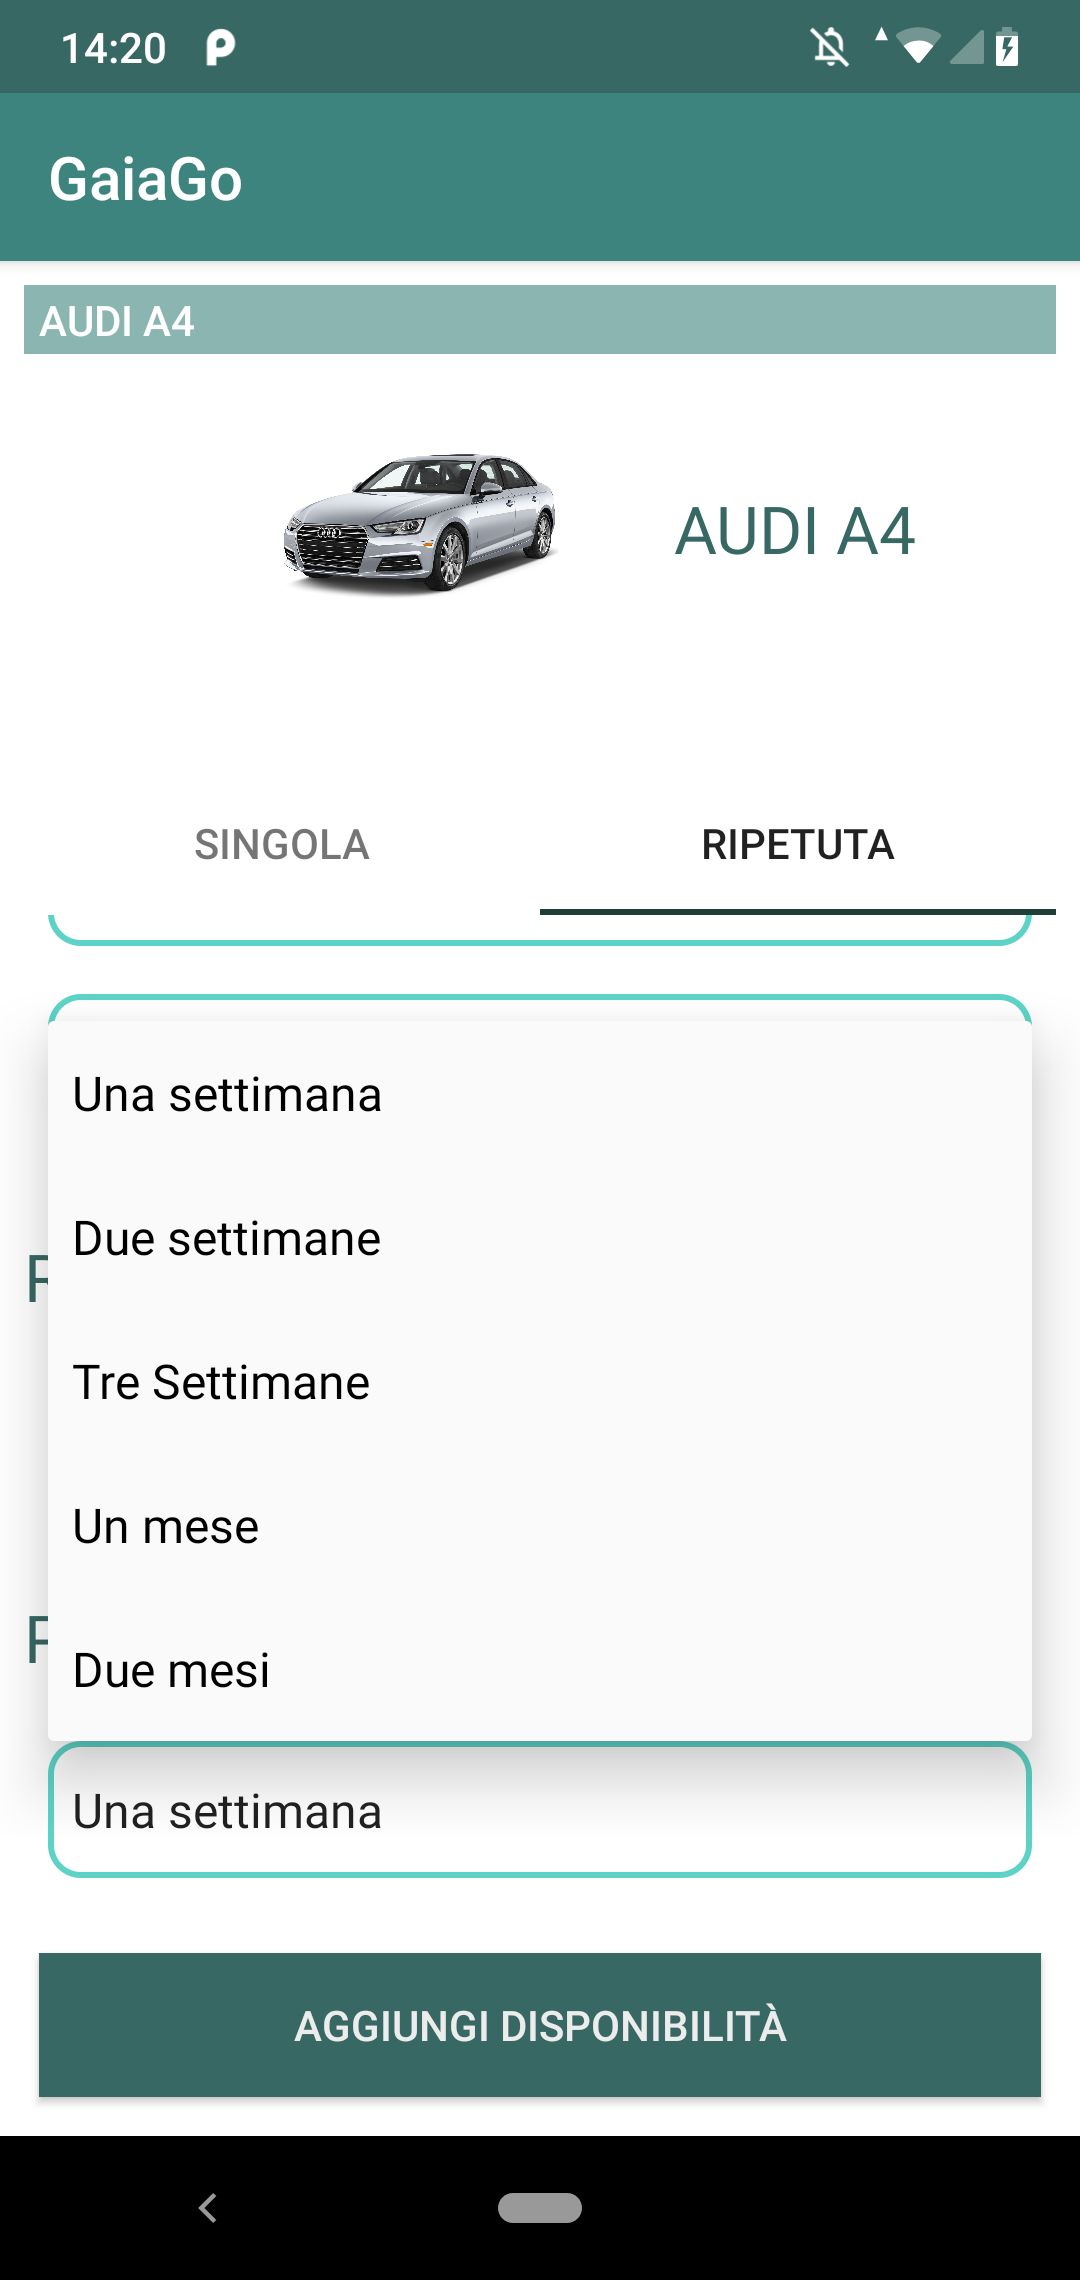
\includegraphics[width=0.5\textwidth]{res/images/aggiungi_disponibilita5.png}\\
		\caption{Inserimento ripetizione quantità di tempo}
		\label{disponibilità3}
	\end{figure}
\end{itemize}
Per concludere l'aggiunta di una disponibilità premere il pulsante "AGGIUNGI DISPONIBILITà".\\
Una volta premuto il pulsante verrà mostrato un pop-up con il seguente messaggio di conferma:
\begin{figure}[H] 
	\centering 
	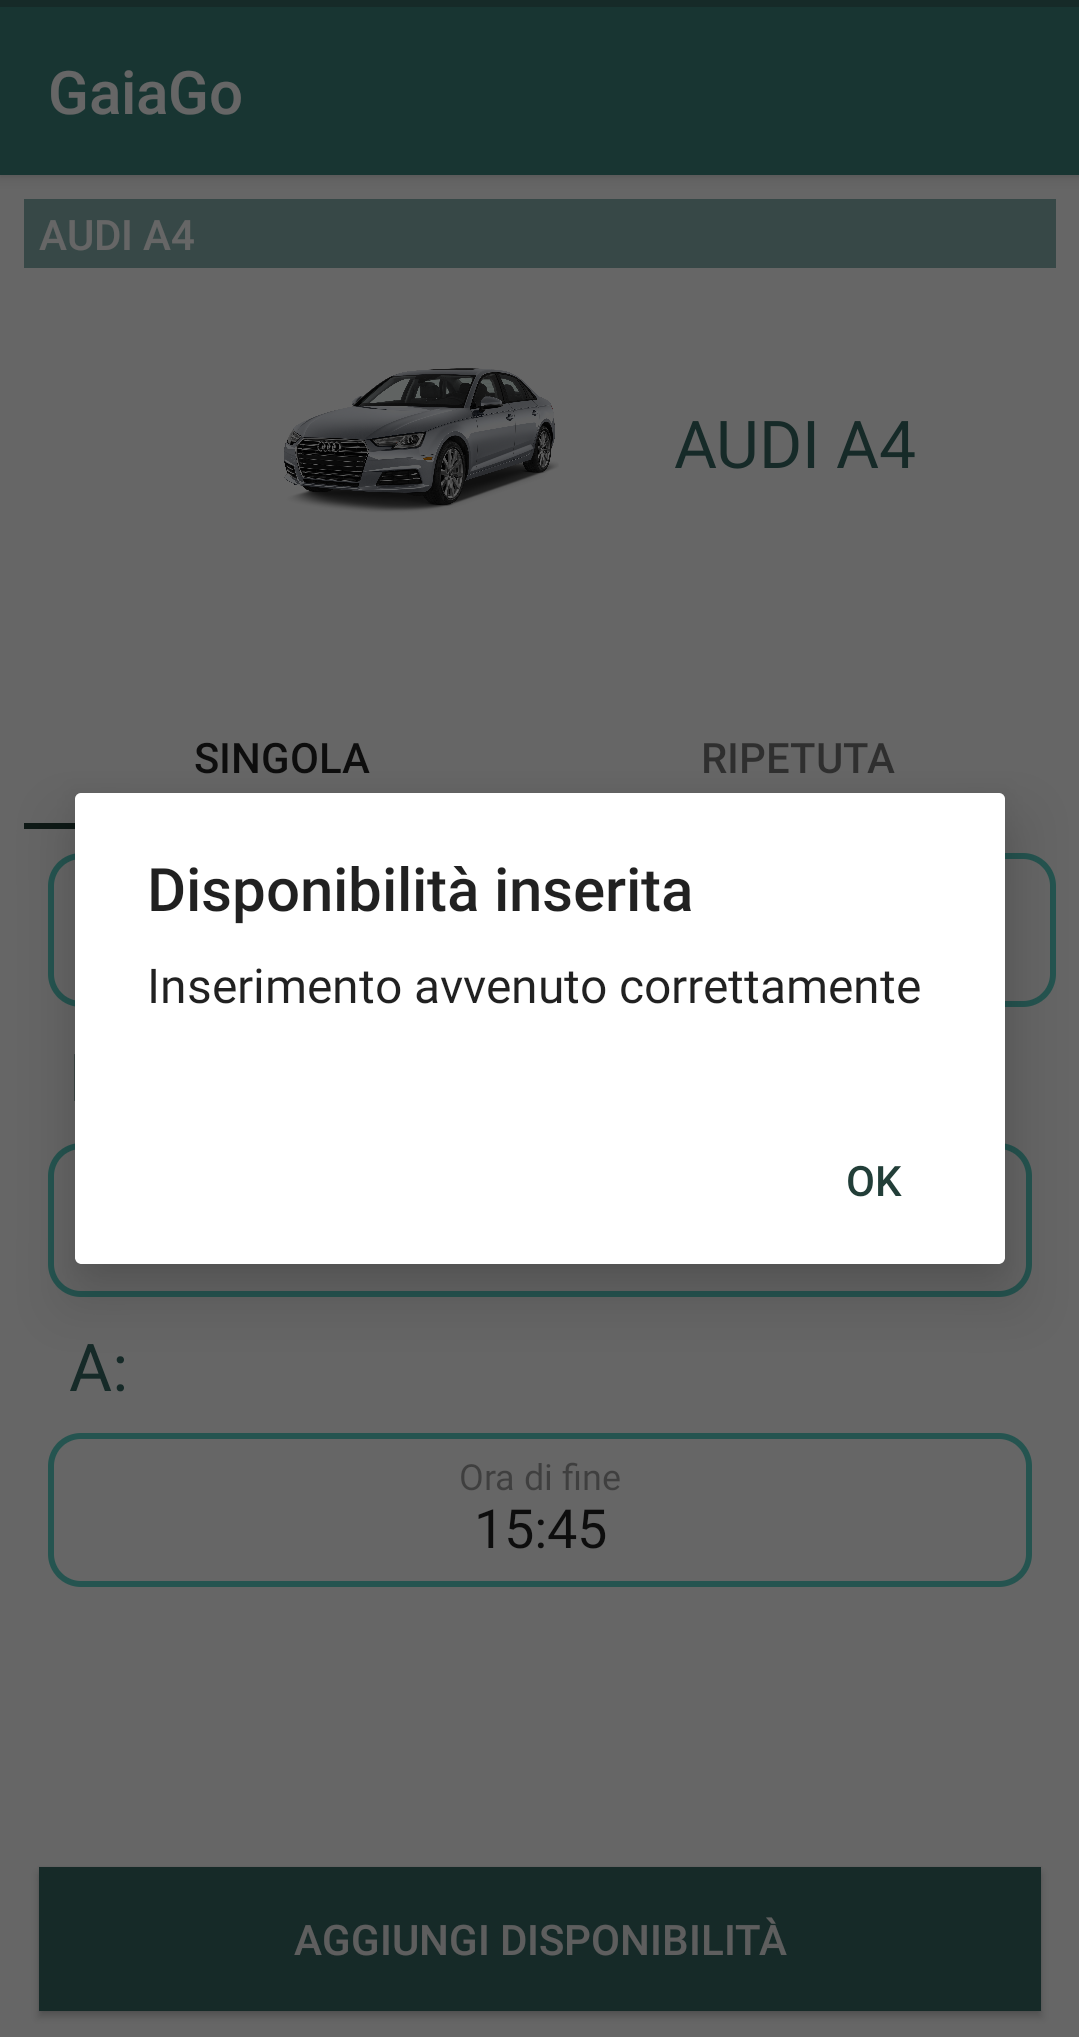
\includegraphics[width=0.5\textwidth]{res/images/conferma_disponibilita.png}\\
	\caption{Conferma rimozione veicolo}
	\label{conferma}
\end{figure}
Premere "OK" per tornare alla schermata di visualizzazione disponibilità. 
\pagebreak

\subsection{Statistiche veicolo}
Nella schermata principale di visualizzazione dei veicoli è possibile, premendo su uno di essi, vedere i dettagli di quest'ultimo e si ha la possibilità di rimuoverlo dall'applicazione, visualizzarne le statistiche oppure di visualizzare le disponibilità aggiunte al veicolo. Una volta presenti nella schermata del veicolo si preme sul pulsante "VISUALIZZA STATISTICHE".
\begin{figure}[H] 
	\centering 
	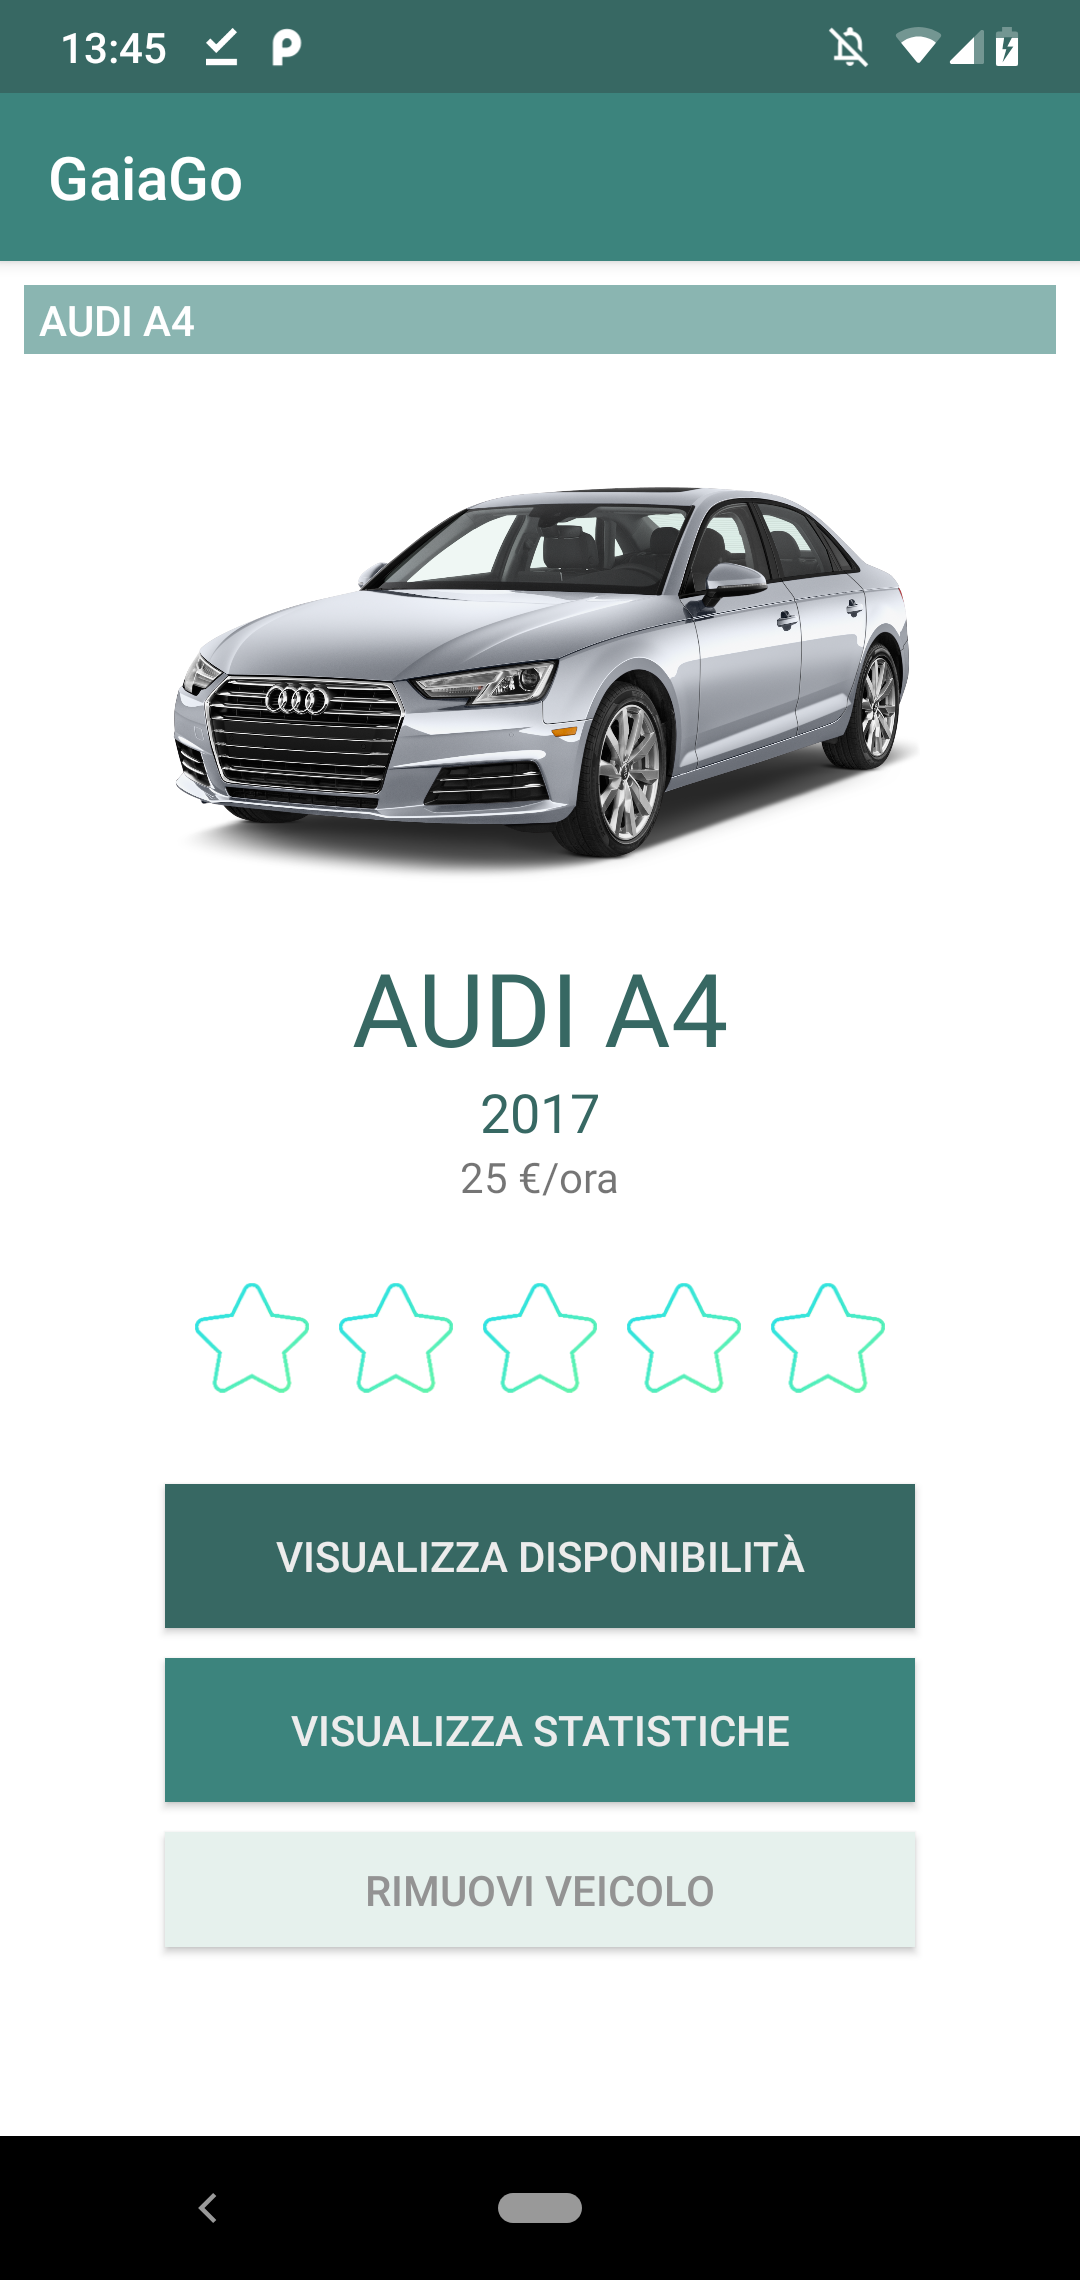
\includegraphics[width=0.5\textwidth]{res/images/visualizza_dettagli.png}\\
	\caption{Visualizza dettagli veicolo}
	\label{statistiche}
\end{figure}
\pagebreak
Una volta premuto il pulsante...
\pagebreak

\subsection{Rimuovi veicolo}
Nella schermata principale di visualizzazione dei veicoli è possibile, premendo su uno di essi, vedere i dettagli di quest'ultimo e si ha la possibilità di rimuoverlo dall'applicazione, visualizzarne le statistiche oppure di visualizzare le disponibilità aggiunte al veicolo. Una volta presenti nella schermata del veicolo si preme sul pulsante "RIMUOVI VEICOLO".
\begin{figure}[H] 
	\centering 
	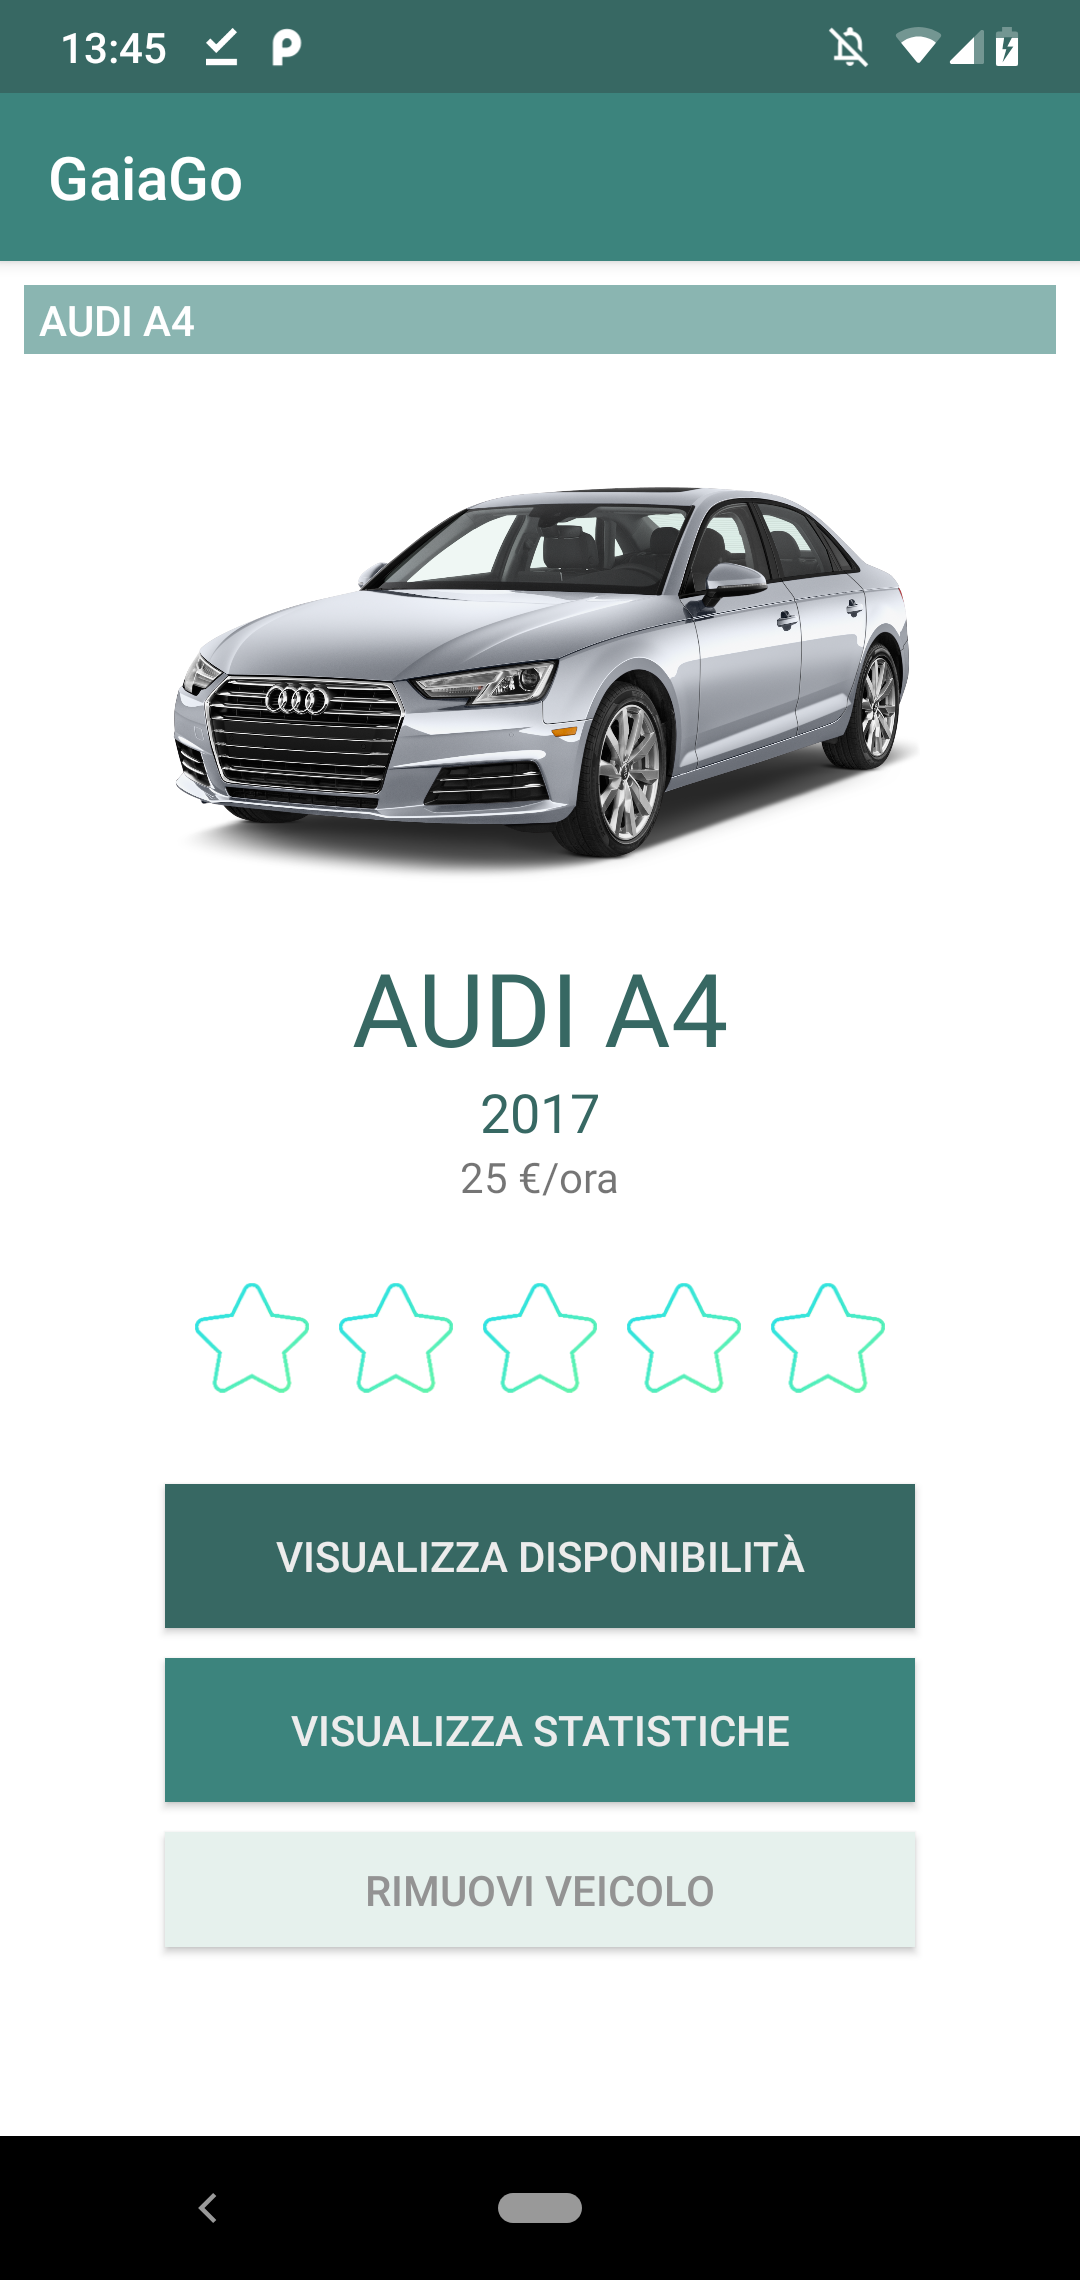
\includegraphics[width=0.5\textwidth]{res/images/visualizza_dettagli.png}\\
	\caption{Visualizza dettagli veicolo}
	\label{rimozione}
\end{figure}
\pagebreak
Una volta premuto il pulsante verrà mostrato un pop-up con la seguente richiesta:
\begin{figure}[H] 
	\centering 
	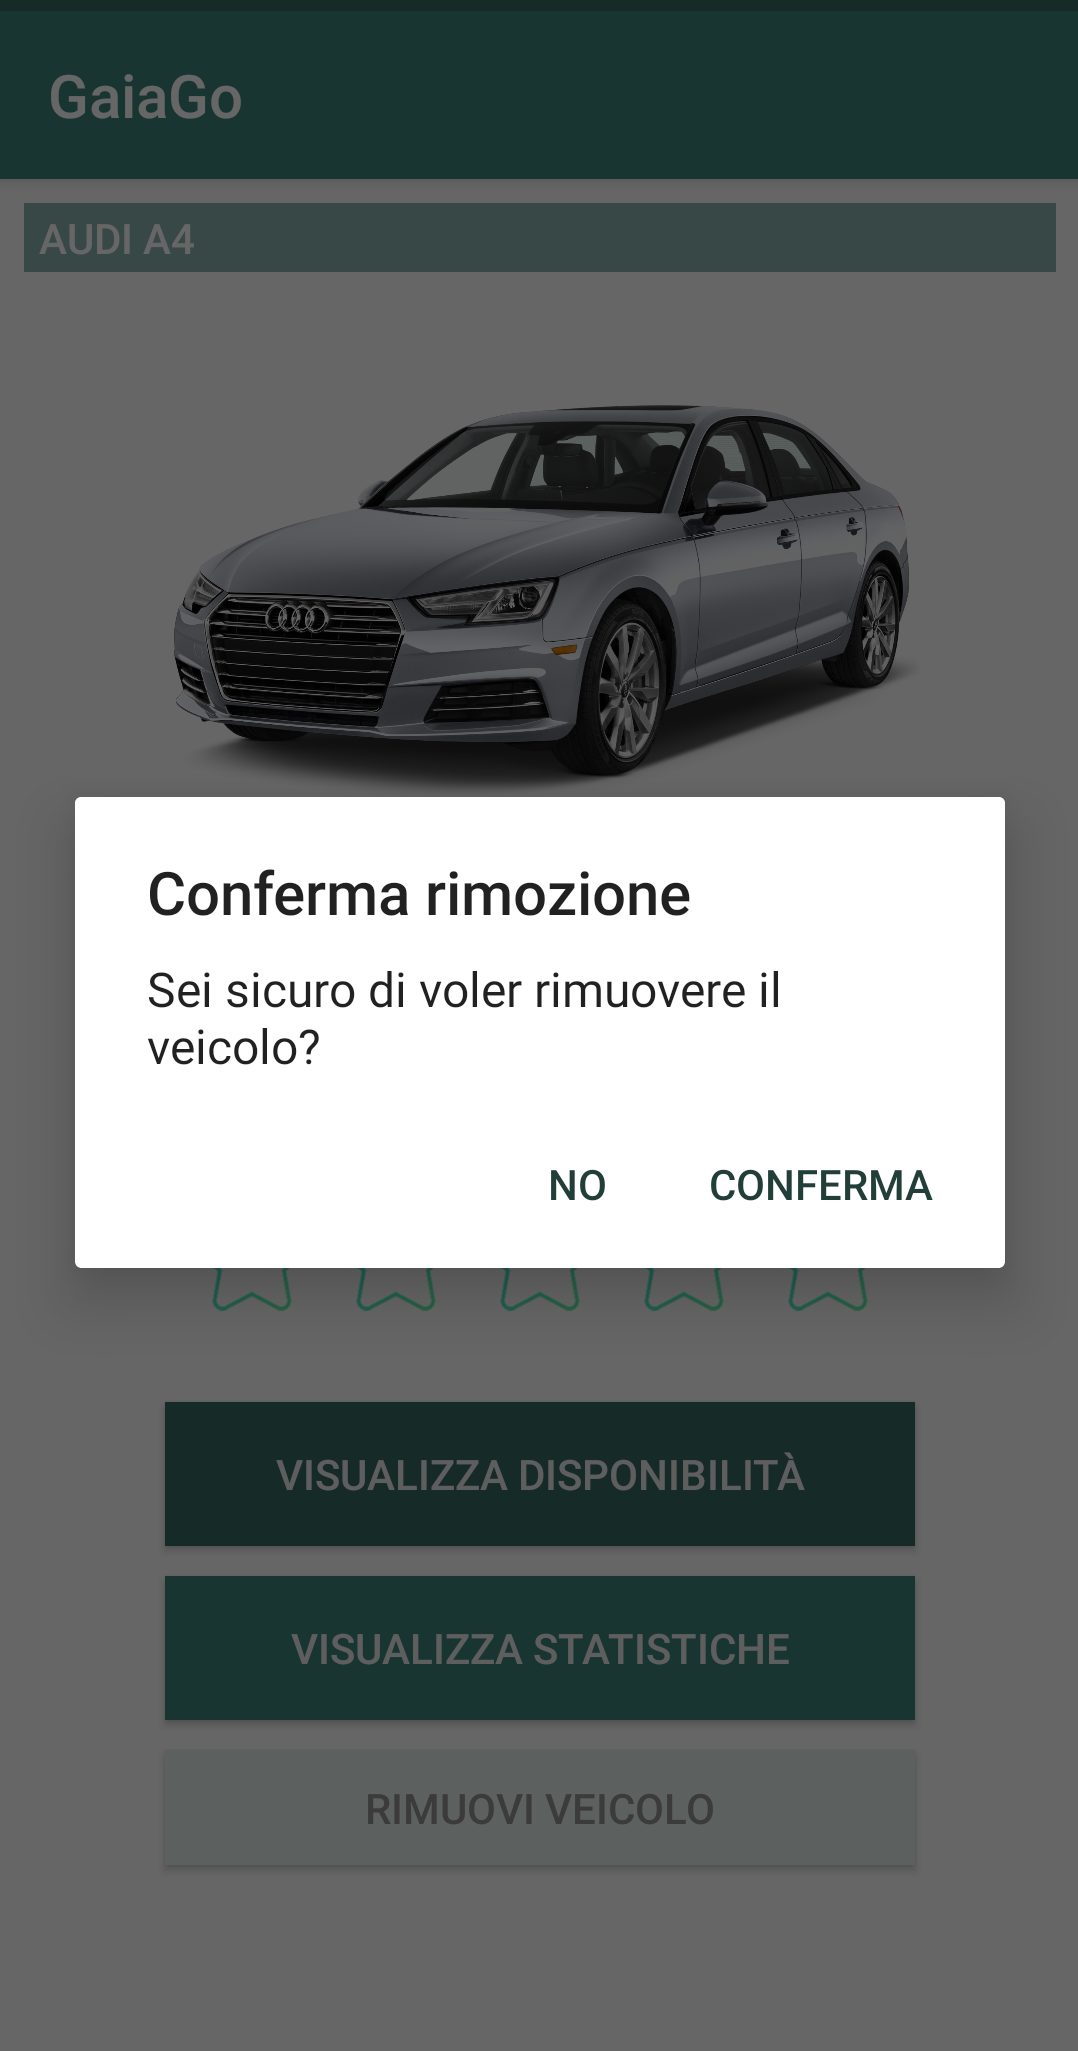
\includegraphics[width=0.5\textwidth]{res/images/rimozione_veicolo.png}\\
	\caption{Conferma rimozione veicolo}
	\label{rimozione1}
\end{figure}
Per concludere la rimozione si prema il pulsante "CONFERMA" altrimenti si prema "NO".
\pagebreak

\subsection{Ricerca veicolo}
\label{ricerca0}
Per effettuare una prenotazione è necessario ricercare i veicoli resi disponibili dagli altri utenti. Per fare ciò da una delle schermate principali si clicca il pulsante sulla barra di navigazione avente una lente d'ingrandimento stilizzata. Una volta premuto si aprirà l'attività principale di ricerca. Il bottone della barra di navigazione presenta ora una scritta "Cerca" a conferma di ciò.
  \begin{figure}[H] 
 	\centering 
 	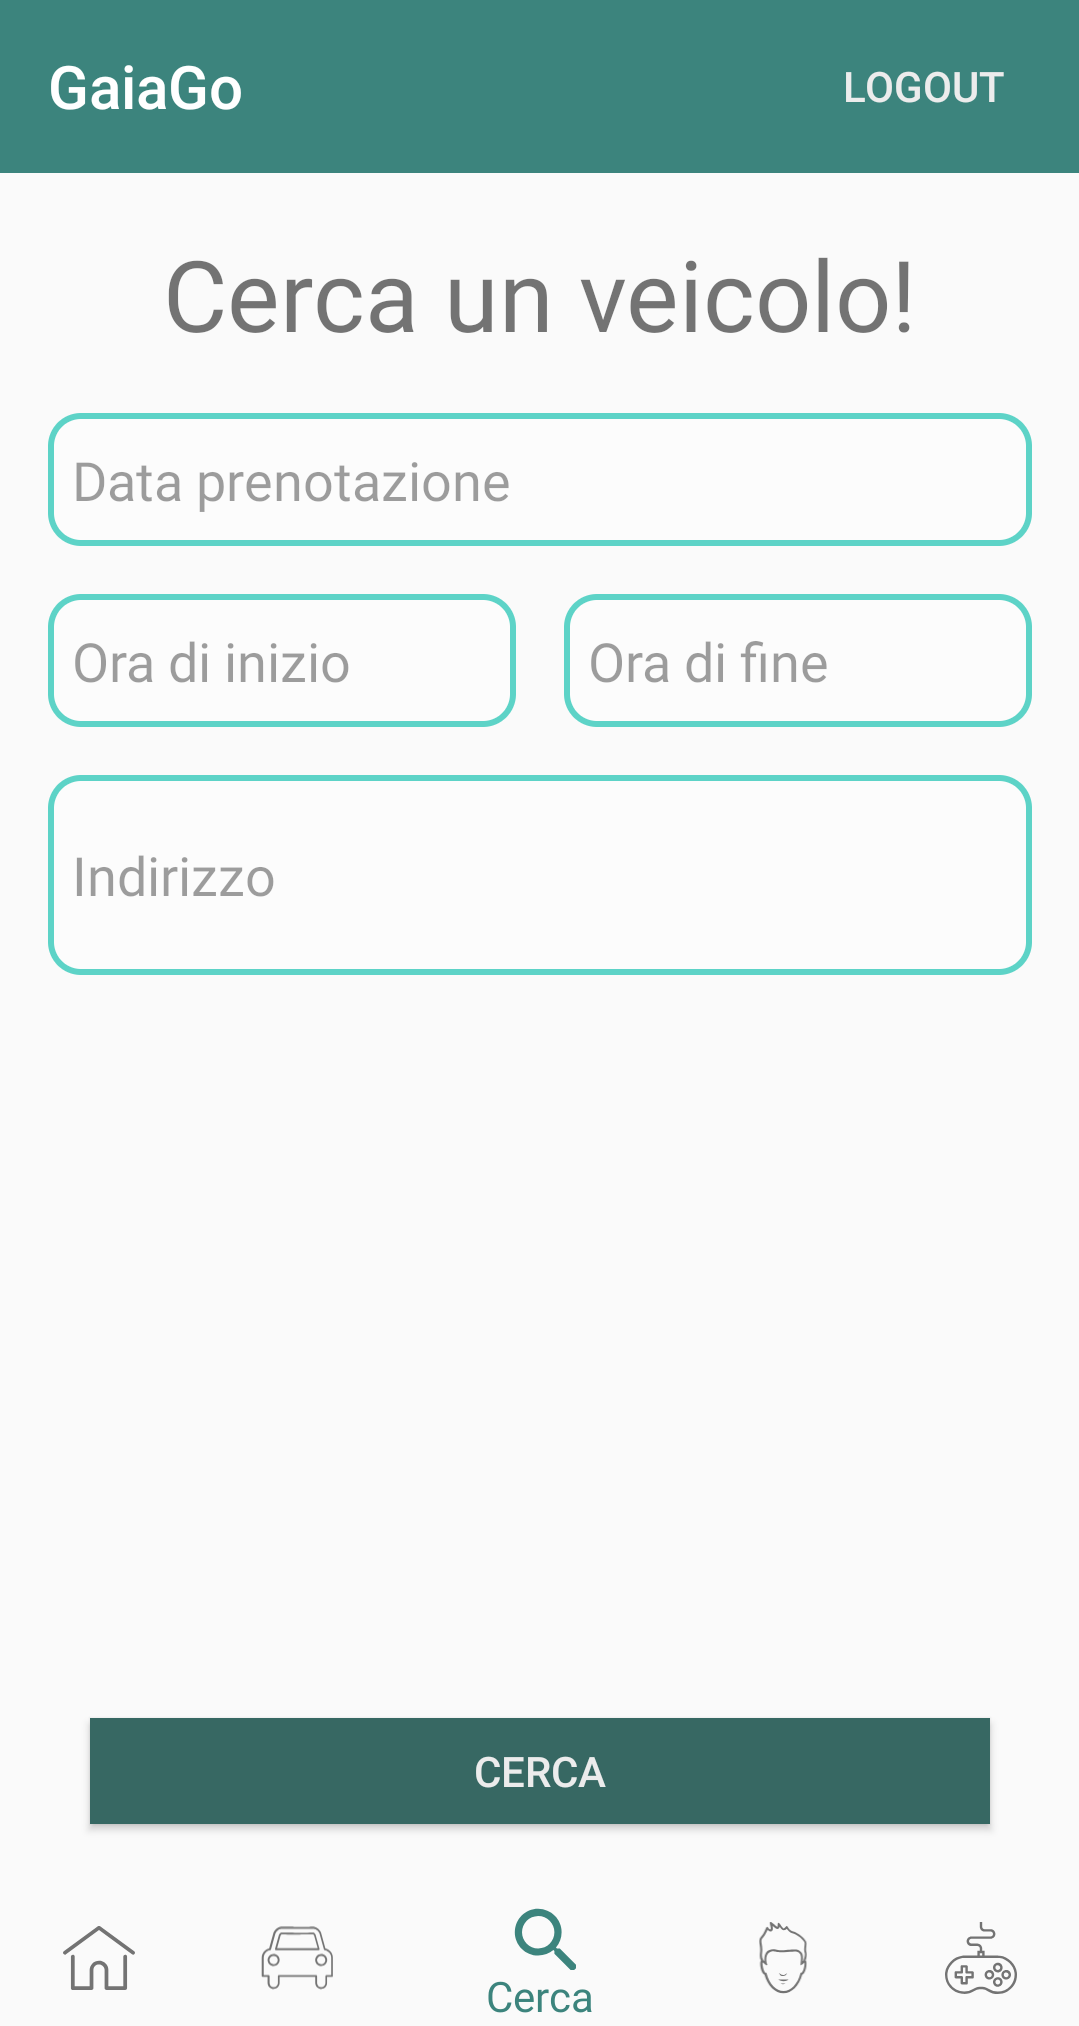
\includegraphics[width=0.5\textwidth]{res/images/cerca_veicolo.png}\\
 	\caption{Activity di ricerca veicolo}
 	\label{ricerca}
 \end{figure}
\pagebreak

Per effettuare una ricerca è necessario compilare tutti i campi richiesti:
\begin{itemize}
	\item \textbf{data prenotazione}: è richiesto il giorno in cui si intende effettuare la prenotazione, per fare ciò si preme sull'editor di testo avente il placeholder\glosp "Data prenotazione" in grigio chiaro. Compare un calendario nel quale si va a selezionare il giorno desiderato;
	 \begin{figure}[H] 
	 	\centering 
	 	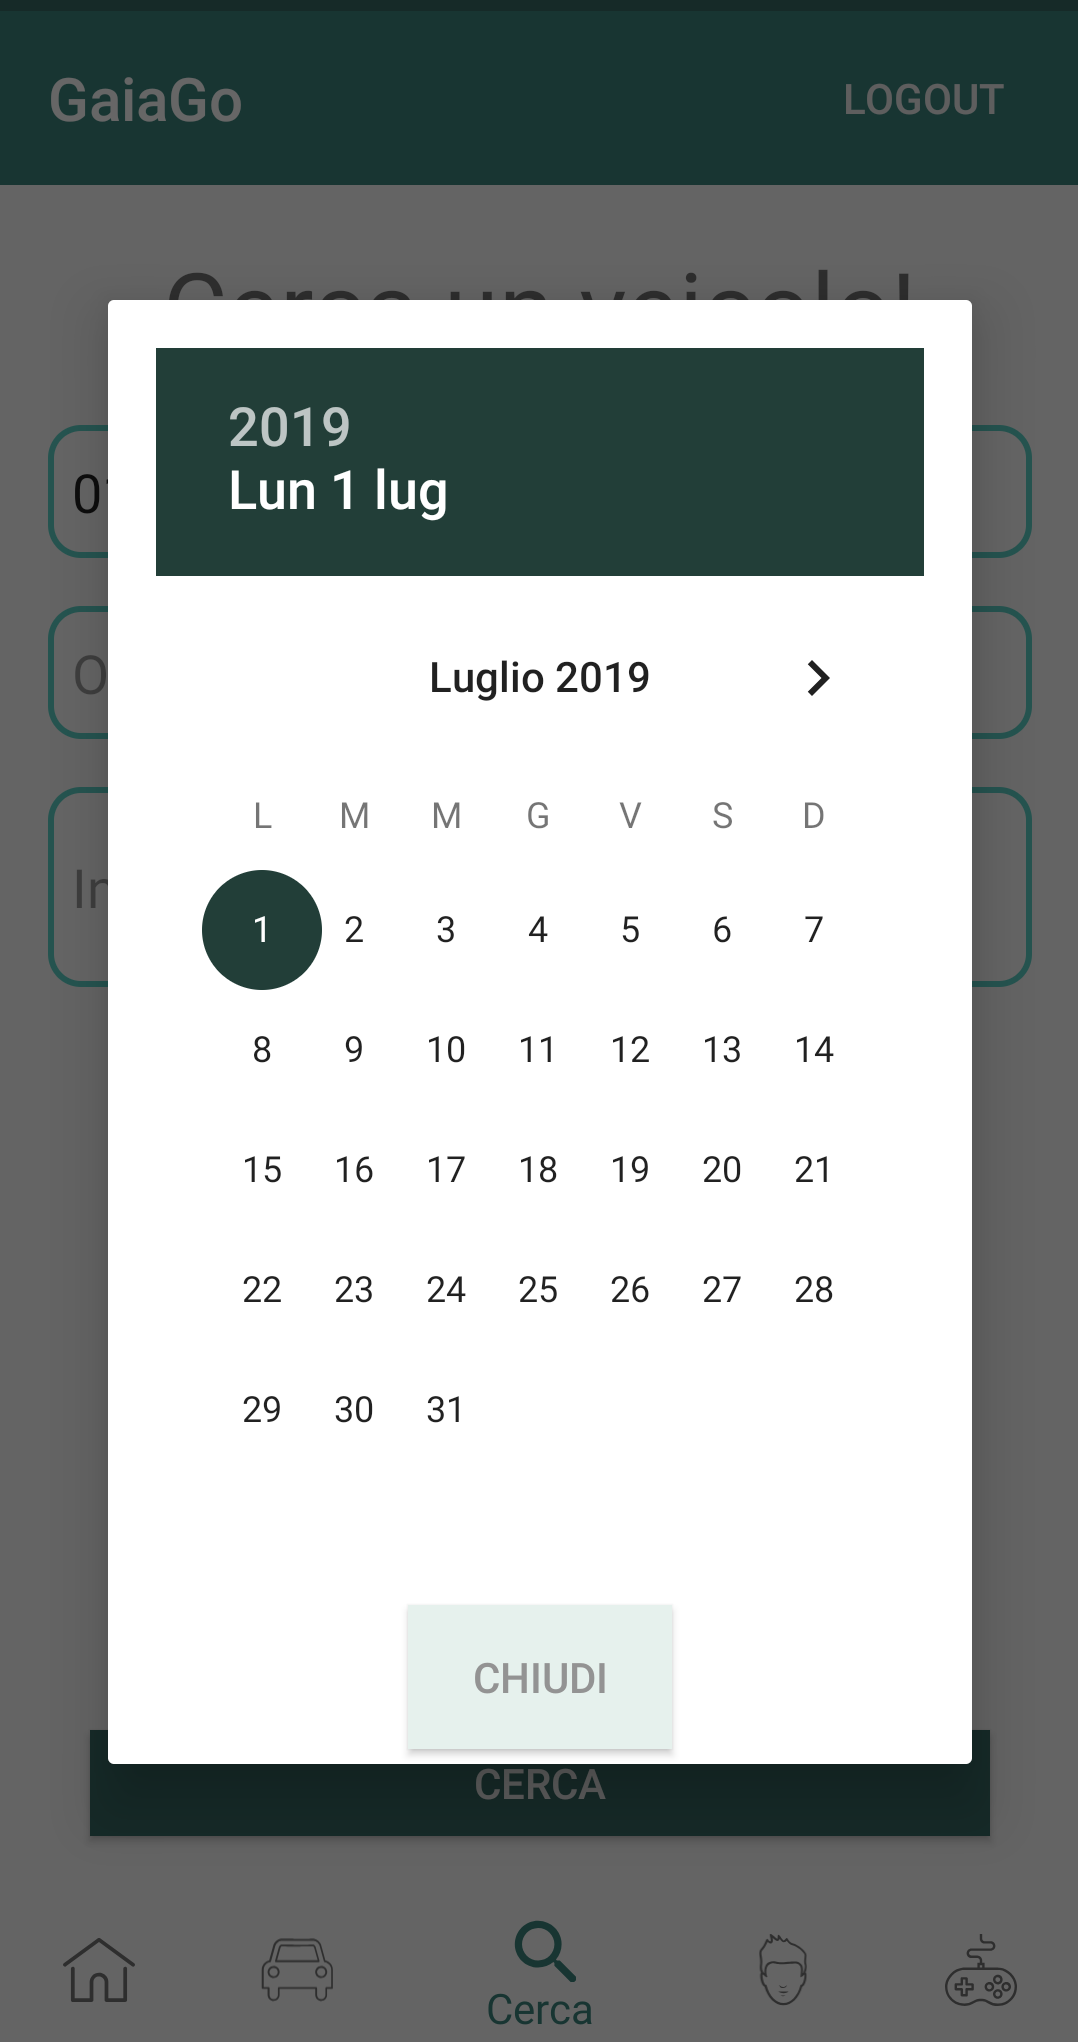
\includegraphics[width=0.5\textwidth]{res/images/data_prenotazione.png}\\
	 	\caption{Data prenotazione}
	 	\label{data}
	 \end{figure}
 \pagebreak
 
 \item \textbf{ora di inizio/fine}: è necessario inserire la fascia oraria nella quale si intende prenotare il veicolo, per fare ciò sono disponibili due campi compilabili "Ora di inizio" e "Ora di fine". Una volta cliccati presentano gli orari da scegliere con una sensibilità di 15 minuti;
  \begin{figure}[H] 
 	\centering 
 	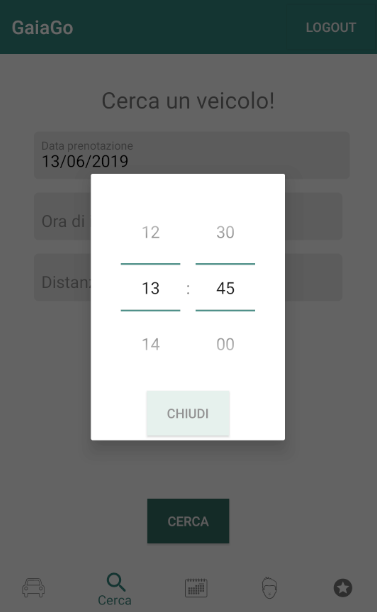
\includegraphics[width=0.5\textwidth]{res/images/ora_inizio.png}\\
 	\caption{Ora prenotazione}
 	\label{ora}
 \end{figure}
 
 \item \textbf{indirizzo}: in questa sezione si inserisce l'indirizzo dove si trova il proprio veicolo, l'indirizzo è geo-localizzato grazie all'uso di un tool\glosp offerto da \textit{Google} il quale ci permette in seguito di ricercare i veicoli in base alla loro posizione sulla mappa. Anche qui è presente l'auto-completamento quindi possono essere inseriti solo indirizzi validi altrimenti non sarà possibile localizzare la reale posizione del veicolo;
\end{itemize}
\pagebreak

Dopo aver compilato tutti i campi si preme il bottone "CERCA" di colore verde e si aprirà la seguente schermata.\\
Da questa sezione è possibile accedere alle seguenti funzionalità:
\begin{itemize}
	\item \textbf{Lista}: vengono mostrate tutti i veicoli disponibili secondo i criteri di ricerca inseriti;
	\begin{figure}[H] 
		\centering 
		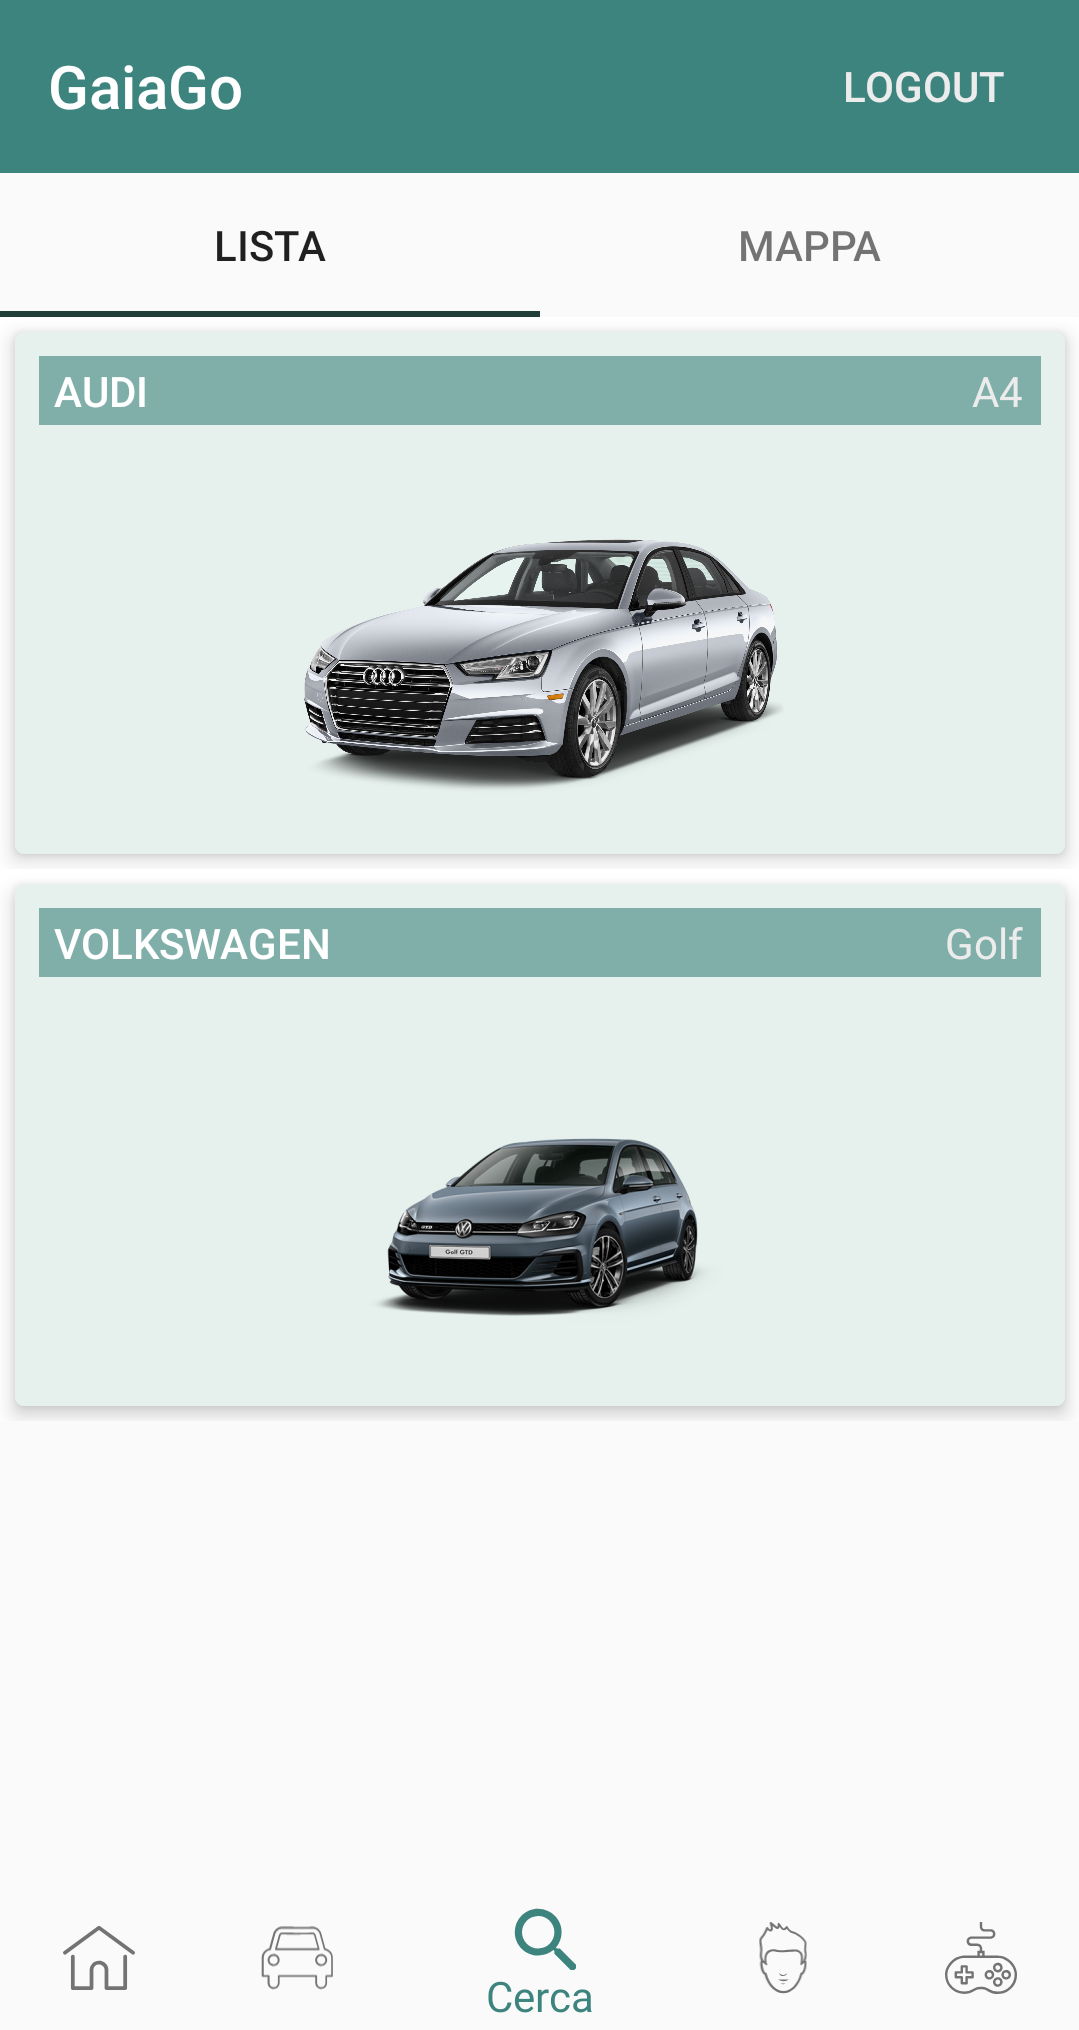
\includegraphics[width=0.5\textwidth]{res/images/ricerca_conclusa.png}\\
		\caption{Ricerca conclusa con una lista}
		\label{lista}
	\end{figure}
	\pagebreak
	\item \textbf{Mappa}: da qui si possono vedere i veicoli posizionati in una mappa in base alla nostra posizione.
	\begin{figure}[H] 
		\centering 
		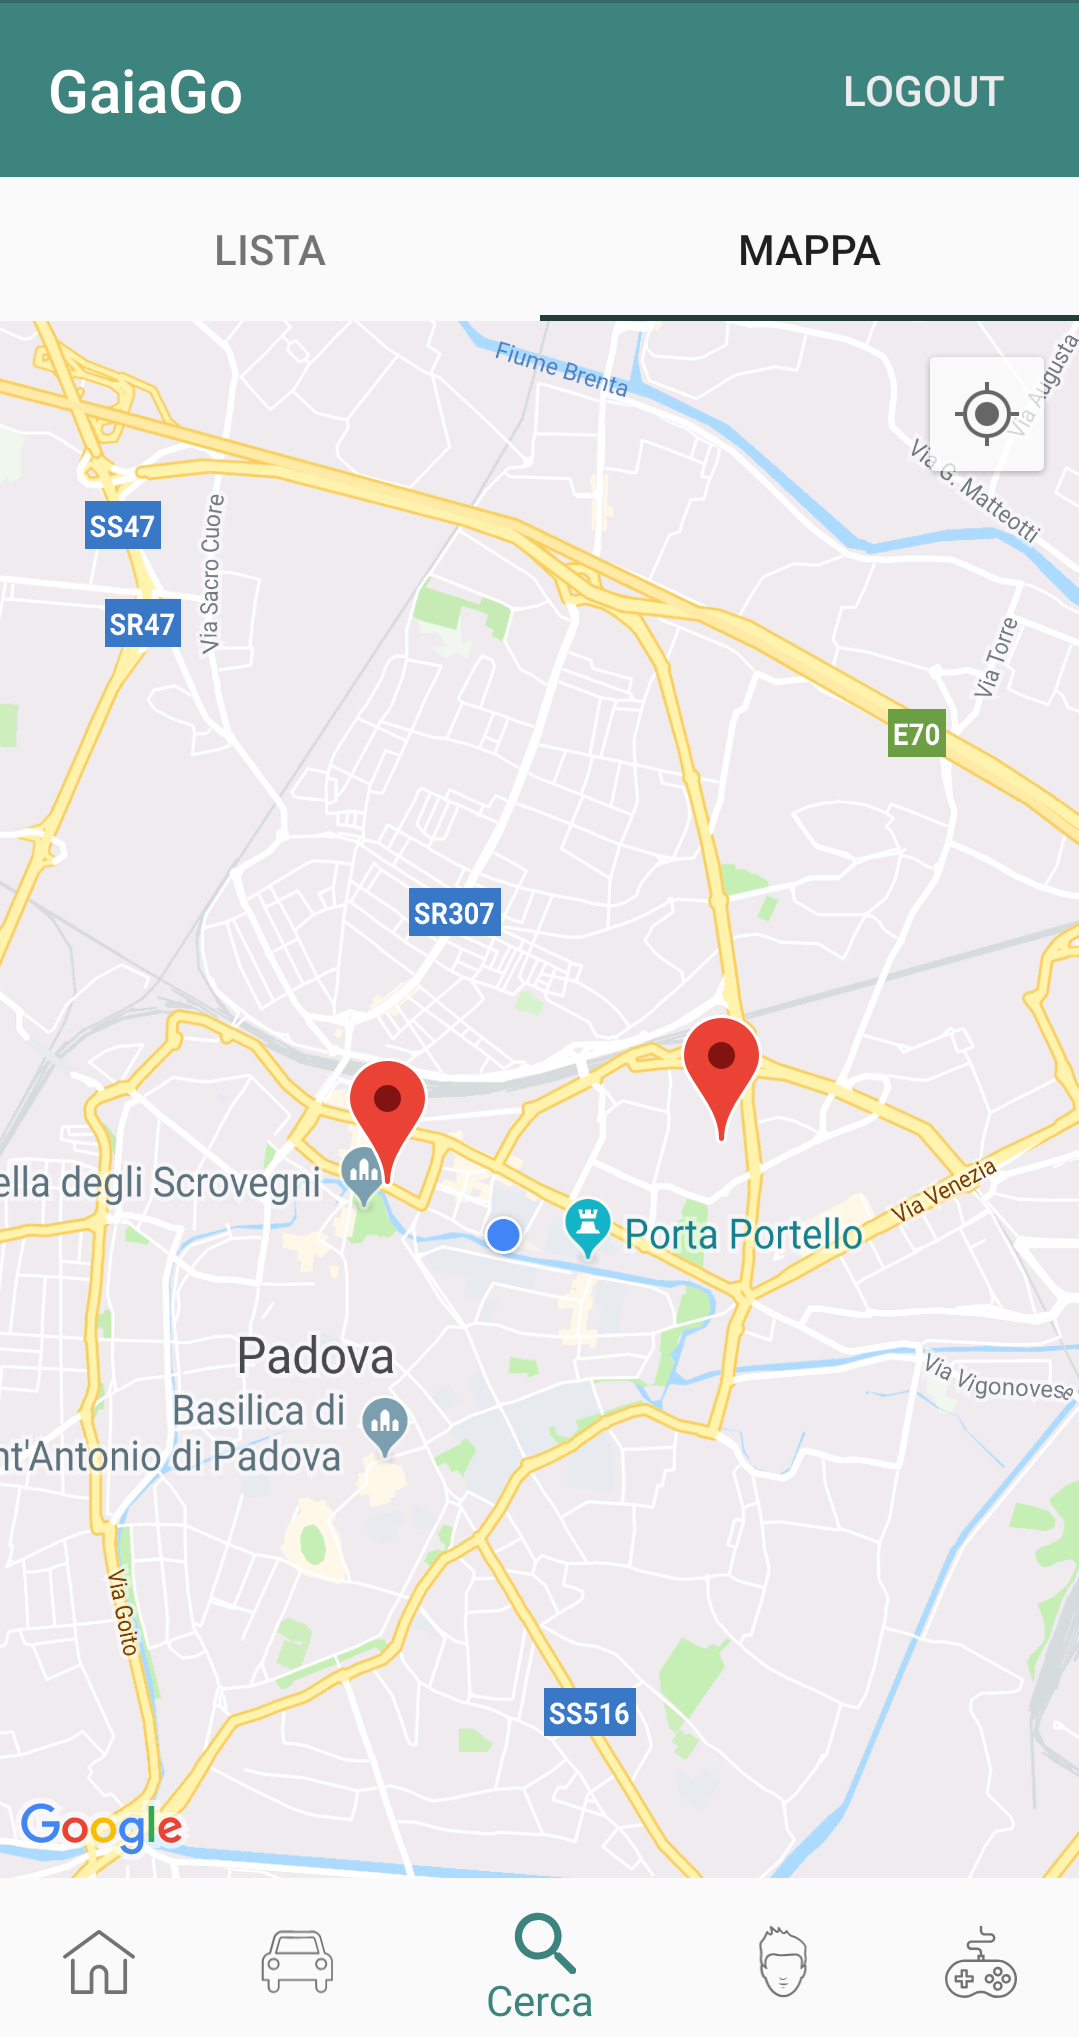
\includegraphics[width=0.5\textwidth]{res/images/mapparicerca.png}\\
		\caption{Ricerca conclusa con una mappa}
		\label{mappa}
	\end{figure}
	\pagebreak
	selezionando uno dei maker\glosp rossi è possibile passare alla schermata di visualizzazione premendo il tasto "VISUALIZZA" oppure "CHIUDI" per chiudere il marker.
	\begin{figure}[H] 
		\centering 
		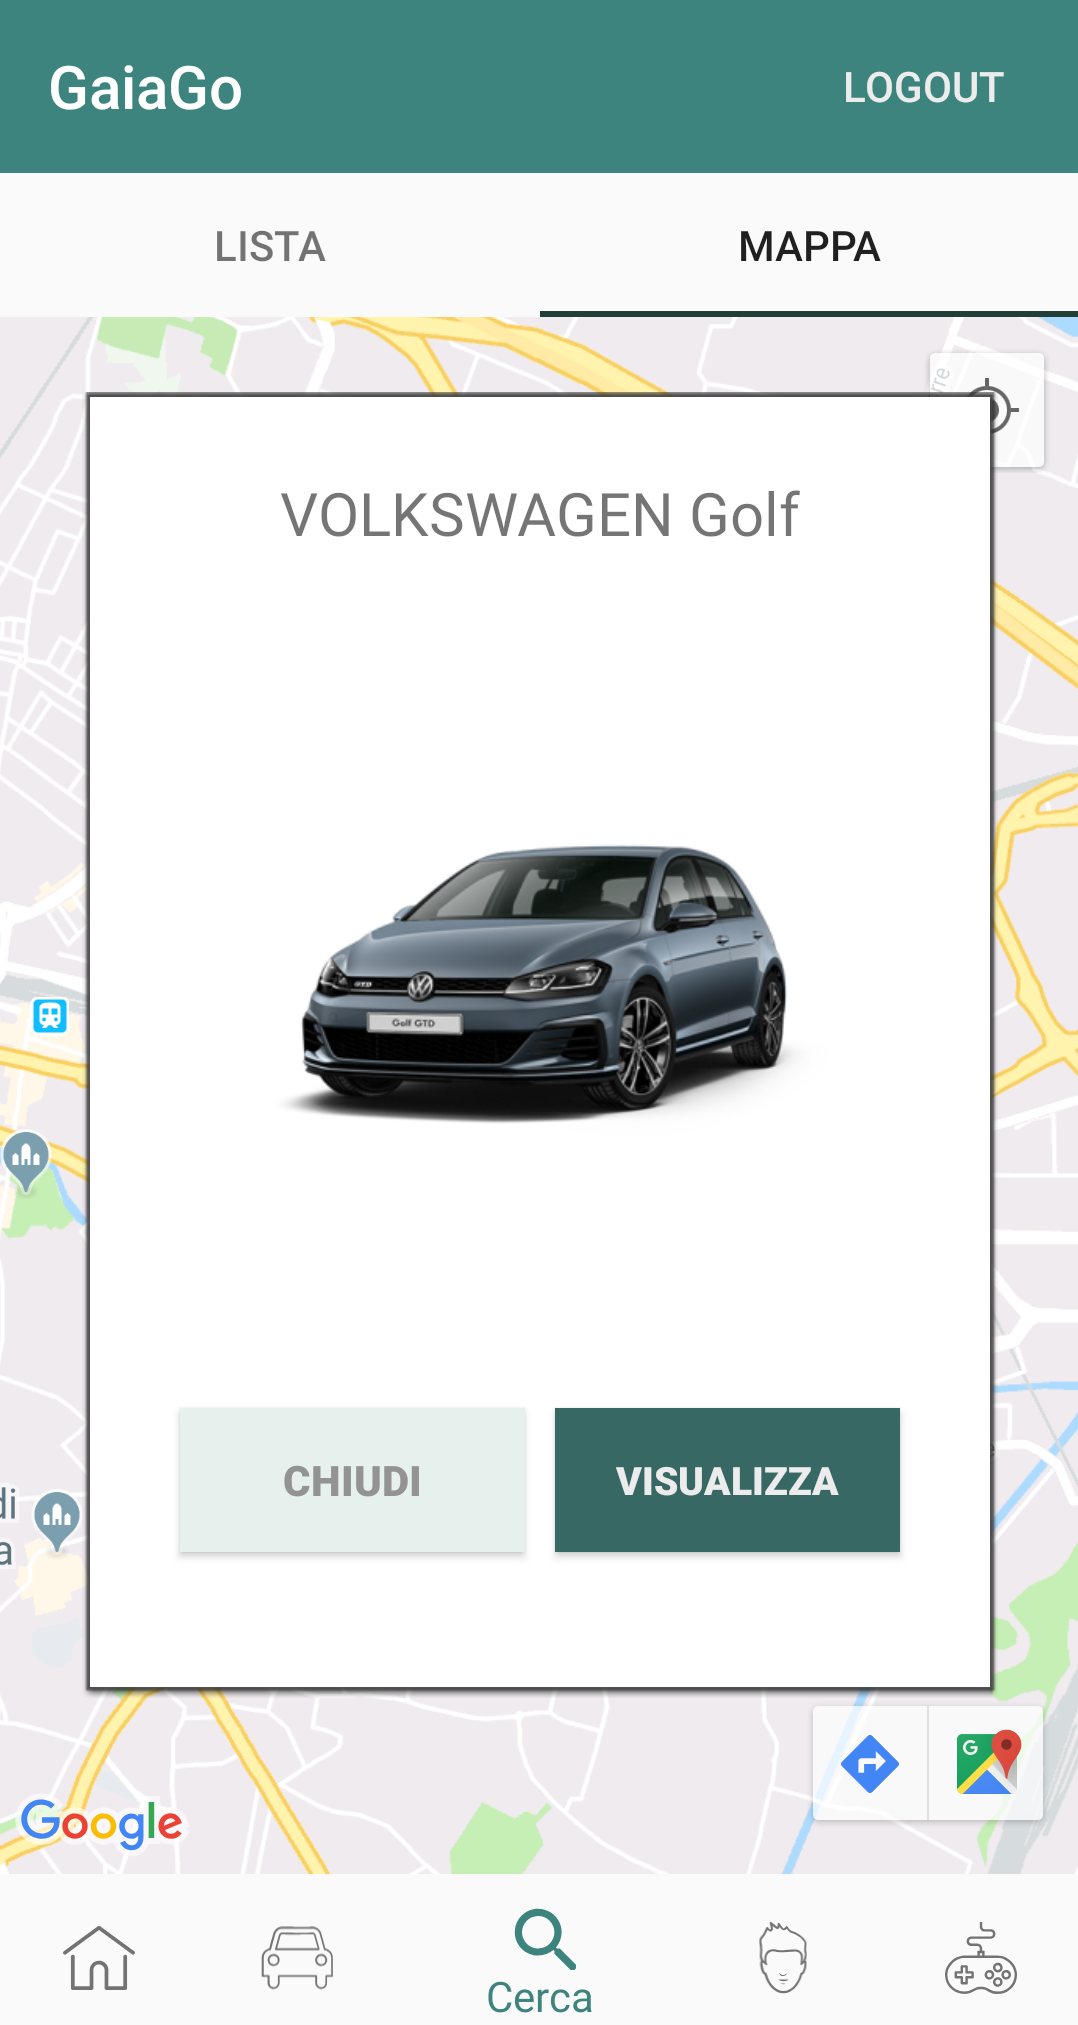
\includegraphics[width=0.5\textwidth]{res/images/mapparicerca2.png}\\
		\caption{Selezione maker di ricerca}
		\label{mappa2}
	\end{figure}
\end{itemize}
  
\pagebreak

Per scegliere quale auto prenotare si preme in qualsiasi punto all'interno del riquadro dell'auto desiderata e si viene portati alla seguente schermata:
  \begin{figure}[H] 
	\centering 
	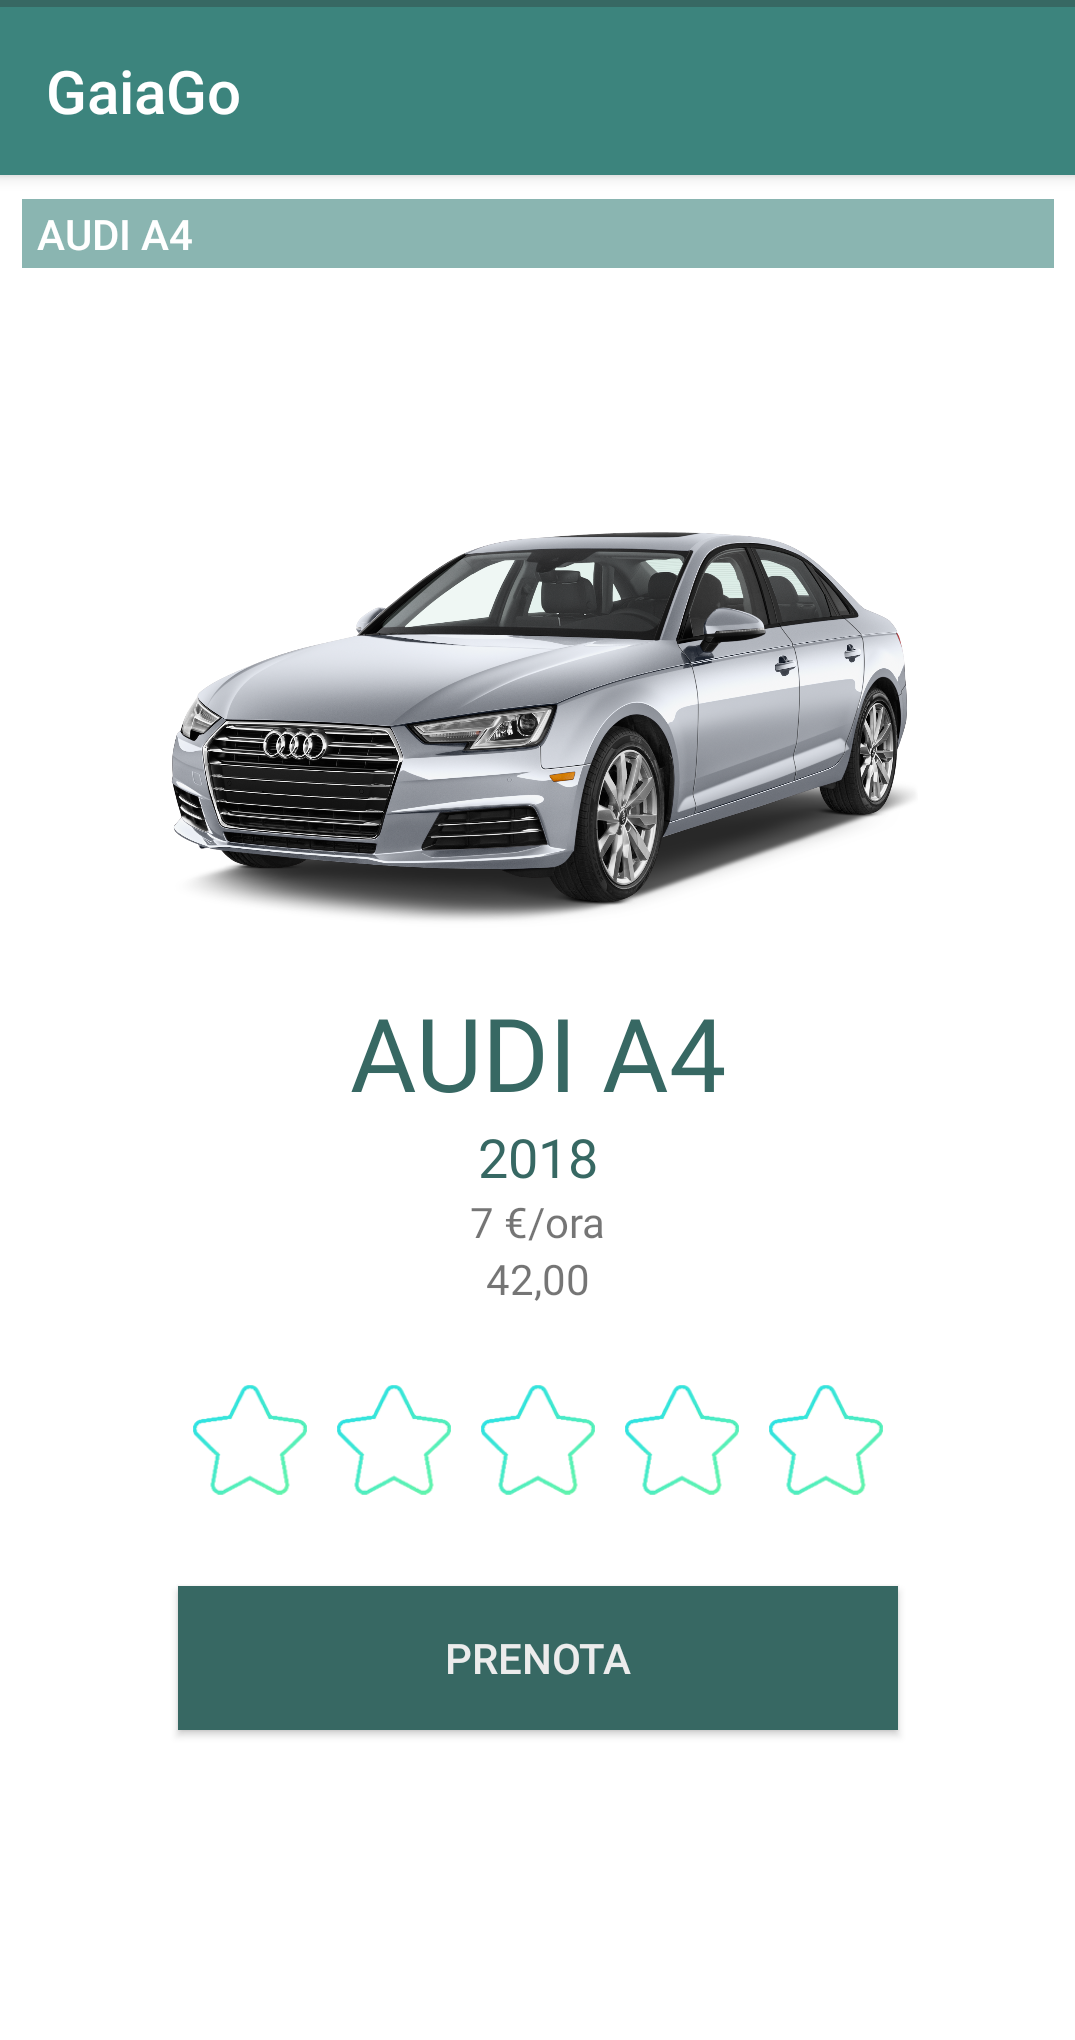
\includegraphics[width=0.5\textwidth]{res/images/prenotazione1.png}\\
	\caption{Auto scelta}
	\label{scelta}
\end{figure}
Qui sono riportati la foto, la marca, il modello, l'anno di immatricolazione, il costo orario totale calcolato in base alla fascia oraria in cui è stato ricercato e il rating\glosp ricevuto dagli utenti che ne hanno fatto utilizzo. Per richiedere la prenotazione si preme sul pulsante verde "PRENOTA".
\pagebreak

\subsection{Gestione prenotazioni}
\label{gestione}
Nell'attività di gestione delle prenotazioni l'utente può vedere i veicoli che ha prenotato e/o i suoi veicoli che sono stati prenotati da altri, per accedervi basta premere nella barra di navigazione il pulsante con una casa stilizzata, una volta premuto ci si sposta sulla sezione con la scritta "Prenotazioni".
  \begin{figure}[H] 
	\centering 
	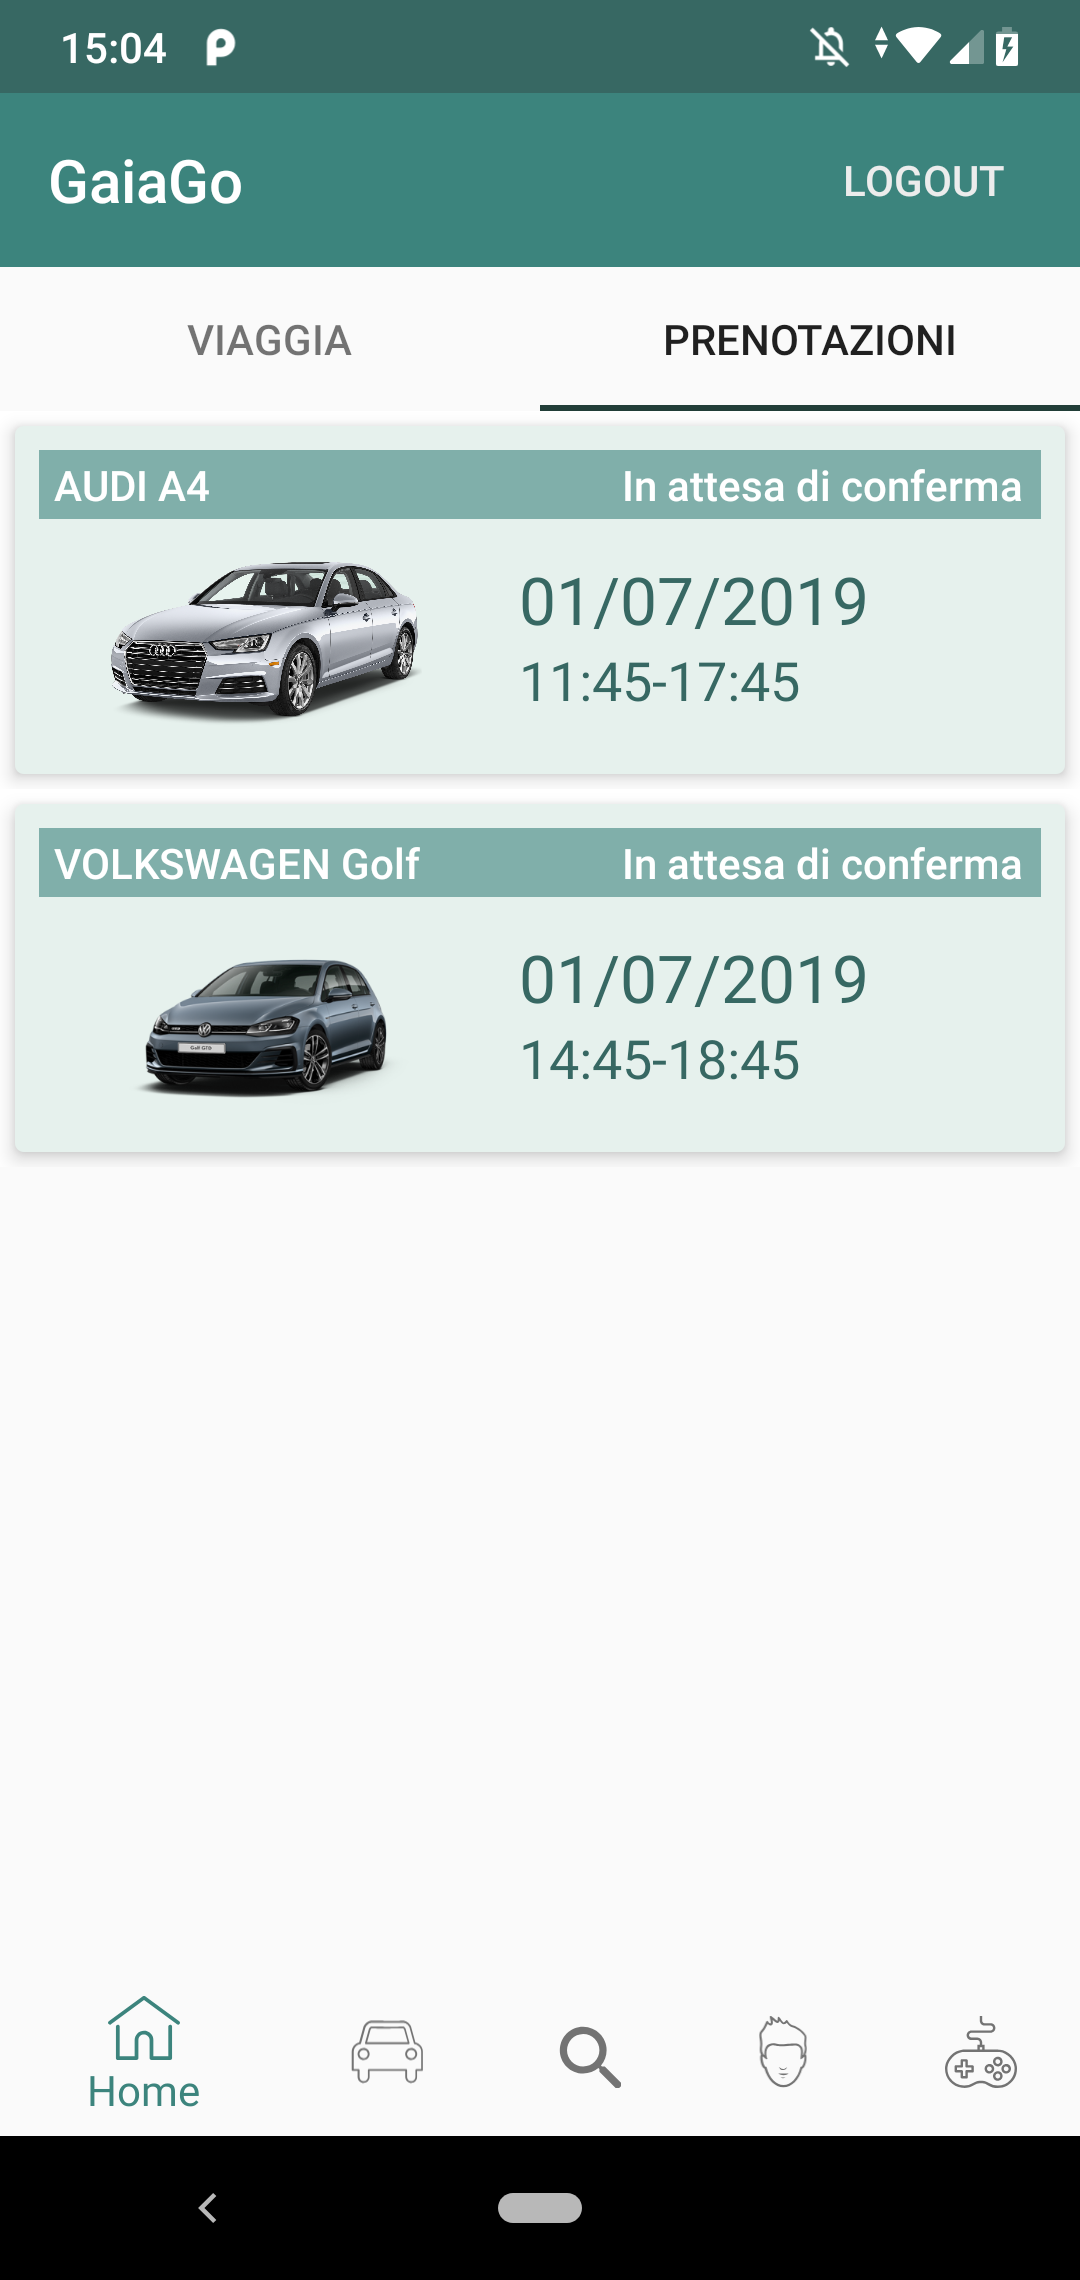
\includegraphics[width=0.5\textwidth]{res/images/prenotazione_effettuata.png}\\
	\caption{Lista auto prenotate}
	\label{prenotate}
\end{figure}
\pagebreak

Ora suddividiamo le prenotazioni in base al tipo:
\begin{itemize}
	\item \textbf{utente}: dopo aver prenotato un veicolo tramite la ricerca questo sarà presente nella schermata sopracitata, se si va a premere sul riquadro corrispondente si apre una nuova sotto-attività nella quale è possibile vedere il dettaglio della prenotazione, comprendente gli orari, giorno, indirizzo e stato, il quale viene modificato se il proprietario accetta/rifiuta. È inoltre possibile annullare la prenotazione tramite il tasto "ANNULLA";
	  \begin{figure}[H] 
		\centering 
		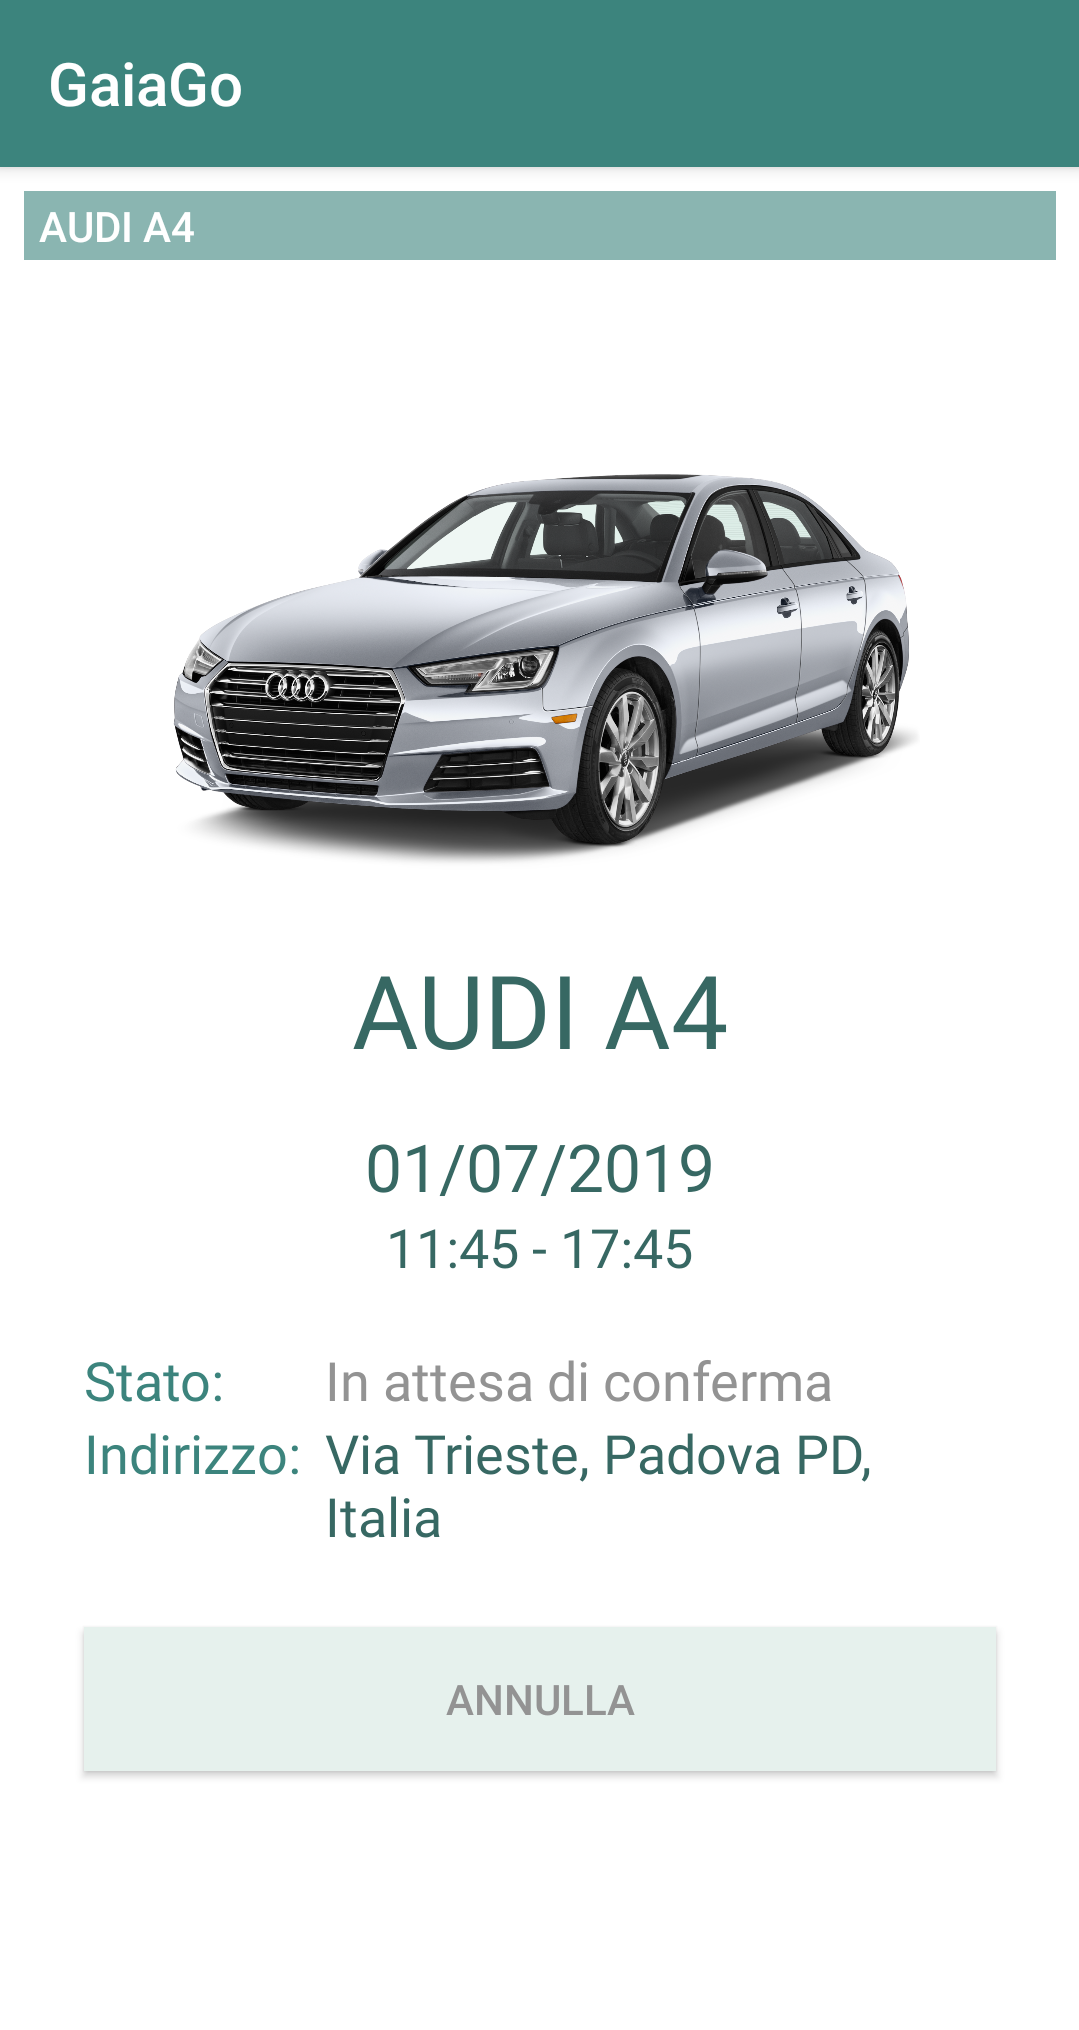
\includegraphics[width=0.5\textwidth]{res/images/annulla_usufruente.png}\\
		\caption{Annulla prenotazione lato usufruente}
		\label{annulla}
	\end{figure}
\pagebreak
	Dopo che il proprietario del veicolo ha confermato la prenotazione, verrà mostrata la seguente schermata:
	\begin{figure}[H] 
		\centering 
		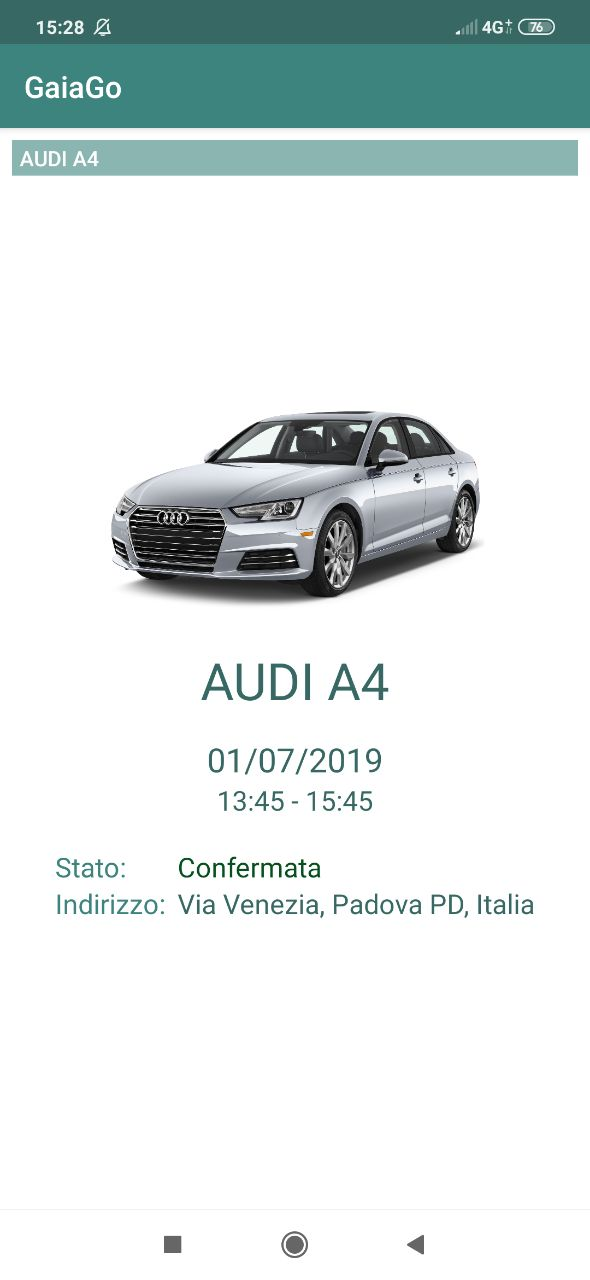
\includegraphics[width=0.5\textwidth]{res/images/conferma_usufruente.png}\\
		\caption{Prenotazione confermata lato usufruente}
		\label{conferma usufruente}
	\end{figure}
	Non appena si effettua la consegna del mezzo e delle chiavi con conseguente conferma del proprietario tramite relativo pulsante, l'usufruente si troverà il cambio di stato da "Confermata" a "In corso".
	\\ \\ \\
	Dopo aver finito di utilizzare l'auto e dopo aver riconsegnato il veicolo e le chiavi al proprietario che a sua volta conclude la prenotazione tramite apposito pulsante, all'usufruente verrà mostrata la seguente schermata:
	\begin{figure}[H] 
		\centering 
		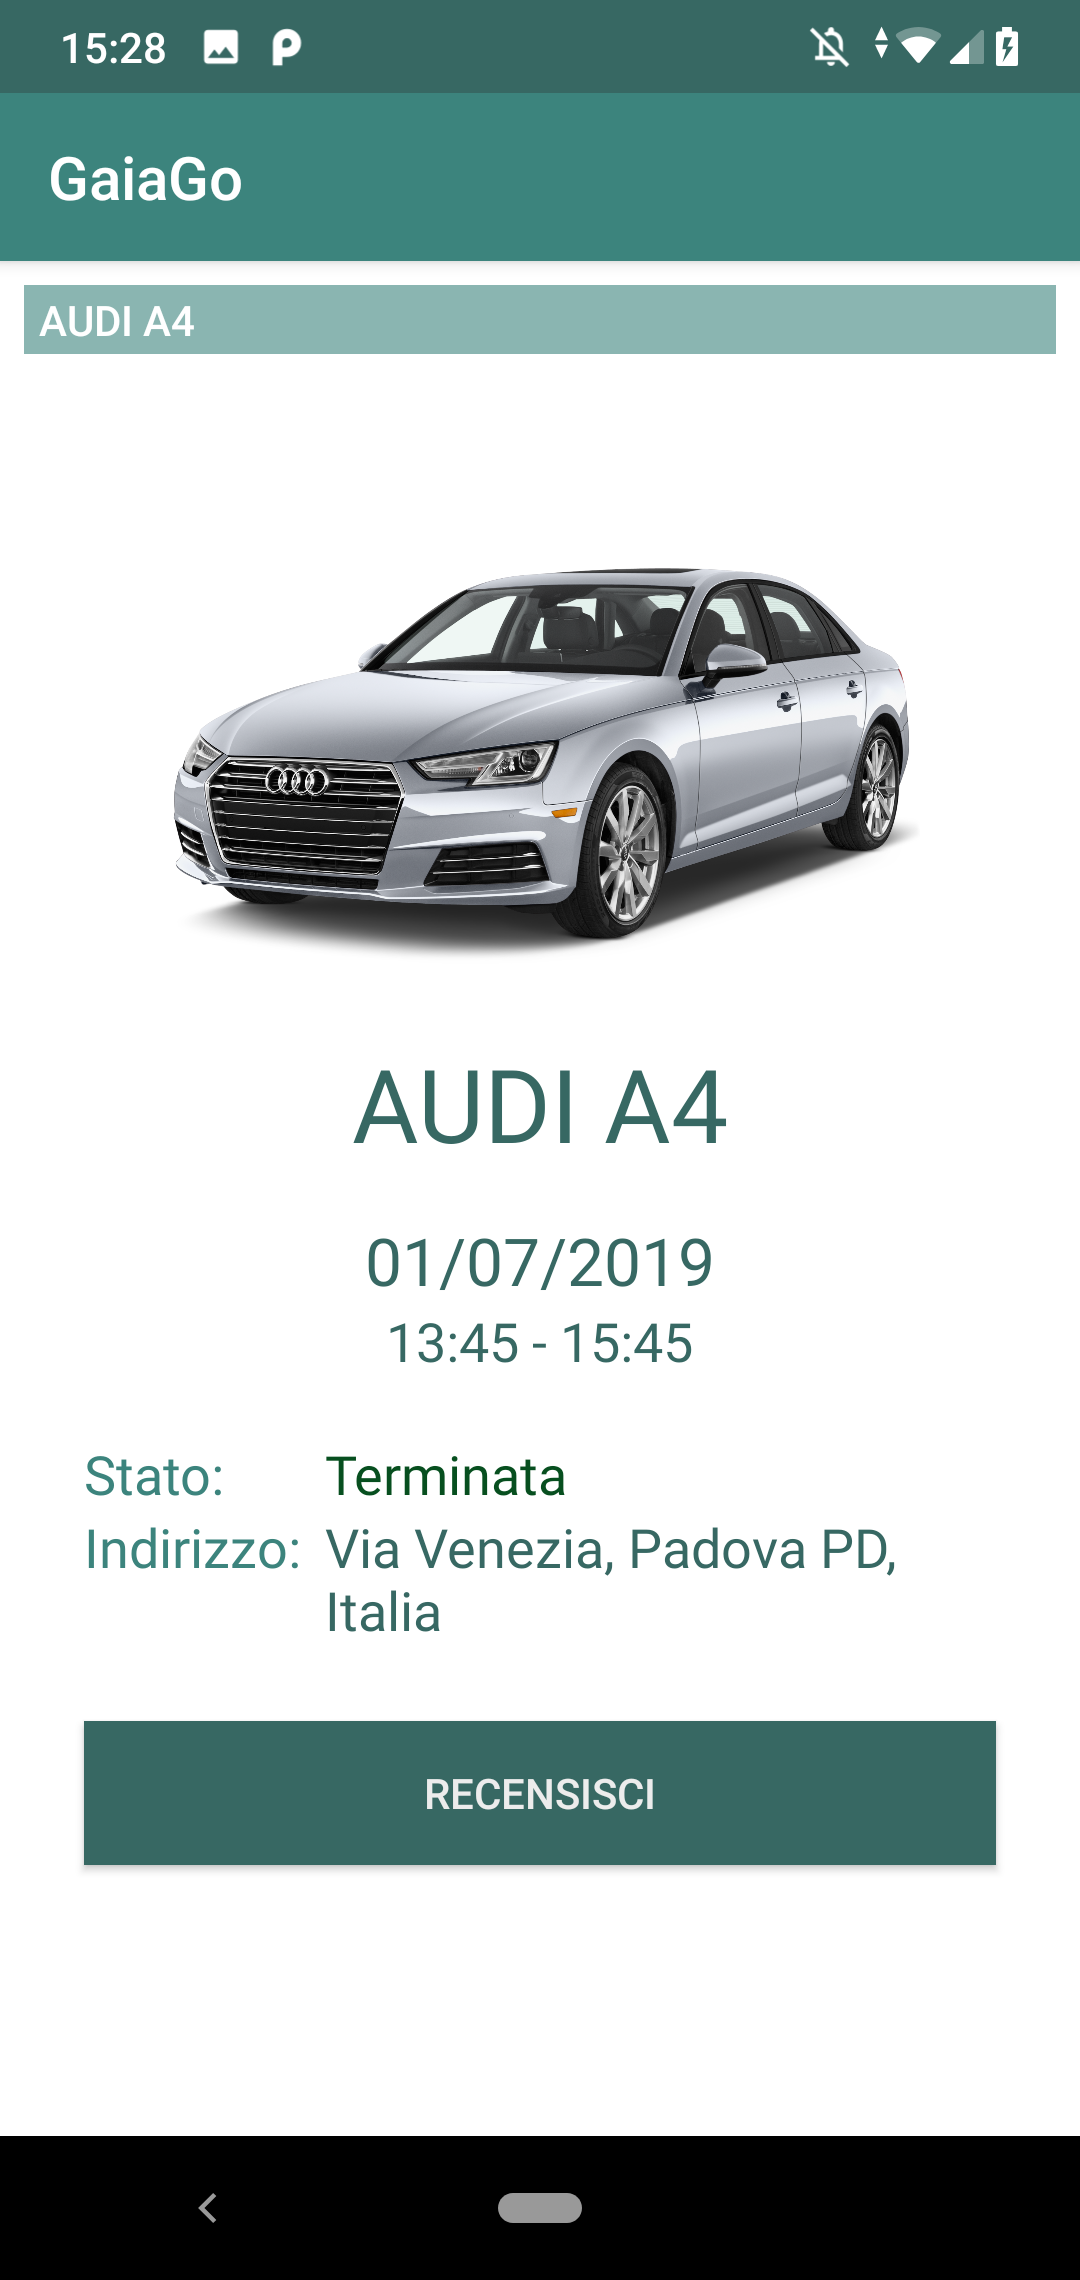
\includegraphics[width=0.5\textwidth]{res/images/recensisci.png}\\
		\caption{Recensione lato usufruente}
		\label{recensisci}
	\end{figure}
	Premendo il pulsante "RECENSISCI" l'usufruente potrà recensire, attraverso un pop-up tramite la valutazione da 1 a 5 stelle, il veicolo e il proprietario.\\
	Infine, premendo il pulsante "CONFERMA" per confermare la recensione appena inserita, verrà mostrata la schermata in cui può archiviare la prenotazione appena conclusa. 

\pagebreak
	\item \textbf{proprietario}: dopo aver messo a disposizione un veicolo perché venga prenotato, ed un utente ne richiede la prenotazione, nella schermata contenente tutte le prenotazioni è possibile cliccare sulla propria auto e si viene condotti alla schermata per la conferma o rifiuto della prenotazione, contiene inoltre tutti i dati riguardanti gli orari e il giorno richiesti.
	  \begin{figure}[H] 
		\centering 
		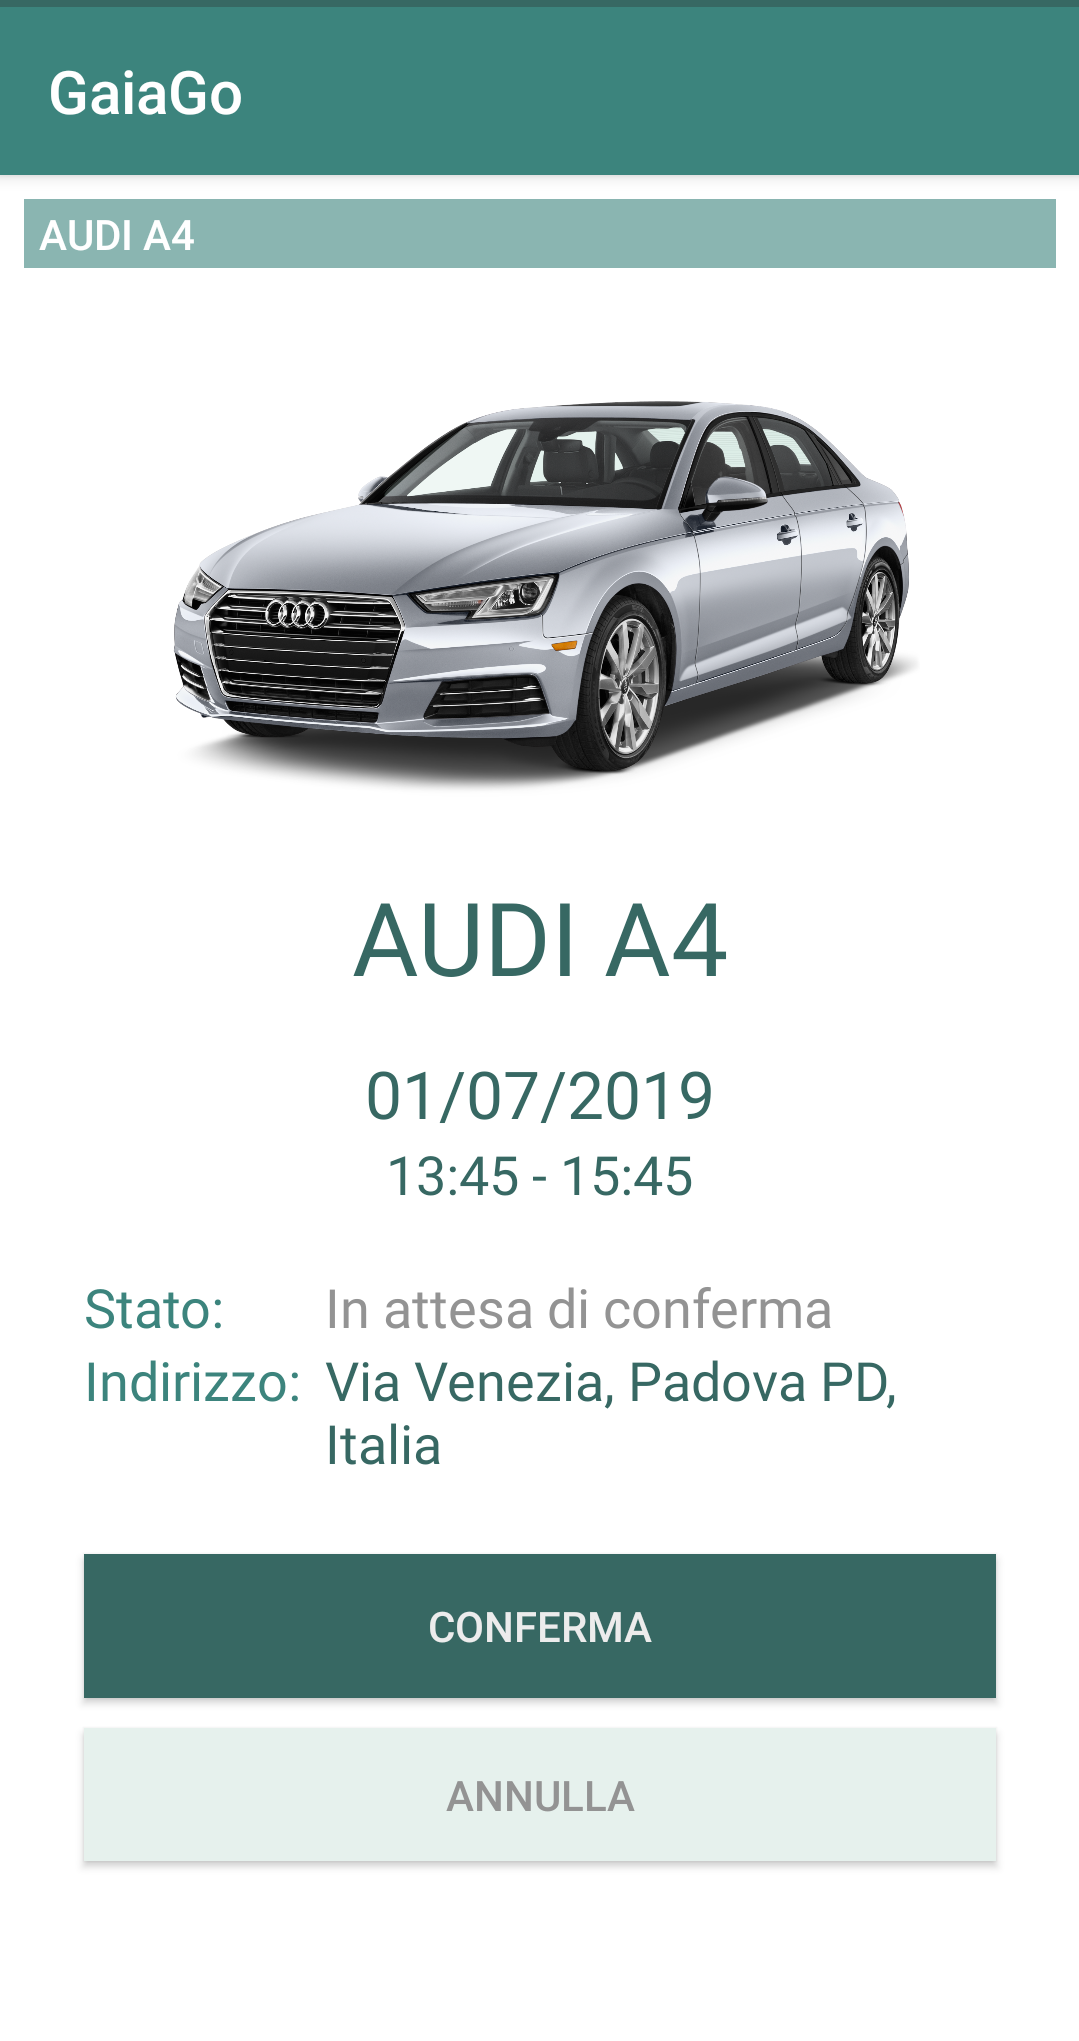
\includegraphics[width=0.5\textwidth]{res/images/conferma_proprietario.png}\\
		\caption{Conferma prenotazione lato proprietario}
		\label{conferma prenotazione}
	\end{figure}
	\pagebreak
	Successivamente viene cambiato lo stato della prenotazione in "Confermata" e mostrato la seguente schermata:
	\begin{figure}[H] 
		\centering 
		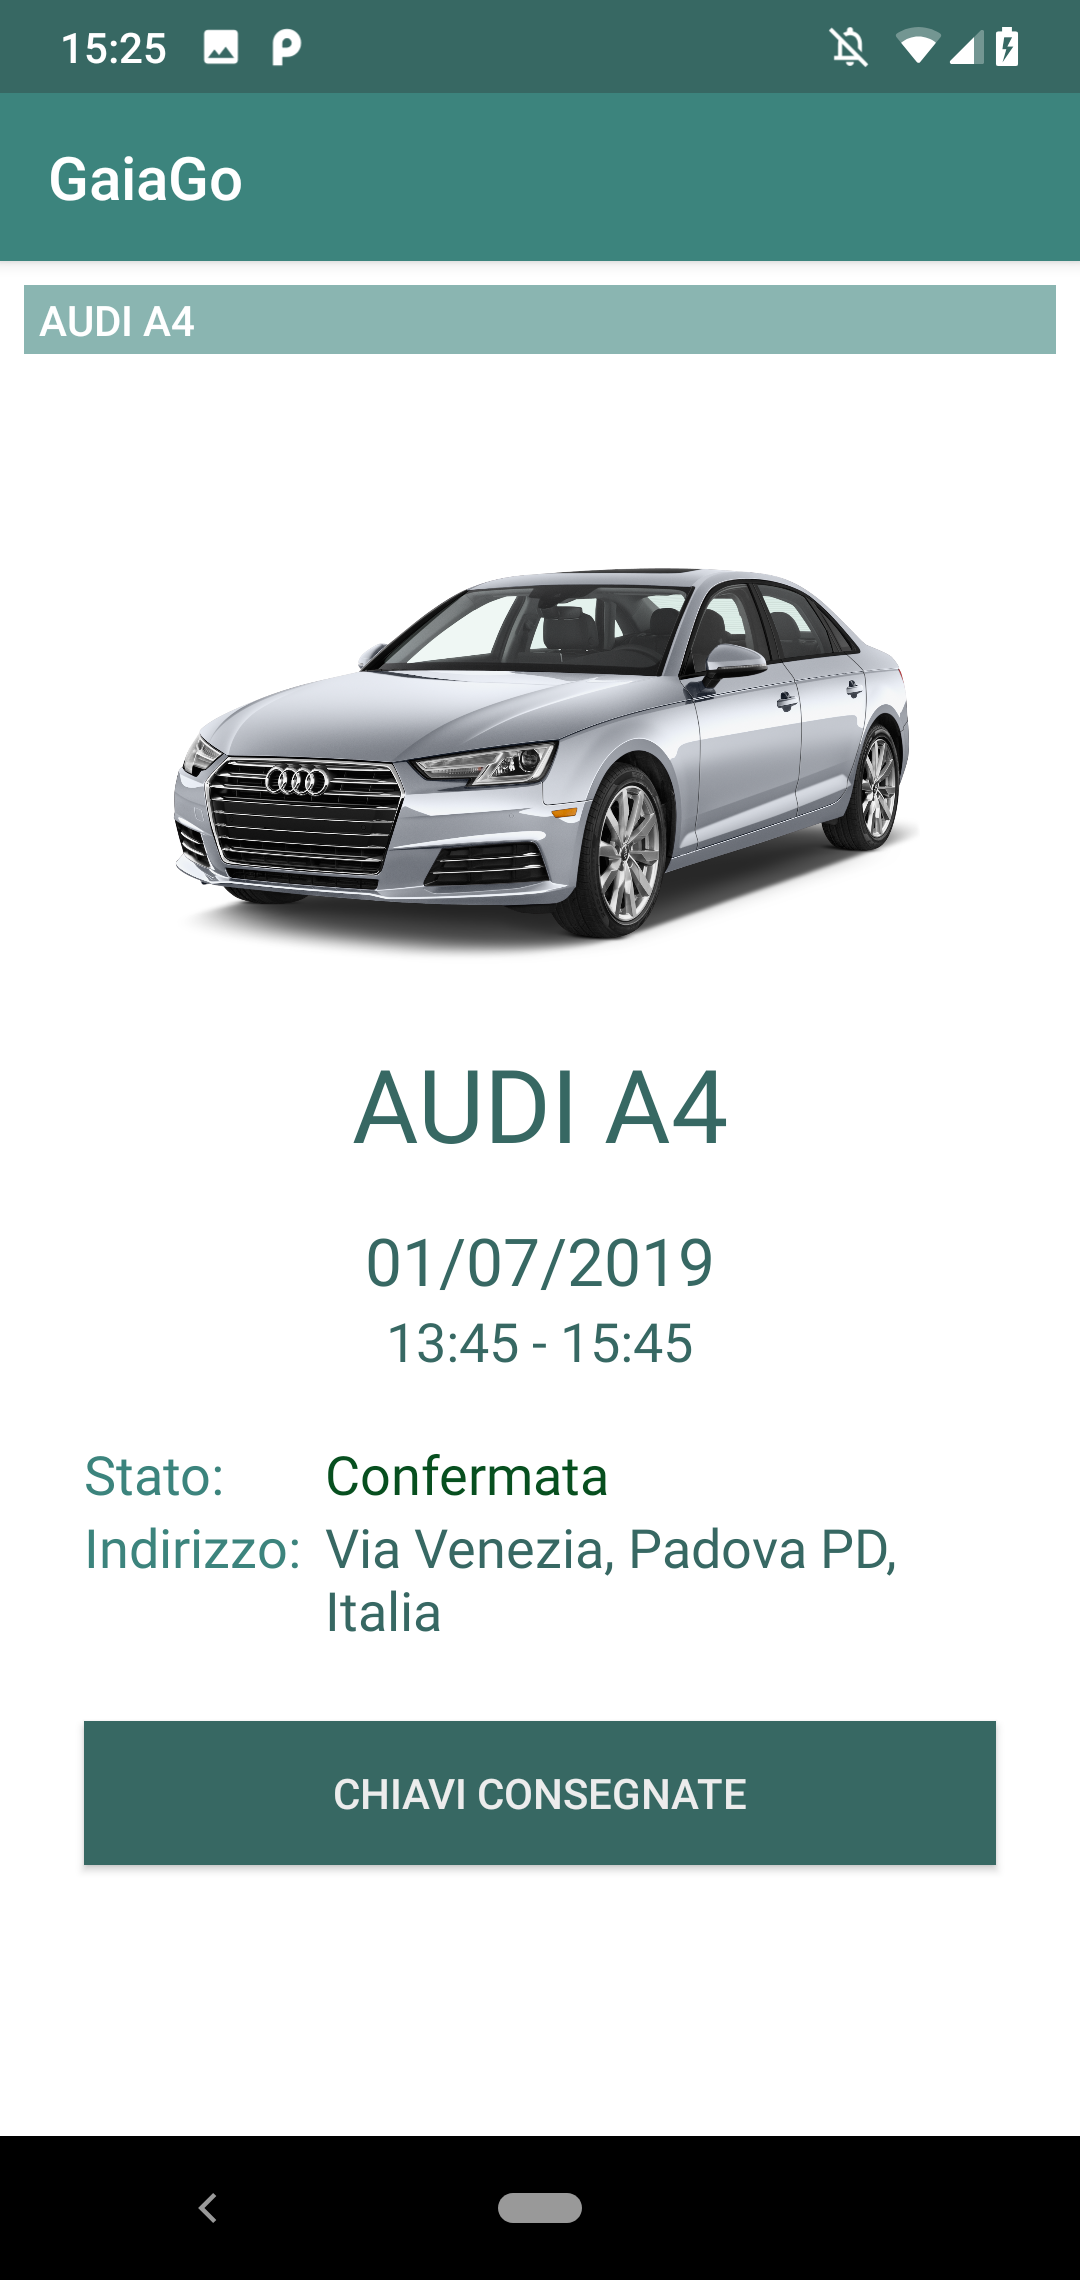
\includegraphics[width=0.5\textwidth]{res/images/chiavi_proprietario.png}\\
		\caption{Richiesta di prenotazione}
		\label{chiavi}
	\end{figure}
\pagebreak
	Dopo che il proprietario abbia confermato di aver consegnato le chiavi all'usufruente e aver premuto il pulsante corrispondente, verrà mostrata la seguente schermata:
	\begin{figure}[H] 
		\centering 
		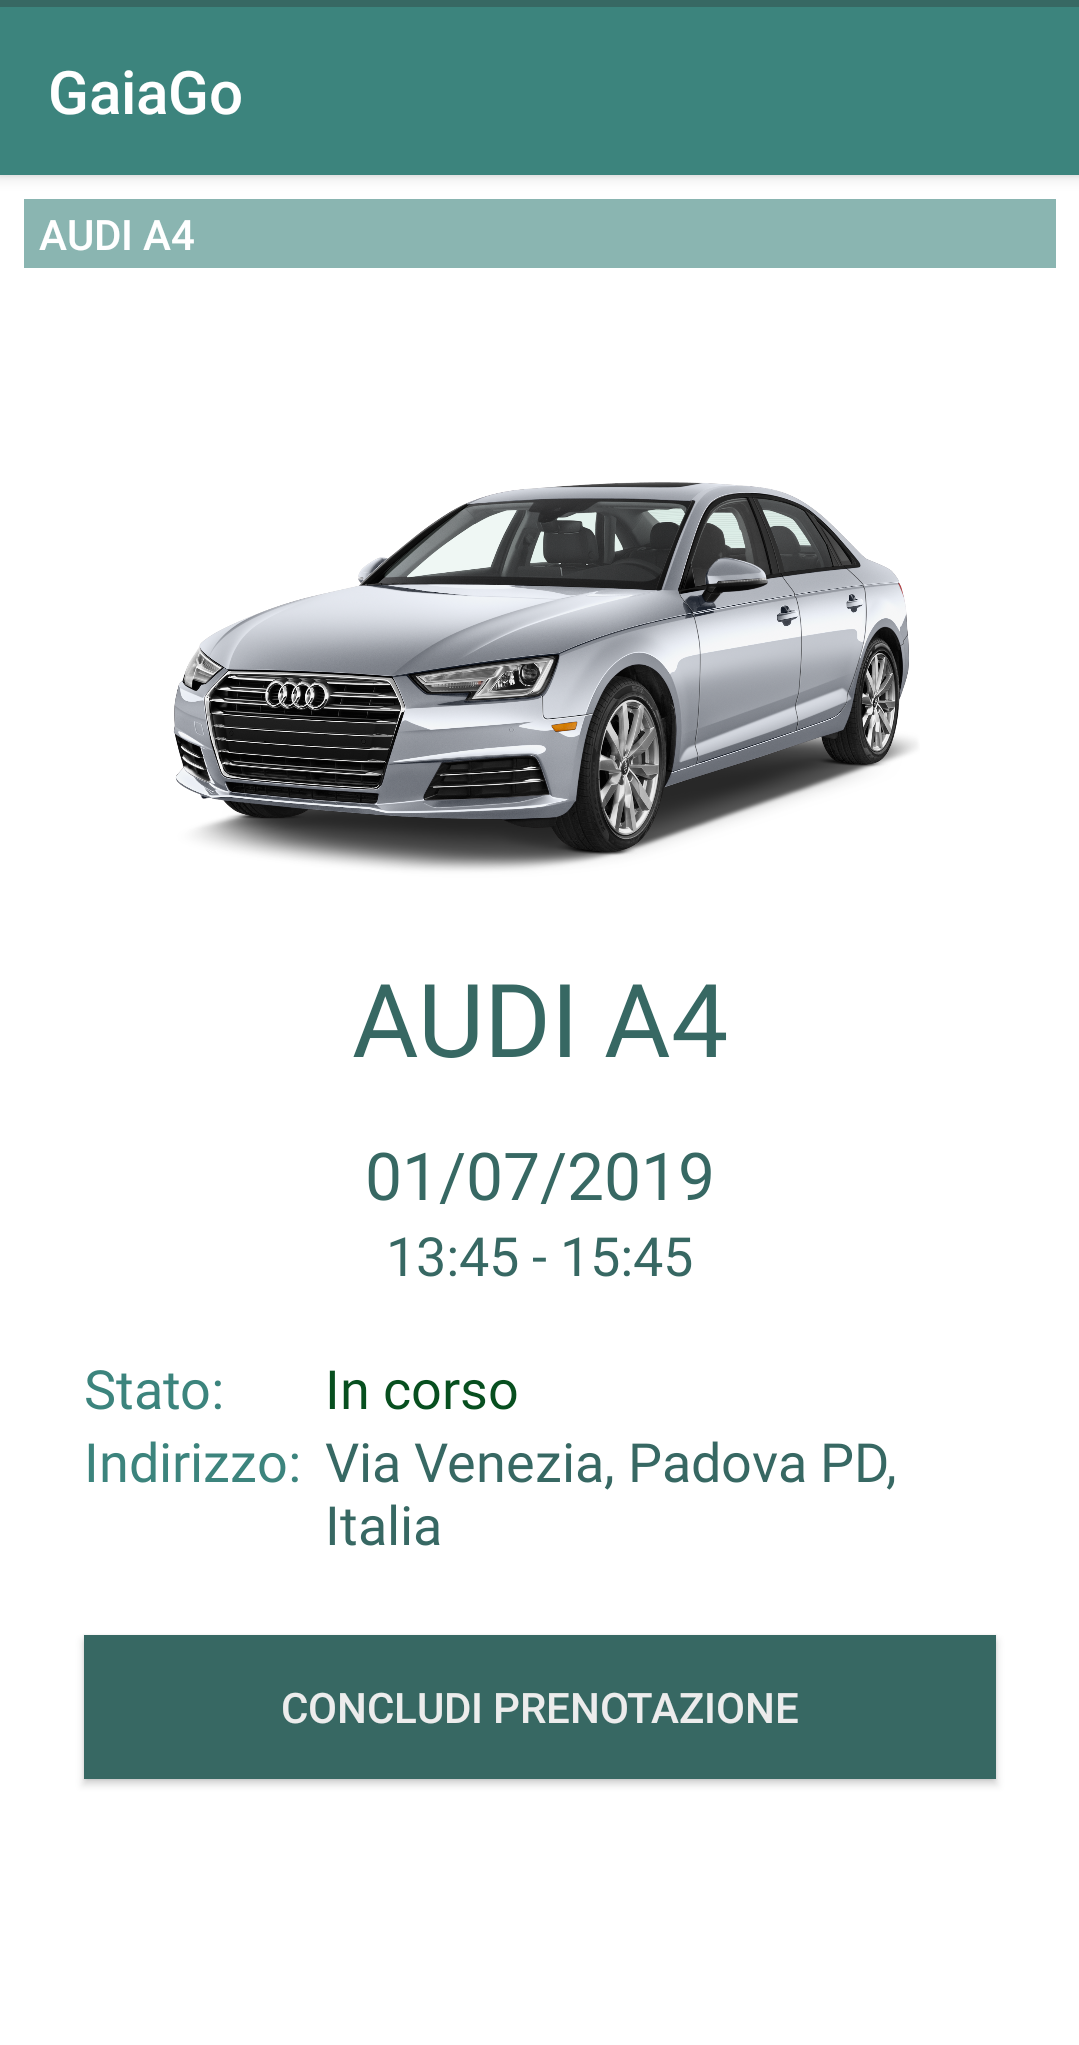
\includegraphics[width=0.5\textwidth]{res/images/concludi_proprietario.png}\\
		\caption{Chiusura prenotazione lato proprietario}
		\label{chiusura}
	\end{figure}
\pagebreak
	Dopo aver ricevuto dall'usufruente le chiavi e il veicolo riconsegnati, il proprietario potrà chiudere la prenotazione e dopo aver premuto il tasto "CONCLUDI PRENOTAZIONE" verrà mostrata la seguente schermata:
	\begin{figure}[H] 
		\centering 
		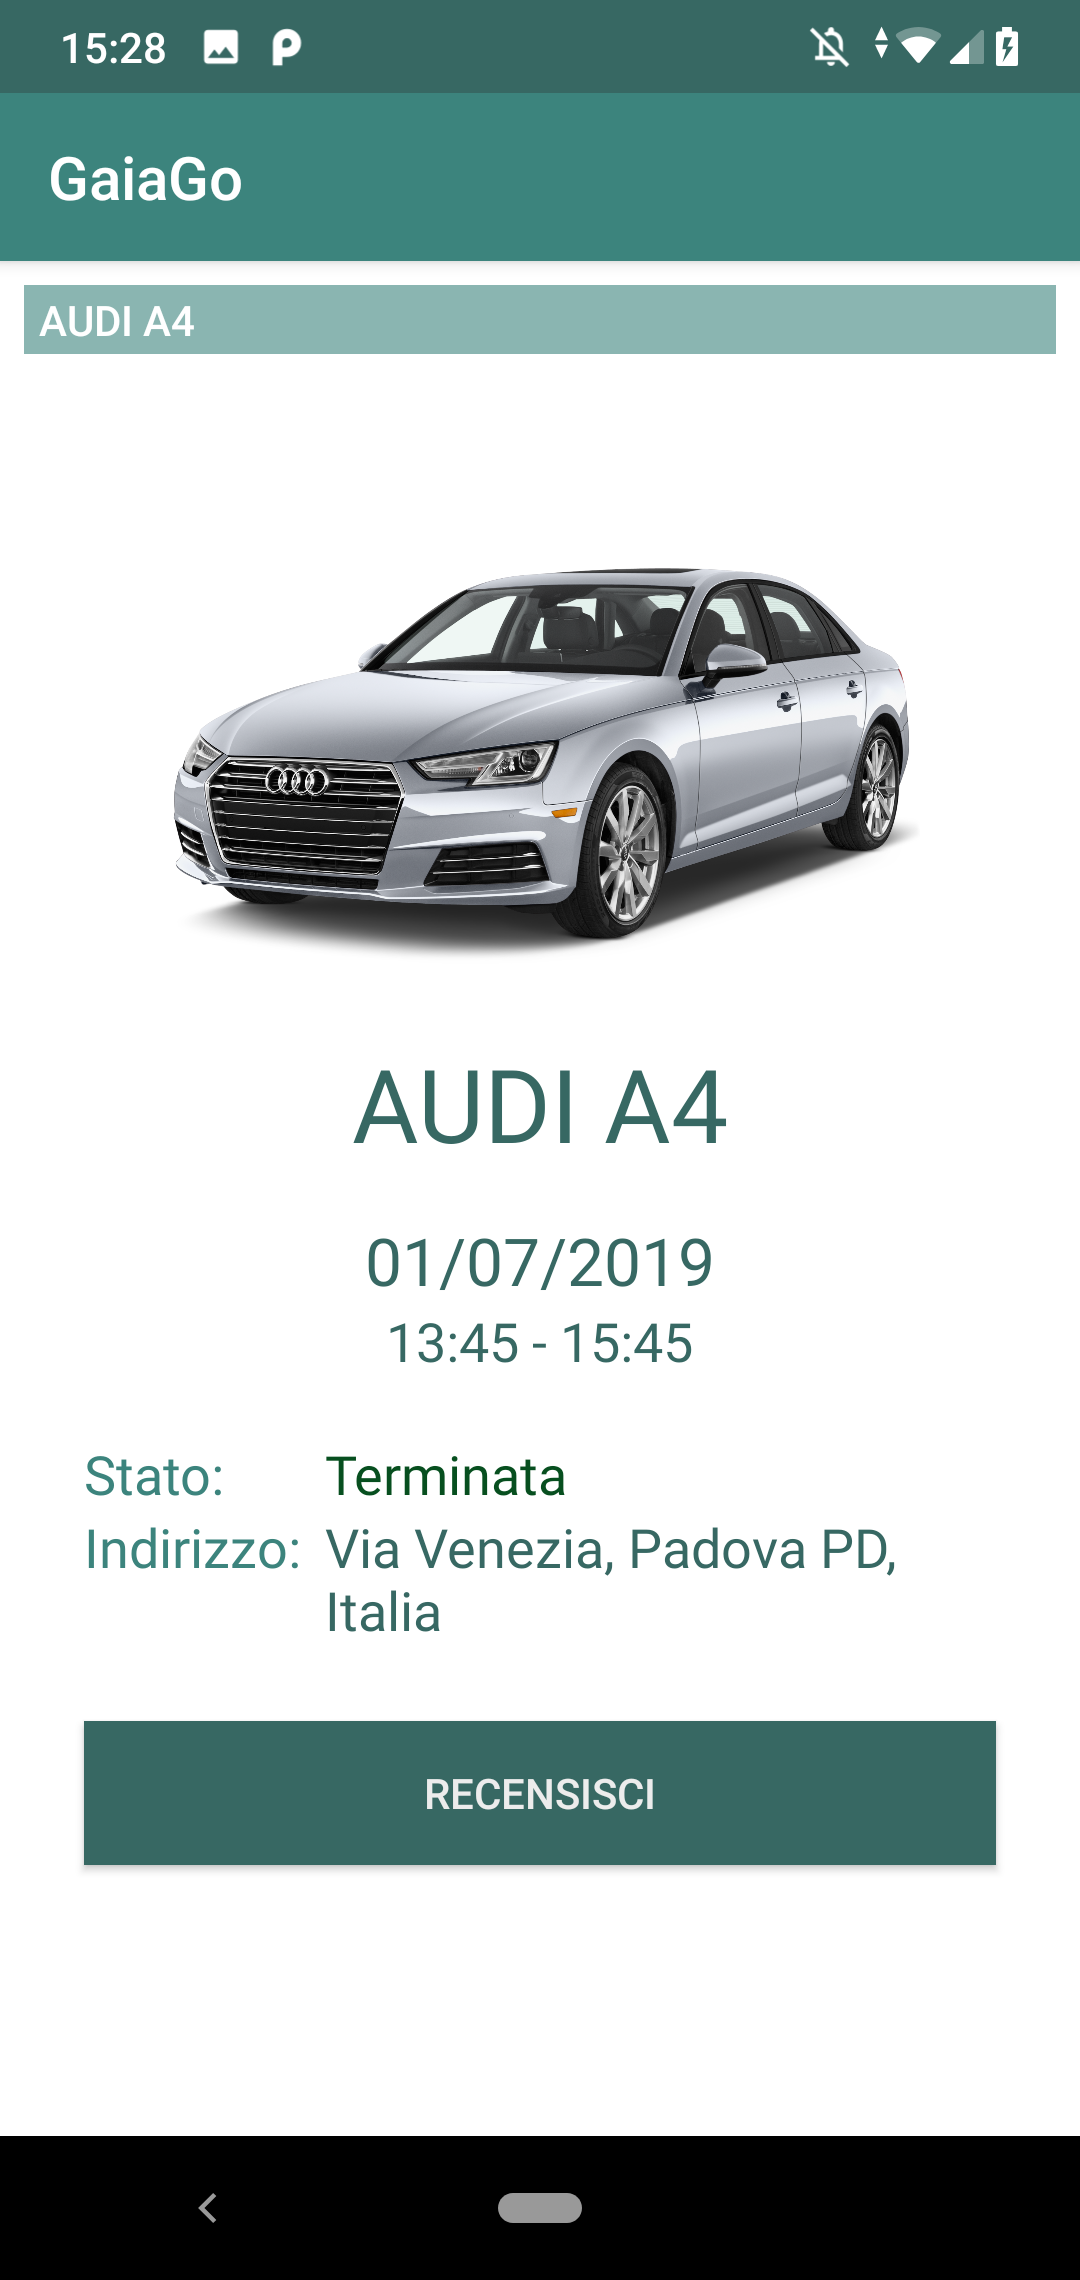
\includegraphics[width=0.5\textwidth]{res/images/recensisci.png}\\
		\caption{Recensione lato proprietario}
		\label{recensione}
	\end{figure}
\pagebreak
	Infine, premuto il tasto "RECENSISCI" all'utente verrà mostrato un pop-up in cui dovrà inserire un numero di stelle da 1 a 5 per valutare l'utente usufruente.
	\begin{figure}[H] 
		\centering 
		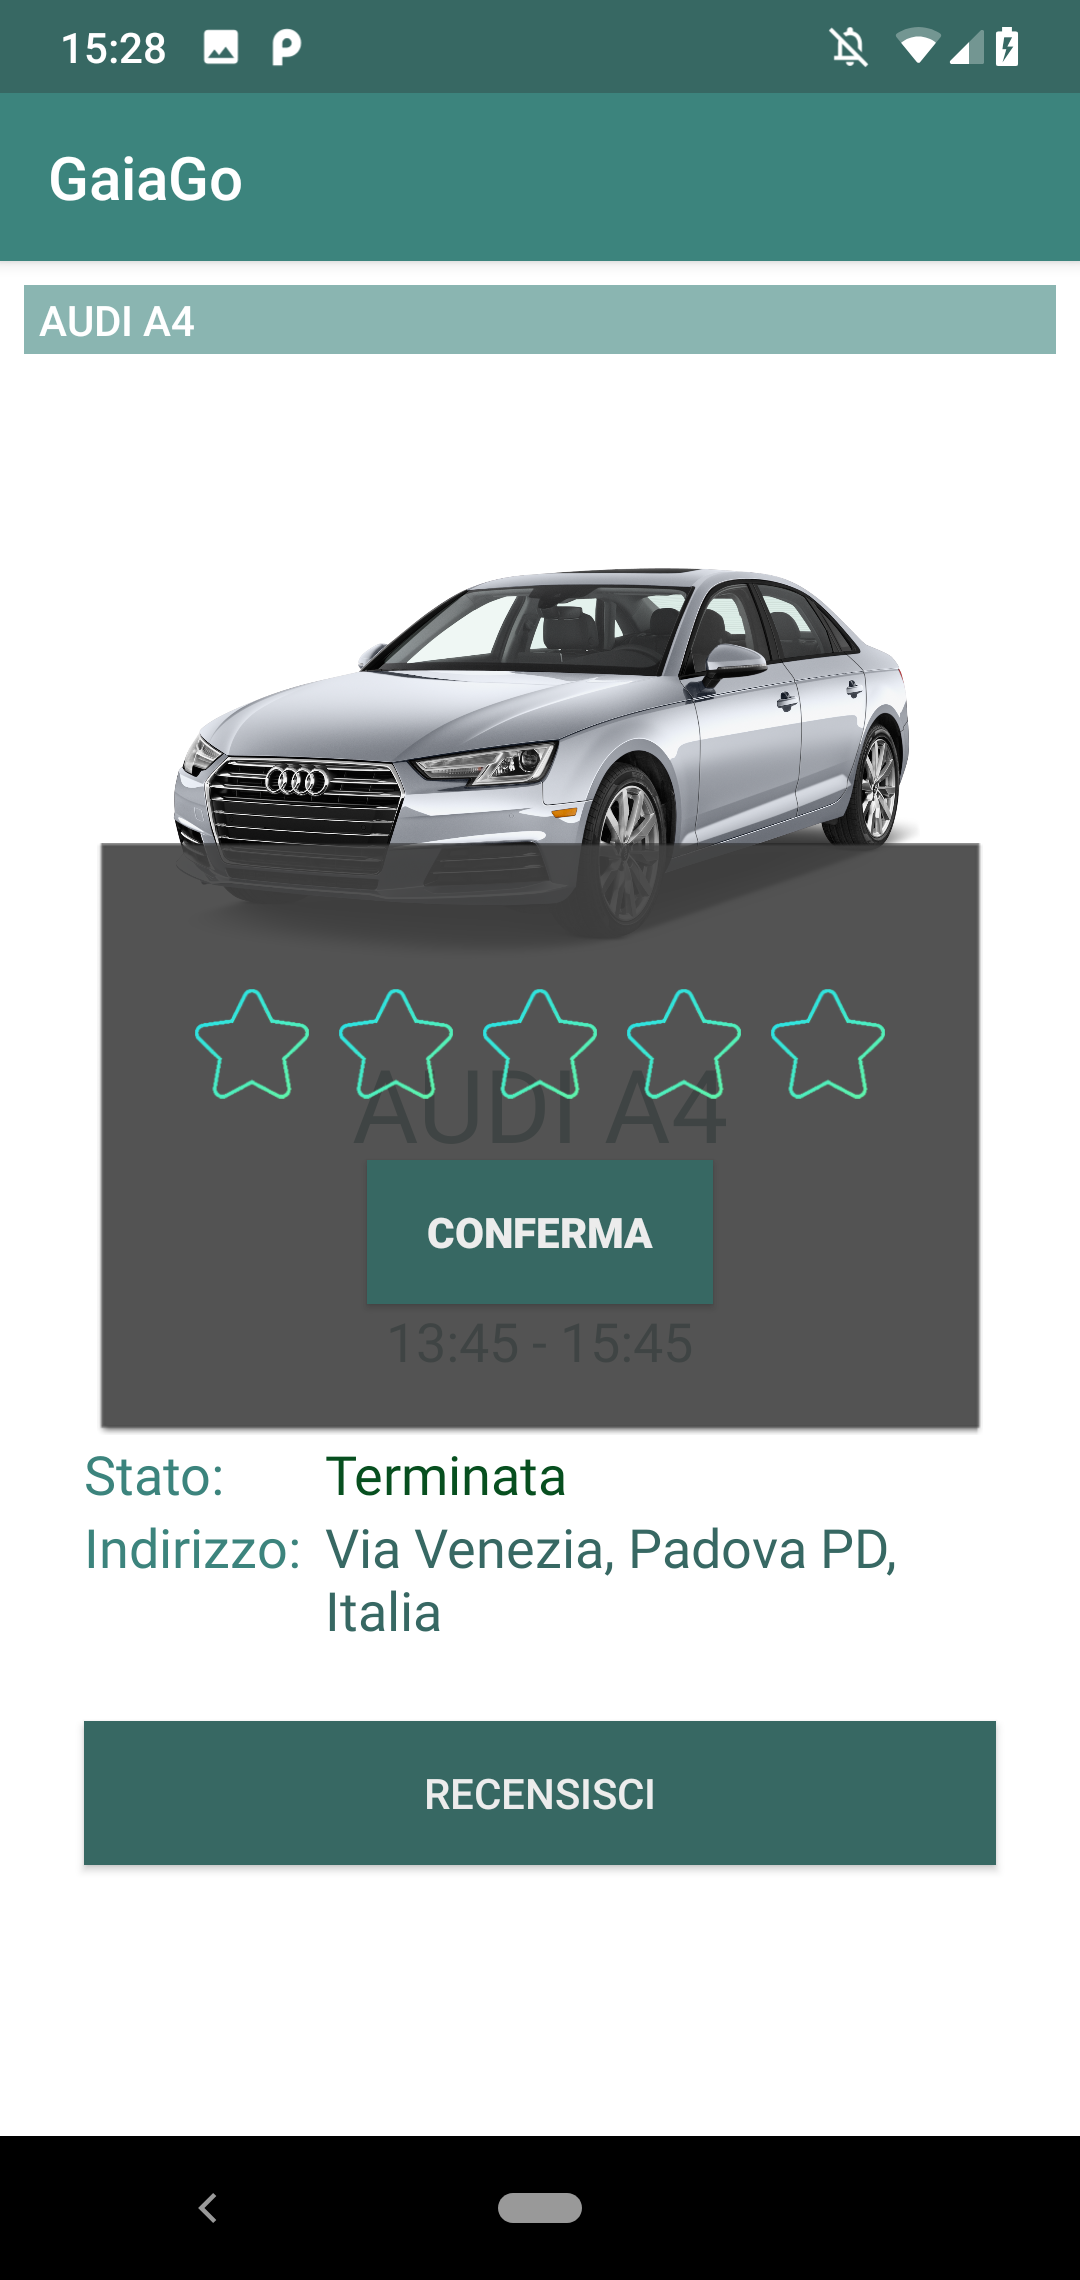
\includegraphics[width=0.5\textwidth]{res/images/recensione.png}\\
		\caption{Recensione lato proprietario}
		\label{recensione2}
	\end{figure}
\pagebreak
	Per ultima cosa, dopo aver premuto il pulsante "CONFERMA" per confermare la recensione appena inserita, verrà mostrata la seguente schermata in cui il proprietario potrà archiviare la prenotazione. Archiviandola verrà poi portato alla \textit{Home} dell'applicazione.
	\begin{figure}[H] 
		\centering 
		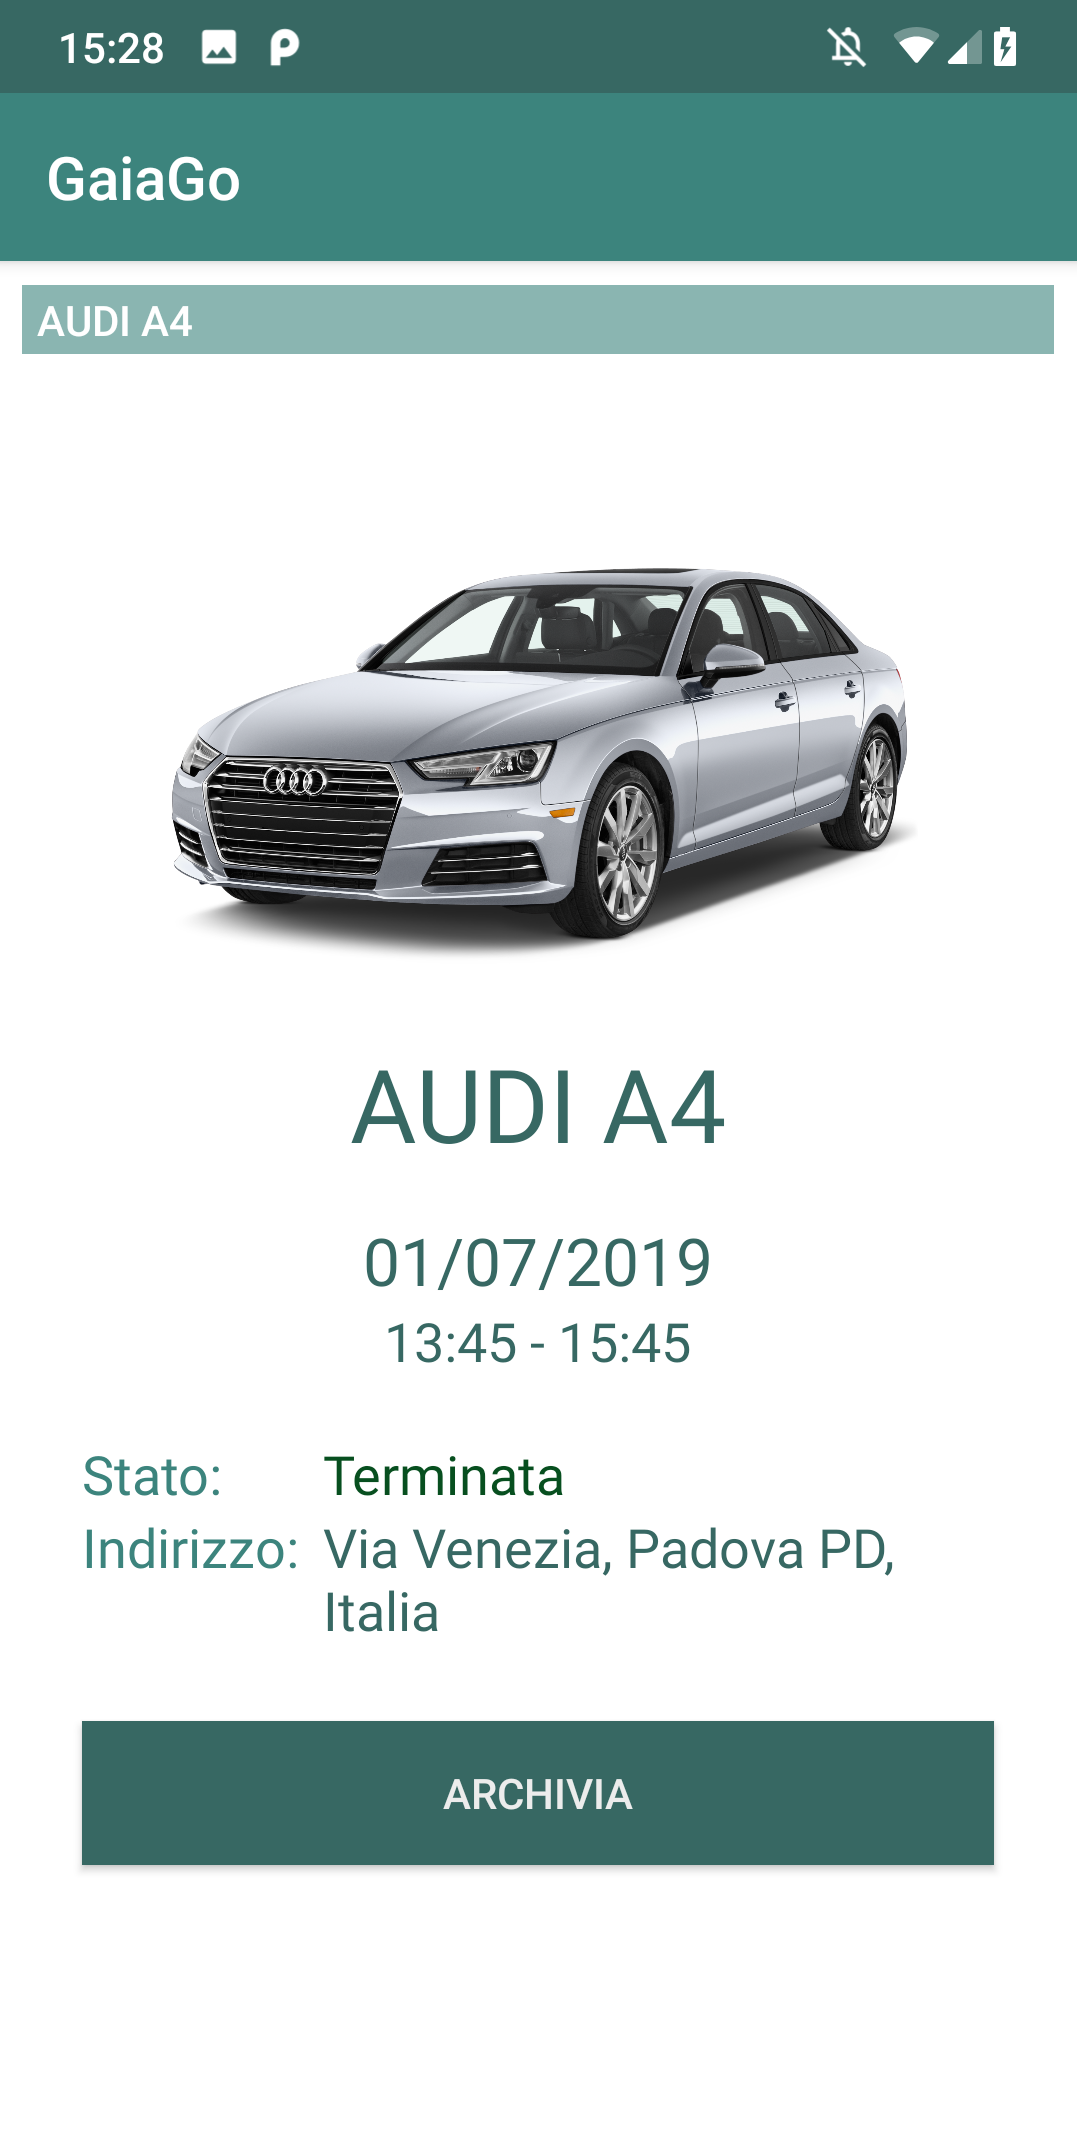
\includegraphics[width=0.5\textwidth]{res/images/archivia_prenotazione.png}\\
		\caption{Recensione lato proprietario}
		\label{archivia}
	\end{figure}
\end{itemize}
\pagebreak

\subsection{Profilo utente}
Questa sezione include tutti i dati dell'utente corrente. Presenta la patente, nome e cognome, numero di cellulare, email, data di nascita e indirizzo di residenza.
 \begin{figure}[H] 
	\centering 
	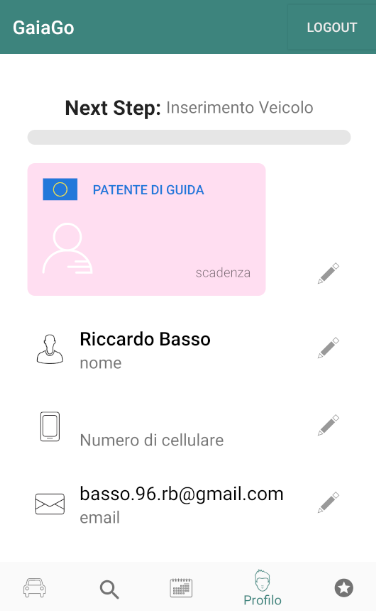
\includegraphics[width=0.5\textwidth]{res/images/profilo_utente.png}\\
	\caption{Profilo utente}
	\label{profilo}
\end{figure}
\pagebreak

Ogni campo risulta modificabile, di seguito è mostrato passo passo la procedura da seguire per ognuno:
\begin{itemize}
	\item \textbf{patente di guida}: cliccando sull'icona a forma di penna, a destra dell'immagine della patente, si passa alla fase di inserimento e modifica;
	 \begin{figure}[H] 
		\centering 
		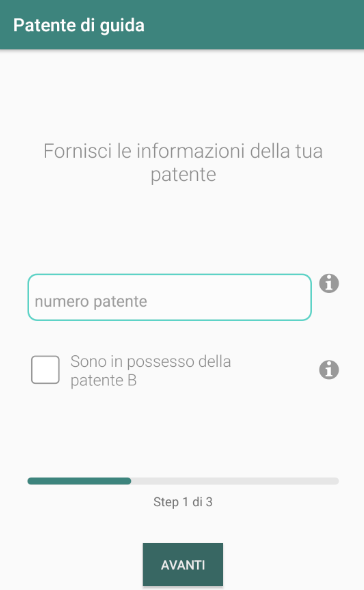
\includegraphics[width=0.5\textwidth]{res/images/patente1.png}\\
		\caption{Patente}
		\label{patente}
	\end{figure}
\pagebreak

È necessario compilare il campo numero patente. L'utente può ricevere un aiuto premendo il tasto info posto a destra.
 \begin{figure}[H] 
 	\centering 
 	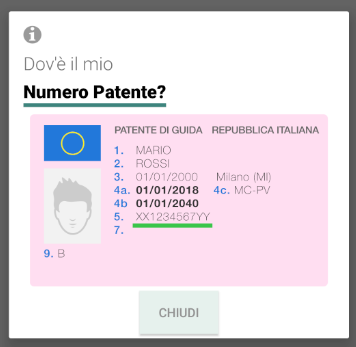
\includegraphics[width=0.5\textwidth]{res/images/patente1_info.png}\\
 	\caption{Info numero patente}
 	\label{patente1}
 \end{figure}
L'errore che si presenta nel caso in cui non venga inserito il numero è il seguente:
 \begin{figure}[H] 
	\centering 
	
\includegraphics[width=0.5\textwidth]{res/images/patente1errore.png}\\
	\caption{Errore numero patente}
	\label{patenteerror}
\end{figure}
\pagebreak

Per inserire la patente è necessario essere in possesso della patente di grado B, un'altra info è disponibile cliccando la relativa icona posta a destra.
\begin{figure}[H] 
	\centering 
	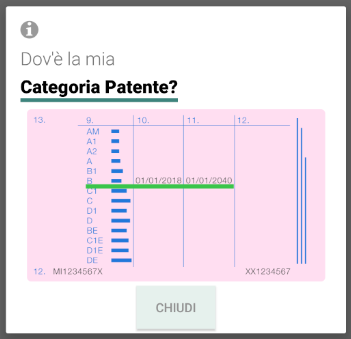
\includegraphics[width=0.5\textwidth]{res/images/patente1_info2.png}\\
	\caption{Info patente B}
	\label{patente2}
\end{figure}
\pagebreak

Al termine dell'inserimento dei dati la schermata si presenta nel modo seguente:
\begin{figure}[H] 
	\centering 
	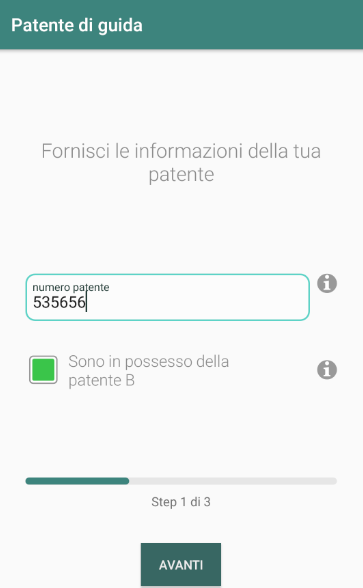
\includegraphics[width=0.5\textwidth]{res/images/patente1_1.png}\\
	\caption{Schermata completata con i relativi campi}
	\label{patente3}
\end{figure}
Per proseguire si prema il pulsante "AVANTI".
\pagebreak

Il prossimo step di inserimento richiede la data di rilascio e la data di scadenza compilabili tramite un calendario come già visto in precedenza.
\begin{figure}[H] 
	\centering 
	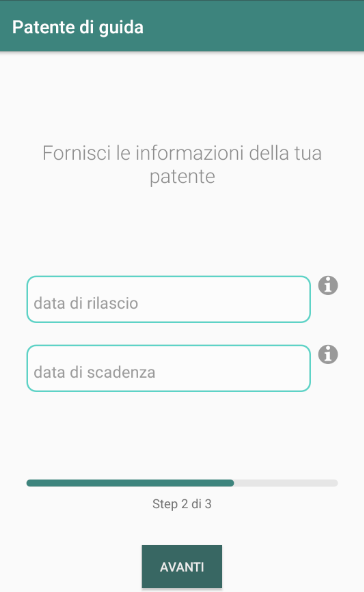
\includegraphics[width=0.5\textwidth]{res/images/patente2.png}\\
	\caption{Seconda schermata patente}
	\label{patente4}
\end{figure}
\pagebreak

Anche in questa sezione sono presenti degli aiuti all'utente per indicare dove cercare le date richieste premendo sul tasto info.
\begin{figure}[H] 
	\centering 
	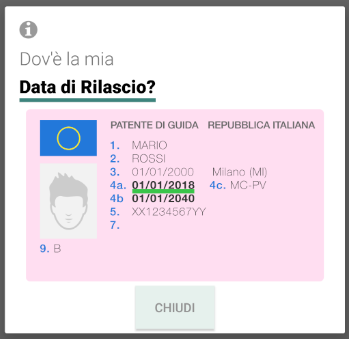
\includegraphics[width=0.5\textwidth]{res/images/patente2_1.png}\\
	\caption{Data di rilascio}
	\label{patente5}
\end{figure}
Errore annesso:
 \begin{figure}[H] 
	\centering 
	
\includegraphics[width=0.5\textwidth]{res/images/patente2errore_rilascio.png}\\
	\caption{Errore data rilascio}
	\label{patenteerror1}
\end{figure}
\begin{figure}[H] 
	\centering 
	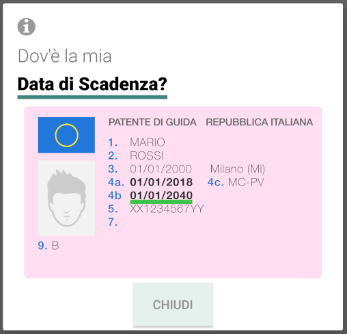
\includegraphics[width=0.5\textwidth]{res/images/patente2_2.png}\\
	\caption{Data di scadenza}
	\label{patente6}
\end{figure}
Errore annesso:
\begin{figure}[H] 
	\centering
	
\includegraphics[width=0.5\textwidth]{res/images/patente2errore_scadenza.png}\\
	\caption{Errore data scadenza}
	\label{patenteerror2}
\end{figure}
\pagebreak

Il prossimo step di inserimento richiede la foto fronte e retro della patente.
\begin{figure}[H]
	\centering
	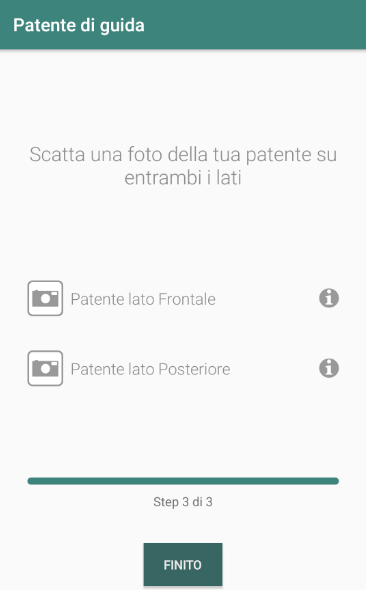
\includegraphics[width=0.5\textwidth]{res/images/patente3.png}\\
	\caption{Foto patente}
	\label{patente7}
\end{figure}
\pagebreak

Anche in questa sezione sono presenti degli aiuti all'utente per indicare quale lato inserire premendo sul tasto info.
\begin{figure}[H] 
	\centering 
	\includegraphics[width=0.5\textwidth]{res/images/patente3_1.png}\\
	\caption{Lato frontale}
	\label{patente8}
\end{figure}
Errore annesso:
\begin{figure}[H] 
	\centering 
	\includegraphics[width=0.5\textwidth]{res/images/patente3errore_front.png}\\
	\caption{Errore foto frontale}
	\label{patenteerror3}
\end{figure}
\pagebreak

\begin{figure}[H] 
	\centering 
	\includegraphics[width=0.5\textwidth]{res/images/patente3_2.png}\\
	\caption{Lato posteriore}
	\label{patente9}
\end{figure}
Errore annesso:
\begin{figure}[H] 
	\centering 
	\includegraphics[width=0.5\textwidth]{res/images/patente3errore.png}\\
	\caption{Errore foto posteriore}
	\label{patenteerror4}
\end{figure}
\pagebreak

	\item \textbf{Nome e cognome}: cliccando sull'icona a forma di penna a destra del nome si passa alla fase di inserimento e modifica;
	\begin{figure}[H] 
		\centering 
		\includegraphics[width=0.5\textwidth]{res/images/modifica_nome.png}\\
		\caption{Modifica del nome}
		\label{modificanome}
	\end{figure}
\pagebreak

		\item \textbf{Numero di cellulare}: cliccando sull'icona a forma di penna a destra del numero di cellulare si passa alla fase di inserimento e modifica;
	\begin{figure}[H] 
		\centering 
		\includegraphics[width=0.5\textwidth]{res/images/modifica_cellulare.png}\\
		\caption{Modifica del cellulare}
		\label{modificell}
	\end{figure}
\pagebreak

\item \textbf{Data di nascita}: cliccando sull'icona a forma di penna a destra della data di nascita si passa alla fase di inserimento e modifica;
\begin{figure}[H] 
	\centering 
	\includegraphics[width=0.5\textwidth]{res/images/modifica_data_nascita.png}\\
	\caption{Data di nascita}
	\label{modificanascita}
\end{figure}
\pagebreak

\item \textbf{Residenza}: cliccando sull'icona a forma di penna a destra della residenza si passa alla fase di inserimento e modifica;
\begin{figure}[H] 
	\centering 
	\includegraphics[width=0.5\textwidth]{res/images/modifica_residenza.png}\\
	\caption{Modifica della residenza}
	\label{modifiresidenza}
\end{figure}
\pagebreak
\end{itemize}

\subsection{Gioca}
